\chapter{Conice, cuadrice, forma canonică Jordan}

\section{* Forme biliniare}
\label{sec:biliniare}

\begin{definition}\label{def:forma-bil}
  Fie $V$ un spațiu vectorial și $F : V \times V \to \RR$ o aplicație.

  $F$ se numește \emph{formă biliniară} dacă satisface:
  \begin{enumerate}[(a)]
  \item $F(\alpha x + \beta y, z) = \alpha F(x, z) + \beta F(y, z)$;
  \item $F(x, \alpha y + \beta z) = \alpha F(x, y) + \beta F(x, z)$.
  \end{enumerate}
\end{definition}

\begin{definition}\label{def:bil-sim}
  O formă biliniară $F : V \times V \to \RR$ se numește \emph{simetrică} dacă
  $F(x, y) = F(y, x), \forall x, y \in V$.
\end{definition}


\begin{definition}\label{def:bil-neg-def}
  O formă biliniară simetrică $F$ se numește \emph{pozitiv (negativ) semidefinită}
  dacă $F(x, x) = 0$ (respectiv $F(x, x) \leq 0$), pentru orice $x \in V$.

  Dacă, în plus, $F(x, x) = 0$ numai pentru $x = 0_V$, ea se numește \emph{pozitiv % 
  (negativ) definită}.
\end{definition}

Exemple:
\begin{enumerate}[(1)]
\item Dacă $V$ este un spațiu euclidian real, atunci produsul scalar este o formă
  biliniară, simetrică și pozitiv definită.
\item Dacă $D \seq \RR^n$ este o submulțime deschisă, iar $f : D \to \RR$ este o
  funcție de clasă $C^2(D)$, atunci diferențiala a doua a lui $f$ este o formă
  biliniară și simetrică:
  \[
    F : \RR^n \times \RR^n \to \RR, F(h, k) = \sum_{i, j = 1}^n f_{x_i x_j}(h_i k_j),
  \]
  unde $(h_i), (k_j) \in \RR^n$.
\end{enumerate}

Folosind biliniaritatea, putem asocia unei forme pătratice o matrice într-o bază:
\[
  F(x, y) = F \Big( \sum_i x_i e_i \sum_j y_j e_j \Big) = %
  \sum_i \sum_j x_i y_j F(e_i, e_j).
\]

%%%%%%%%%%%%%%%%%%%%%%%%%%%%%%%%%%%%%%%%%%%%%%%%%%%%%%%%%%%%%%%%%%%%%%

\section{* Forme pătratice}
\label{sec:f-patr}

\begin{definition}\label{def:f-patr}
  Fie $F$ o formă biliniară și simetrică. Aplicația:
  \[
    Q : V \to \RR, Q(x) = F(x, x)
  \]
  se numește \emph{forma pătratică asociată formei biliniare simetrice $F$}.

  În acest context, $F$ se numește \emph{polara formei pătratice $Q$}.
\end{definition}

\begin{remark}\label{rk:patr-bil}
  Oricărei forme pătratice i se poate asocia o unică formă biliniară simetrică
  și reciproc.
\end{remark}

Asocierea formei pătratice rezultă din definiție, iar forma biliniară poate fi
definită astfel:
\begin{align*}
  Q(x + y) &= F(x + y, x + y) \\
           &= F(x, x) + 2F(x, y) + F(y, y) \\
           &= Q(x) + 2F(x, y) + Q(y) \\
  \Rightarrow F(x, y) &= \frac{1}{2} \big( Q(x, y) - Q(x) - Q(y) \big).
\end{align*}

De exemplu, produsul scalar, ca formă biliniară, induce pătratul normei, ca formă pătratică.

%%%%%%%%%%%%%%%%%%%%%%%%%%%%%%%%%%%%%%%%%%%%%%%%%%%%%%%%%%%%%%%%%%%%%%

\subsection{* Forma canonică}
\label{subsec:f-can}

Ne vor interesa problemele de aducere a unei forme pătratice la forma canonică:

\begin{definition}\label{def:f-can-patr}
  Spunem că forma pătratică $Q : V \to \RR$ este \emph{redusă la forma canonică}
  dacă găsim pentru $Q$ o scriere de forma:
  \[
    Q(x) = \sum_i b_i x_i^2,
  \]
  într-o anumită bază a lui $V$.
\end{definition}

\indent\indent Această metodă se bazează pe rezultatul următor:

\begin{theorem}[\textsc{C. F. Gauss}]
	Pentru orice formă pătratică $Q : V \to \mathbb{R}$, există o bază 
$\mathcal{B}$ a lui $V$ în care forma pătratică este redusă la forma canonică.
\end{theorem}

\begin{proof}
	Fie $B = \{e_1, \dots, e_n\}$ baza lui $V$ față de care forma pătratică $Q$
are scrierea: 
 \[
	Q(x) = \sum_{1 \leq i, j \leq n} a_{ij} x_i x_j.
\]

Vom distinge două cazuri:

(1) Dacă există cel puțin un indice $1 \leq i \leq n$ astfel încît 
$a_{ii} \neq 0$ (deoarece în expresia formei pătratice apare cel puțin un termen
la pătrat), atunci, printr-o eventuală renumerotare a indicilor (și, respectiv,
a vectorilor bazei $B$), putem presupune $a_{11} \neq 0$. În expresia formei
$Q$, regrupăm termenii:
\begin{align*}
Q(x) &= a_{11}x_1^2 + 2 \sum_{j = 2}^n a_{1j} x_1 x_j + 
                        \sum_{2 \leq i,j \leq n} a_{ij} x_i x_j \\
     &= \dfrac{1}{a_{11}} \big( a_{11} x_1 + a_{12} x_2 + \dots +
                  a_{1n} x_n \big)^2 - \dfrac{1}{a_{11}} \cdot
                  \sum_{2 \leq i, j \leq n} a_{1i} a_{1j} x_i x_j +
                  \sum_{2 \leq i, j \leq n} a_{ij} x_i x_j \\
     &= \dfrac{1}{a_{11}} \big( a_{11} x_1 + a_{12} x_2 + \dots +
                            + a_{1n} x_n \big)^2 +
                        \sum_{2 \leq i, j \leq n} a^{\prime}_{ij} x_i x_j,
\end{align*}
unde am notat $a^{\prime}_{ij} = a_{ij} \dfrac{a_{1i} a_{1j}}{a_{11}}$, pentru
orice indice $2 \leq i, j \leq n$.

Facem următoarele notații: 
 \[
	\begin{cases}	
	    x^{\prime}_1 &= a_{11}x_1 + a_{12} x_2 + \dots + a_{1n} x_n \\
	    x^{\prime}_2 &= x_2 \\
	    \dotfill \\
	    x^{\prime}_n = x_n.
    \end{cases}
\]

Cu aceasta, obținem: 
 \[
	Q(x) = \dfrac{1}{a_{11}} {x_1^{\prime}}^2 + 
	        \sum_{2 \leq i,j \leq n} a^{\prime}_{ij} x^{\prime}_i x^{\prime}_j.
\]

În această expresie, $x^{\prime}_1, x^{\prime}_2, \dots, x^{\prime}_n$ sînt
componentele vectorului $x$ în baza $B^{\prime} = \{e^{\prime}_i\}$. De remarcat
faptul că suma $\displaystyle\sum_{2 \leq i,j \leq n} a^{\prime}_{ij} 
x^{\prime}_i x^{\prime}_j$ care apare în expresia de mai sus este o formă 
pătratică cu $n - 1$ variabile. Așadar, după cel mult $n - 1$ astfel de pași,
obținem o bază $\overline{B} = \{\overline{e}_i \}$ a lui $V$, față de care
forma pătratică are forma canonică: 
 \[
	Q(x) = \alpha_1 \overline{x}_1^2 + \alpha_2 \overline{x}_2^2 + \dots
	            + \alpha_n \overline{x}_n^2.
\]

(2) Pentru al doilea caz, dacă toți coeficienții $a_{ii}$ sînt nuli, adică în 
forma pătratică apar doar termeni micști, presupunem, mai departe, că întreaga
formă nu este nulă, deci există $1 \leq i \neq j \leq n$, cu $a_{ij} \neq 0$.
Putem, din nou, să facem o eventuală renumerotare și să presupunem $a_{12} 
\neq 0$. Facem schimbările de coordonate: 
 \[
	\begin{cases}	
	    x_1 &= x^{\prime}_1 + x^{\prime}_2 \\
	    x_2 &= x^{\prime}_1 - x^{\prime}_2 \\
	    x_3 &= x^{\prime}_3 \\
	    \dotfill \\
	    x_n &= x^{\prime}_n. 
    \end{cases}
\]

Obținem: 
 \[
	Q(x) = 2a_{12} \Big[ (x^{\prime}_1)^2 - (x^{\prime}_2)^2 \Big] + \dots.
\]

În această expresie, avem cel puțin un termen la pătrat, deci putem continua
apoi procedeul pentru restul termenilor (cei omiși).
\end{proof}

Procedeul descris în această teoremă se numește \emph{metoda lui Gauss de a
reduce o formă pătratică la forma canonică}.

Să luăm un exemplu:

\begin{example}
	Fie forma pătratică $Q : \mathbb{R}^3 \to \mathbb{R}$, care, într-o bază
a spațiului $\mathbb{R}^3$ are expresia: 
 \[
	Q(x) = x_1^2 + 4x_2^2 + x_3^2 - 2x_1 x_2 + 2x_1 x_3.
\]

Folosim metoda lui Gauss. Deoarece în expresia acestei forme pătratice avem și
termeni la pătrat, ne situăm în primul caz din demonstrație. Urmăm procedeul
și avem:
\begin{align*}
Q(x) &= (x_1^2 - 2x_1 x_2 + 2x_1 x_3) + 4x_2^2 + x_3^2 \\
     &= (x_1 - x_2 + x_3)^2 - x_2^2 - x_3^2 + 2x_2 x_3 + 4x_2^2 + x_3^2 \\
     &= (x_1 - x_2 + x_3)^2 + 3x_2^2 + 2x_2 x_3 \\
     &= (x_1 - x_2 + x_3)^2 + \dfrac{1}{3} (9x_2^2 + 6x_2 x_3) \\
     &= (x_1 - x_2 + x_3)^2 + \dfrac{1}{3} (3x_2 + x_3)^2 - \dfrac{1}{3} x_3^2.
\end{align*}

Facem notațiile: 
 \[
	\begin{cases}	
	    \overline{x}_1 &= x_1 - x_2 + x_3 \\
	    \overline{x}_2 &= 3x_2 + x_3 \\
	    \overline{x}_3 &= x_3.
    \end{cases}
\]

Cu acestea, obținem forma canonică a formei pătratice: 
 \[
	Q(x) = \overline{x}_1^2 + \dfrac{1}{3} \overline{x}_2^2 - \dfrac{1}{3}
	        \overline{x}_3^2.
\]

Să determinăm și baza $\overline{B} = \{\overline{e}_1, \overline{e}_2,
\overline{e}_3\}$ în care s-a obținut această formă canonică. Pentru aceasta,
exprimăm componentele inițiale $\{x_1, x_2, x_3\}$ în funcție de componentele
$\{\overline{x}_1, \overline{x}_2, \overline{x}_3\}$ din baza $\overline{B}$: 
 \[
	\begin{cases}	
	    x_1 &= \overline{x}_1 + \dfrac{1}{3} \overline{x}_2 - \dfrac{4}{3}
	            \overline{x}_3 \\
	    x_2 &= \dfrac{1}{3} \overline{x}_2 - \dfrac{1}{3} \overline{x}_3 \\
	    x_3 &= \overline{x}_3.
    \end{cases}
\]

Rezultă că matricea de trecere de la baza inițială $B = \{e_1, e_2, e_3\}$ la
baza $\overline{B}$ este: 
 \[
	C = \begin{pmatrix}
	        1 & \frac{1}{3} & -\frac{4}{3} \\
	        0 & \frac{1}{3} & -\frac{1}{3} \\
	        0 & 0 & 1.
        \end{pmatrix}
\]

Așadar, vectorii bazei $\overline{B}$ sînt: 
 \[
	\begin{cases}	
	    \overline{e}_1 &= e_1 \\
	    \overline{e}_2 &= \dfrac{1}{3} e_1 + \dfrac{1}{3} e_2 \\
	    \overline{e}_3 &= -\dfrac{4}{3} e_1 - \dfrac{1}{3} e_2 + e_3.
    \end{cases}
\]
\end{example}

Să mai vedem un exemplu care să pună la lucru cazul al doilea din teoremă.

\begin{example}
	Fie forma pătratică: 
 \[
	Q : \mathbb{R}^3 \to \mathbb{R}, Q(x) = x_1 x_2 + x_2 x_3 + x_3 x_1.
\]

O vom aduce la forma canonică folosind metoda lui Gauss și vom specifica și
baza în care ea are această formă canonică.

Deoarece în expresia formei pătratice apar doar termeni micști, ne situăm în al
doilea caz din demonstrația teoremei. Facem schimbările de coordonate: 
 \[
	\begin{cases}	
	    x_1 &= x^{\prime}_1 + x^{\prime}_2 \\
	    x_2 &= x^{\prime}_1 - x^{\prime}_2 \\
	    x_3 &= x^{\prime}_3.
    \end{cases}
\]

Forma pătratică devine:
\begin{align*}
Q(x) &= (x^{\prime}_1)^2 - (x^{\prime}_2)^2 + (x^{\prime}_1 - x^{\prime}_2)
        \cdot x^{\prime}_3 + x^{\prime}_3(x^{\prime}_1 + x^{\prime}_2) \\
     &= (x^{\prime}_1)^2 - (x^{\prime}_2)^2 + 2x^{\prime}_1 x^{\prime}_3 \\
     &= \big[ (x^{\prime}_1)^2 + 2x^{\prime}_1 x^{\prime}_3 \big] -
        (x^{\prime}_2)^2 \\
     &= (x^{\prime}_1 + x^{\prime}_3)^2 - (x^{\prime}_2)^2 - (x^{\prime}_3)^2.
\end{align*}

Facem altă schimbare de coordonate: 
 \[
	\begin{cases}	
	    \overline{x}_1 &= x^{\prime}_1 + x^{\prime}_3 \\
	    \overline{x}_2 &= x^{\prime}_2 \\
	    \overline{x}_3 &= x^{\prime}_3.
    \end{cases}
\]

Cu acestea, rezultă forma canonică: 
 \[
	Q(x) = \overline{x}_1^2 - \overline{x}_2^2 - \overline{x}_3^2.
\]

De asemenea, din schimbările de variabile rezultă și schimbările de coordonate: 
 \[
	\begin{cases}	
	    \overline{x}_1 &= \dfrac{1}{2} x_1 + \dfrac{1}{2} x_2 + x_3 \\
	    \overline{x}_2 &= \dfrac{1}{2} x_1 - \dfrac{1}{2} x_2 \\
	    \overline{x}_3 &= x_3.
    \end{cases}
\]
\end{example}

%%%%%%%%%%%%%%%%%%%%%%%%%%%%%%%%%%%%%%%%%%%%%%%%%%%%%%%%%%%%%%%%%%%%%%%%%%%%%%%%

\subsection{* Metoda lui Jacobi}

\indent\indent Cea de-a doua metodă pe care o studiem este \emph{metoda lui
Jacobi}, care se bazează pe următorul rezultat:
\begin{theorem}[\textsc{C. Jacobi}]
	Fie $V$ un spațiu vectorial și $B = \{e_1, \dots e_n\}$ o bază a lui $V$.
Fie $Q : V \to \mathbb{R}$ o formă pătratică, cu expresia în baza $B$: 
 \[
	Q(x) = \sum_{1 \leq i, j \leq n} a_{ij} x_i x_j.
\]

Dacă matricea $A = (a_{ij})$ asociată formei pătratice $Q$ în baza $B$ are toți
minorii principali: 
 \[
	\Delta_1 = a_{11}, \quad \Delta_2 = \begin{vmatrix}
	                                        a_{11} & a_{12} \\
	                                        a_{12} & a_{22}
                                        \end{vmatrix}, \quad
    \Delta_3 = \begin{vmatrix}
	               a_{11} & a_{12} & a_{13} \\
	               a_{21} & a_{22} & a_{23} \\
	               a_{31} & a_{32} & a_{33}
               \end{vmatrix}, \dots, \Delta_n = \det(A)
\]
nenuli, atunci există o bază $\overline{B}$ a lui $V$ față de care $Q$ are
forma canonică: 
 \[
	Q(x) = \dfrac{1}{\Delta_1} \overline{x}_1^2 + \dfrac{\Delta_1}{\Delta_2}
	        \overline{x}_2^2 + \dfrac{\Delta_2}{\Delta_3} \overline{x}_3^2 +
	        \dots + \dfrac{\Delta_{n-1}}{\Delta_n} \overline{x}_n^2.
\]
\end{theorem}

\begin{proof}
	Fie $F : V \times V \to \mathbb{R}$ polara formei pătratice $Q$. Căutăm
vectorii bazei $\overline{B}$, de forma:
\begin{equation}
    \label{equation:sistem-coef-jacobi}
	\begin{cases}	
	    \overline{e}_1 &= c_{11} e_1 \\
	    \overline{e}_2 &= c_{12} e_1 + c_{22}e_2 \\
	    & \dotfill \\
	    \overline{e}_i &= c_{1i}e_1 + c_{2i} e_2 + \dots + c_{ii}e_i \\
	    & \dotfill \\
	    \overline{e}_n &= c_{1n}e_1 + c_{2n} e_2 + \dots + c_{nn} e_n.
    \end{cases}
\end{equation}

Coeficienții $c_{ij}$ se determină din condițiile:
\begin{align*}
	F(\overline{e}_i, e_j) &= 0, \forall 1 \leq j < i \leq n \\
	F(\overline{e}_i, e_i) &= 1, \forall 1 \leq i \leq n.
\end{align*}
Condițiile se obțin din faptul că matricea asociată formei pătratice $Q$ în
baza $\overline{B}$ să fie diagonală, cu $c_{ii}$ pe diagonală.

Fie $i \in \{1, 2, \dots, n\}$ arbitrar fixat. Avem: 
 \[
	F(\overline{e}_i, e_j) = F \Big( \sum_{k = 1}^i c_{ki} e_k e_j \Big) =
	                         \sum_{k = 1}^i c_{ki} F(e_k, e_j) =
	                         \sum_{k = 1}^i c_{ki} a_{kj},
\]
de unde, ținînd cont că $a_{kj} = a_{jk}$, obținem sistemul: 
 \[
	\begin{cases}	
	    a_{11} c_{1i} + a_{12} c_{2i} + \dots + a_{1i} c_{ii} &= 0 \\
	    a_{12} c_{1i} + a_{22} c-{2i} + \dots + a_{2i} c_{ii} &= 0 \\
	    \dotfill \\
	    a-{1, i-1} c_{1i} + a_{2, i-1}c_{2i} + \dots + a_{i-1, i} c_{ii} &= 0 \\
	    a_{1i} c_{1i} + a_{2i} c_{2i} + \dots + a_{ii} c_{ii} &= 1.
    \end{cases}
\]

Remarcăm că determinantul matricei acestui sistem este minorul principal
$\Delta_i$, care, conform ipotezei, este nenul. Așadar, putem rezolva sistemul
cu regula lui Cramer: 
 \[
	c_{ii} = \dfrac{1}{\Delta_i} \cdot \Delta_{i-1}.
\]

Mai folosim faptul că: 
 \[
	\det \begin{pmatrix}
	          c_{11} & c_{12} & \dots & c_{1n} \\
	          0 & c_{12} & \dots & c_{2n} \\
	          \dots & \dots & \dots & \dots \\
	          0 & 0 & \dots & c_{nn}
         \end{pmatrix} = c_{11} c_{22} \cdots c_{nn} = \dfrac{1}{\Delta_n} 
    \neq 0
\]
și, în plus, că $B = \{e_e, e_2, \dots, e_n\}$ este o bază a lui $V$, rezultă și
că $\overline{B} = \{\overline{e}_1, \overline{e}_2, \dots, \overline{e}_n \}$
este o bază a lui $V$. Deoarece: 
 \[
	F(\overline{e}_i. \overline{e}_j) = \begin{cases}	
	                                        0, & i \neq j \\
	                                        c_{ii}, & i = j,
                                         \end{cases}
\]
rezultă concluzia teoremei.
\end{proof}

Să mai facem o observație importantă. Spre deosebire de metoda lui Gauss, care
poate fi aplicată oricărei forme pătratice, metoda lui Jacobi cere în mod 
necesar ca toți minorii principali ai matricei atașate formei pătratice în baza
inițială să fie nenuli. Altfel, această metodă nu se poate aplica.

Să o vedem într-un exemplu:
\begin{example}
	Reducem la forma canonică forma pătratică: 
 \[
	Q : \mathbb{R}^3 \to \mathbb{R}, 
	Q(x) = 3x_1^2 + 3x_2^2 + 2x_1 x_2 + 4x_1x_3 + 4x_2x_3.
\]

Matricea asociată formei pătratice $Q$ în baza canonică a lui $\mathbb{R}^3$
este: 
 \[
	A = \begin{pmatrix}
	        3 & -1 & 2 \\
	        -1 & 3 & 2 \\
	        2 & 2 & 0
        \end{pmatrix}
\]

Minorii principali ai matricei sînt toți nenuli, după cum se poate verifica
simplu. Așadar, putem aplica metoda lui Jacobi și forma canonică a formei 
pătratice $Q$ este, direct:
\begin{align*}
	Q(x) &= \dfrac{1}{\Delta_1} \overline{x}_1^2 + \dfrac{\Delta_1}{\Delta_2}
	        \overline{x}_2^2 + \dfrac{\Delta_2}{\Delta_3} \overline{x}_3^2 \\
	     &= \dfrac{1}{3} \overline{x}_1^2 + \dfrac{3}{8} \overline{x}_2^2 -
	        \dfrac{1}{4} \overline{x}_3^2.
\end{align*}

Pentru a obține baza în care avem această formă, se rezolvă sistemul
~\eqref{equation:sistem-coef-jacobi}.
\end{example}

%%%%%%%%%%%%%%%%%%%%%%%%%%%%%%%%%%%%%%%%%%%%%%%%%%%%%%%%%%%%%%%%%%%%%%%%%%%%%%%%

\subsection{* Metoda transformărilor ortogonale}

\indent\indent În fine, ultima metodă algoritmică pe care o discutăm este
\emph{metoda transformărilor ortogonale}. Ea se bazează pe următorul rezultat, 
care, la rîndul lui, pune în prim-plan bazele ortonormate din spații vectoriale:
\begin{theorem}
	Fie $V$ un spațiu euclidian de dimensiune $n$ și $Q$ o formă pătratică.

Există o bază ortonormată a lui $V$ în raport cu care forma pătratică $Q$ este
redusă la forma canonică.
\end{theorem}

\begin{proof}
	Știm că există o bază ortonormată pentru $V$. Fie aceasta $\mathcal{B} = \{
e_1, e_2, \dots, e_n\}$. Fie $A = (a_{ij})$ matricea asociată formei pătratice
$Q$ în baza $\mathcal{B}$. Deoarece $A$ este matrice simetrică, rezultă că
există două matrice ortogonale $C = (c_{ij})$ și $D$ -- o matrice diagonală
cu $\lambda_1, \lambda_2, \dots, \lambda_n$, care reprezintă forma diagonală a
matricei $A$, astfel încît: 
 \[
	A = CDC^T.
\]

Construim acum baza $\overline{\mathcal{B}} = \{\overline{e}_1, \overline{e_2},
\dots, \overline{e}_n\}$ a lui $V$, astfel încît matricea de trecere de la 
$\mathcal{B}$ la $\overline{\mathcal{B}}$ să fie chiar $C$, adică: 
 \[
	\begin{cases}	
	    \overline{e}_1 = c_{11} e_1 + c_{21}e_2 + \dots + c_{n1} e_n \\
	    \overline{e}_2 = c_{12} e_1 + c_{22} e_2 + \dots + c_{n2} e_n \\
	    \dotfill \\
	    \overline{e}_n = c_{1n} e_1 + c_{2n} e_2 + \dots + c_{nn} e_n
    \end{cases}
\]

Ținem cont de faptul că $\overline{B} = \{e_1, \dots, e_n\}$ este o bază
ortonormată, iar $C$ este o matrice ortogonală. Deci obținem relațiile:
\begin{align*}
	\langle \overline{e}_i, \overline{e}_i \rangle &=
	\Big\langle \sum_{k = 1}^n c_{ki} e_k, \sum_{j = 1}^n c_{ji} e_j 
	\Big \rangle \\
	&= \sum_{1 \leq k, j \leq n} c_{ki} c_{ji} \langle e_k, e_j \rangle \\
	&= \sum_{k=1}^n c_{ki}^2 = 1, \forall 1 \leq i \leq n \\
    \langle \overline{e}_i, \overline{e}_j \rangle &=
    \Big\langle \sum_{k=1}^n c_{ki} e_k, \sum_{p=1}^n c_{pj}e_p 
    \Big \rangle \\
    &= \sum_{1 \leq k,p \leq n} c_{ki} c_{pj} \langle e_k, e_p \rangle \\
    &= \sum_{k = 1}^n c_{ki} c_{kj} \\
    &= 0, \forall i \neq j.
\end{align*}

Rezultă $\overline{\mathcal{B}} = \{\overline{e}_1, \dots, \overline{e}_n \}$
este o bază ortonormată a lui $V$.

Fie $F$ polara formei pătratice $Q$. Rezultă că matricea asociată lui $F$ în
baza $\overline{\mathcal{B}}$ este diagonală, cu $\lambda_i$ pe diagonală și
deci, forma pătratică $Q$ va avea scrierea în baza $\overline{\mathcal{B}}$: 
 \[
	Q(x) = \lambda_1 \overline{x}_1^2 + \lambda_2 \overline{x}_2^2 + \dots
	        + \lambda_n \overline{x}_n^2,
\]
adică este redusă la forma canonică, ceea ce se dorea.
\end{proof}

Trebuie remarcat faptul că, încă din enunț, este clar că metoda aceasta se 
aplică doar spațiilor euclidiene. Dar, cum spațiul $\mathbb{R}^n$ este 
euclidian, vom avea suficiente exemple și exerciții în care să o punem la lucru.

Sumarizînd, algoritmul de aplicat, așa cum reiese din demonstrația anterioară,
cuprinde:
\begin{enumerate}[(1)]
	\item Scriem matricea $A$ atașată formei pătratice;
	\item Găsim, prin rezolvarea ecuației caracteristice,
$\det(A - \lambda I_n) = 0$, valorile proprii $\lambda_i$, cu $1 \leq i \leq p$,
care au ordinele de multiplicitate $n_i$ și determinăm subspațiile vectorilor
proprii $V(\lambda_i)$, care corespund acestor valori proprii.
    \item Pentru fiecare subspațiu $V(\lambda_i)$, determinăm cîte o bază
ortonormată $\mathcal{B}_i$;
    \item Forma canonică a formei pătratice este, cu acestea: 
 \[
	Q(x) = \lambda_1 \overline{x}_1^2 + \lambda_2 \overline{x}_2^2 + \dots
	         + \lambda_n \overline{x}_n^2,
\]
cu observația că fiecare valoare proprie apare de un număr de ori egal cu
multiplicitatea sa. Baza ortonormată în care se obține această formă canonică
este dată de reuniunea $\overline{\mathcal{B}} = \mathcal{B}_1 \cup 
\mathcal{B}_2 \cup \dots \cup \mathcal{B}_n$.
\end{enumerate}

Aplicăm această metodă pe un exemplu.

\begin{example}
	Fie forma pătratică: 
 \[
	Q : \mathbb{R}^3 \to \mathbb{R}, 
	Q(x) = 3x_1^2 + 3x_2^2 - 2x_1 x_2 + 4x_1 x_3 + 4x_2 x_3.
\]

O vom aduce la forma canonică folosind metoda transformărilor ortogonale și,
totodată, vom determina și baza ortonormată în care $Q$ are acea formă.

Matricea asociată formei pătratice $Q$ în baza canonică este: 
 \[
	A = \begin{pmatrix}
	        3 & -1 & 2 \\
	        -1 & 3 & 2 \\
	        2 & 2 & 0
        \end{pmatrix}.
\]

Determinăm valorile proprii, prin rezolvarea ecuației caracteristice. Rezultă: 
 \[
	\lambda_1 = -2, \quad \lambda_2 = \lambda_3 = 4.
\]

Vectorii proprii corespunzători valorii proprii $\lambda_1 = -2$ generează
subspațiul invariant: 
 \[
	V(-2) = \{(-\alpha, -\alpha, 2 \alpha)^T \mid \alpha \in \mathbb{R} \}.
\]

O bază pentru acest subspațiu este, de exemplu, $\{(-1, -1, 2)^T\}$. Aplicăm
algoritmul Gram-Schmidt pentru ortonormare și obținem: 
 \[
	\mathcal{B}_1 = \Big\{ \Big( -\dfrac{1}{\sqrt{6}}, - \dfrac{1}{\sqrt{6}},
	\dfrac{2}{\sqrt{6}} \Big)^T \Big\}.
\]

Procedăm similar pentru valoarea proprie $\lambda = 4$ și obținem: 
 \[
	V(4) = \{(-\alpha + 2 \beta, \alpha, \beta)^T \mid \alpha, \beta 
	\in \mathbb{R} \}.
\]

Alegem $e_2 = (-1, 1, 0)^T \in V(4)$ și vrem să determinăm $e_3 \perp e_2$, cu
$e_3 = (- \alpha_3 + 2 \beta_3, \alpha_3, \beta_3)^T$. Condiția de 
perpendicularitate înseamnă $\langle e_2, e_3 \rangle = 0$, deci obținem:
$\beta_3 = \alpha_3 \Longrightarrow e_3 = (\alpha_3, \alpha_3, \alpha_3)^T$.
Ortonormăm această bază și obținem: 
 \[
	\mathcal{B}_2 = \Big\{ \Big( -\dfrac{1}{\sqrt{2}}, \dfrac{1}{\sqrt{2}}, 0
	 \Big)^T, \Big( \dfrac{1}{\sqrt{3}}, \dfrac{1}{\sqrt{3}}, 
	 \dfrac{1}{\sqrt{3}} \Big)^T \Big\}.
\]

Forma canonică a formei pătratice date este, atunci: 
 \[
	Q(x) = -2 \overline{x}_1^2 + 4\overline{x}_2^2 - 4 \overline{x}_3^2.
\]

Această formă se obține în baza ortonormată 
$\overline{\mathcal{B}} = \mathcal{B}_1 \cup \mathcal{B}_2$.
\end{example}

\begin{remark}
	De remarcat faptul că, pornind cu aceeași formă pătratică și aplicînd metode
diferite de aducere la forma canonică, putem obține rezultate diferite.

În secțiunea următoare, vom identifica un invariant al formei canonice.
\end{remark}

%%%%%%%%%%%%%%%%%%%%%%%%%%%%%%%%%%%%%%%%%%%%%%%%%%%%%%%%%%%%%%%%%%%%%%%%%%%%%%%%

\section{* Signatura unei forme pătratice. Teorema inerției}

\begin{definition}
	Fie $Q$ o formă pătratică, ce are forma canonică: 
 \[
	Q(x) = \sum_{i = 1}^n a_i \overline{x}_i^2.
\]

Presupunem că în această scriere sînt $p$ coeficienți strict pozitivi, $q$
coeficienți strict negativi, iar $r = n - (p + q)$ coeficienți sînt nuli.

Tripletul $(p, q, r)$ se numește \emph{signatura formei pătratice}.
\end{definition}

Acesta este invariantul din forma canonică a unei forme pătratice, după cum
arată teorema următoare:

\begin{theorem}[Teorema inerției]
	Signatura unei forme pătratice este un invariant al formei canonice, adică
este aceeași în orice formă canonică a formei pătratice respective.
\end{theorem}

\begin{proof}
	Fie $Q : V \to \mathbb{R}$ o formă pătratică și $B_1 = \{e_1, \dots, e_n\}$,
$B_2 = \{f_1, \dots, f_n\}$ două baze ale lui $V$, în raport cu care $Q$ are
formele canonice: 
 \[
	Q(x) = \sum_{i=1}^n b_i \overline{x}_i^2, \quad 
	Q(x) = \sum_{i=1}^n b_i \widetilde{x}_i^2.
\]

Presupunem că signatura în prima scriere este $(p_1, q_1, r_1)$, iar în a doua,
$(p_2, q_2, r_2)$. Printr-o eventuală rearanjare a termenilor, putem presupune
că primii $p_1$ (respectiv $p_2$) coeficienți sînt strict pozitivi, apoi
următorii $q_1$ (respectiv $q_2$) sînt negativi, iar ultimii $r_1$, respectiv
$r_2$ sînt nuli.

Să presupunem că $p_1 > p_2$. Fie $V_1 = \dr{Sp} \{e_1, \dots e_{p_1}\}$ și
$V_2 = \dr{Sp} \{e_{p_2 + 1}, \dots, e_n\}$. Rezultă: 
 \[
	\dim_{\mathbb{R}} V_1 + \dim_{\mathbb{R}} V_2 = p_1 + n - p_2 > n.
\]

Așadar, există o intersecție nevidă între cele două și avem, conform teoremei
dimensiunii (Grassmann): 
 \[
	n \geq \dim_{\mathbb{R}}(V_1 + V_2) = \dim_{\mathbb{R}} V_1 + 
	\dim_{\mathbb{R}} V_2 - \dim_{\mathbb{R}} (V_1 \cap V_2) > 
	n - \dim_{\mathbb{R}} (V_1 \cap V_2).
\]

Deci $V_1 \cap V_2 \neq \{0_V\}$ și putem considera un vector nenul $x^\ast$ în
$V_1 \cap V_2$.

Pe de o parte, deoarece $x^\ast \in V_1$, avem că el se poate scrie în baza
corespunzătoare, $x^\ast = \overline{x}_1 e_1 + \dots + \overline{x}_p e_p$,
de unde deducem: 
 \[
	Q(x^\ast) = \sum_{i=1}^p a_i \overline{x}_i^2 \geq 0.
\]

Pe de altă parte, deoarece $x^\ast \in V_2$, avem și scrierea sa în baza
$B_2$, $x^\ast = \widetilde{x}_{p_2 + 1} f_{p_2 + 1} + \dots + 
                 \widetilde{x}_n f_n$. Deci: 
 \[
	Q(x^\ast) = \sum_{i = p_2 + 1}^n b_i \widetilde{x}_i^2 \leq 0.
\]

Din relațiile de mai sus, rezultă că $Q(x^\ast) = 0$, ceea ce implică faptul
că el are toate coordonatele nule, deci $x^\ast = 0_V$, contradicție.

Așadar, presupunerea $p_1 > p_2$ este falsă și similar se arată că nu putem avea
nici inegalitatea inversă și la fel pentru $q_1 = q_2$.
\end{proof}

\begin{definition}
	Spunem că o formă pătratică $Q : V \to \mathbb{R}$ este \emph{pozitiv 
(negativ) definită} dacă $Q(x) > 0$ (respectiv $Q(x) < 0$), pentru orice
$x \in V - \{0_V\}$. 

Evident, această definiție este echivalentă cu faptul că polara ei, $F$,
este pozitiv (respectiv negativ) definită.
\end{definition}

Următorul rezultat ne ajută să decidem cînd este o formă pătratică pozitiv
definită.

\begin{theorem}[Criteriul lui \textsc{Sylvester}]
	Fie $Q : V \to \mathbb{R}$ o formă pătratică și $B = \{e_1, \dots, e_n\}$
o bază a lui $V$, iar $A = (a_{ij})$ matricea asociată formei pătratice
$Q$ în baza $B$. Fie $\Delta_1, \dots, \Delta_n$ minorii principali ai matricei
$A$. Atunci:
\begin{enumerate}[(a)]
	\item $Q$ este pozitiv definită dacă și numai dacă $\Delta_i > 0$, pentru
toți $1 \leq i \leq n$;
    \item $Q$ este negativ definită dacă și numai dacă $(-1)^i \Delta_i > 0$,
pentru orice $1 \leq i \leq n$.
\end{enumerate}
\end{theorem}

De asemenea, o consecință imediată, așteptată, este următoarea:

\begin{proposition}
	Forma pătratică este pozitiv definită dacă și numai dacă matricea ei 
asociată este pozitiv definită.	
\end{proposition}

Știm, de asemenea, că între mulțimea formelor pătratice $Q : V \to \mathbb{R}$ 
și mulțimea matricelor simetrice există o corespondență bijectivă. Astfel că,
folosind și propoziția anterioară, putem reformula criteriul lui Sylvester
astfel:

\begin{theorem}
	O matrice simetrică este pozitiv definită dacă are toți minorii principali 
strict pozitivi.
\end{theorem}

%%%%%%%%%%%%%%%%%%%%%%%%%%%%%%%%%%%%%%%%%%%%%%%%%%%%%%%%%%%%%%%%%%%%%%

\section{Conice}

\indent\indent Studiul conicelor, ca obiecte geometrice, are o vechime 
considerabilă, fiind discutate încă din vremea lui Euclid și Grecia Antică.
Appollonius din Perga (262 -- 190 î. Hr.) a fost cel care le-a dat pentru prima
dată numele pe care le folosim și astăzi, anume elipsă, parabolă și hiperbolă.

În perioada Renașterii și ulterior, conicele au devenit din ce în ce mai
importante și studiate, prin prisma relevanței lor în fizică. Mișcările 
planetare și alte traiectorii studiate de Kepler, Galilei și alții, dar și în
scopuri geometrice pure la Descartes, Fermat, Desargues, Pascal și alții au
constituit cadrul în care teoria conicelor a evoluat.

Contextul geometric inițial a fost acela al secțiunilor determinate de un con
infinit, intersectat cu un plan, în diverse configurații. De asemenea, pe lîngă
această definiție geometrică simplă și generală, ele se pot studia și cu 
ajutorul formelor pătratice din spații vectoriale -- abordare pe care o vom lua
în cele ce urmează.

Considerăm, așadar, un plan $E_2$, cu un reper cartezian $\{0,\vec{i},\vec{j}\}$
prin care planul se poate identifica cu $\mathbb{R}^2$. Acest model ne va 
permite să descriem figurile cu ajutorul ecuațiilor și inecuațiilor asociate
unor funcții reale.

Fie o formă pătratică afină $g : \mathbb{R}^2 \to \mathbb{R}$, definită prin: 
 \[
	g(x,y) = a_{11} x^2 + 2a_{12}xy + a_{22}y^2 + 2a_{10}x + 2a_{20}y + a_{00},
\]
cu $a_{11}^2 + a_{12}^2 + a_{22}^2 \neq 0$.

Atunci:

\begin{definition}

	Mulțimea de nivel constant zero: 
 \[
    \Gamma = \{M(x,y) \mid (x,y) \in \mathbb{R}^2, g(x,y) = 0 \}
\]
se numește \emph{conică} sau \emph{curbă algebrică de ordinul al doilea}.

Notăm aceasta cu $\Gamma: g(x,y) = 0$.
\end{definition}

Să remarcăm că, din punct de vedere topologic, conicele sînt mulțimi închise
în $\mathbb{R}^2$, deoarece $\{0\}$ este mulțime închisă în $\mathbb{R}$, iar
$\Gamma$, care este imaginea sa inversă prin funcția continuă $g$ este, de
asemenea, închisă.

Problema principală căreia se adresează în primă fază studiul conicelor este 
aceea de a arăta că orice conică este congruentă cu una din mulțimile cunoscute:
cerc, elipsă, hiperbolă, parabolă, pereche de drepte, punct sau mulțime vidă.

Pentru aceasta, vom folosi o serie de transformări geometrice, precum rotația
și translația, față de care conica de interes să aibă o formă canonică.

În calcule, vor interveni următoarele numere asociate polinoamelor $g(x, y)$ ca
mai sus:
\begin{align*}
	\Delta &= \begin{vmatrix}
	              a_{11} & a_{12} & a_{10} \\
	              a_{12} & a_{22} & a_{20} \\
	              a_{10} & a_{20} & a_{00}
              \end{vmatrix} \\
    \delta &= \begin{vmatrix}
	              a_{11} & a_{12} \\
	              a_{21} & a_{22}
              \end{vmatrix} \\
    I &= a_{11} + a_{22} \\
    K &= \delta + \begin{vmatrix}
	                  a_{11} & a_{10} \\
	                  a_{10} & a_{00}
                  \end{vmatrix} + \begin{vmatrix}
	                                  a_{22} & a_{20} \\
	                                  a_{20} & a_{00}
                                  \end{vmatrix}
\end{align*}

\begin{remark}
	Atunci cînd se fac rotații și translații asupra unei conice, se poate arăta
că numerele de mai sus sînt invariante, motiv pentru care se vor numi 
\emph{invarianți metrici} ai conicei (rotația și translația fiind izometrii).

Ultimul număr asociat, $K$, este invariat doar de rotații și, de aceea, se mai
numește \emph{semi-invariant} metric al conicei.
\end{remark}

Pe scurt, clasificarea conicelor este dată în tabelul următor:

\begin{center}
\begin{tabular}{| c | c | c | c | c | c |}
    \hline
   $\delta$ & $\Delta$ & $I \Delta$ & $K$ & \textbf{Conica} & \textbf{Genul} \\
   \hline \hline
           & $\neq 0$ & $<0$ & & Elipsă &        \\
    $ > 0$ & $\neq 0$ & $>0$ & & Conica vidă & \textbf{Gen eliptic} \\
           & $= 0$    &      & & Punct (dublu) &  \\
    \hline \hline 
           & $ \neq 0 $ & & & Hiperbolă &  \\
    $ < 0$ & $ \neq 0 $ & & & Hiperbolă & \textbf{Gen hiperbolic} \\
           & $ = 0$     & & & Pereche de drepte concurente & 
                                          \\
    \hline \hline
           & $\neq 0$ &  &  & Parabolă &  \\
    $ = 0$ & $= 0$ & & < 0 & Pereche de drepte paralele &
                                        \textbf{Gen parabolic} \\
           & $= 0$ & & $=0$ & Pereche de drepte confundate & 
                                         \\
           & $= 0$ &  & $ > 0$ & Conica vidă & \\
    \hline
\end{tabular}
\end{center}

După cum se vede din tabel, invariantul $\delta$ ne dă \emph{genul conicei},
în timp ce invariantul $\Delta$ ne dă degenerarea.

În cazul hiperbolic, dacă se anulează invariantul $I$, sîntem conduși la o
hiperbolă echilateră, în care asimptotele sînt perpendiculare, iar în cazul
degenerat, cu $\Delta = 0$, hiperbola este redusă la o pereche de drepte
perpendiculare.

Cazurile principale, prezentate în tabel, împreună cu ecuațiile lor, sînt
redate în figura \ref{figure:conice}.

\begin{figure}[!h]
    \centering
    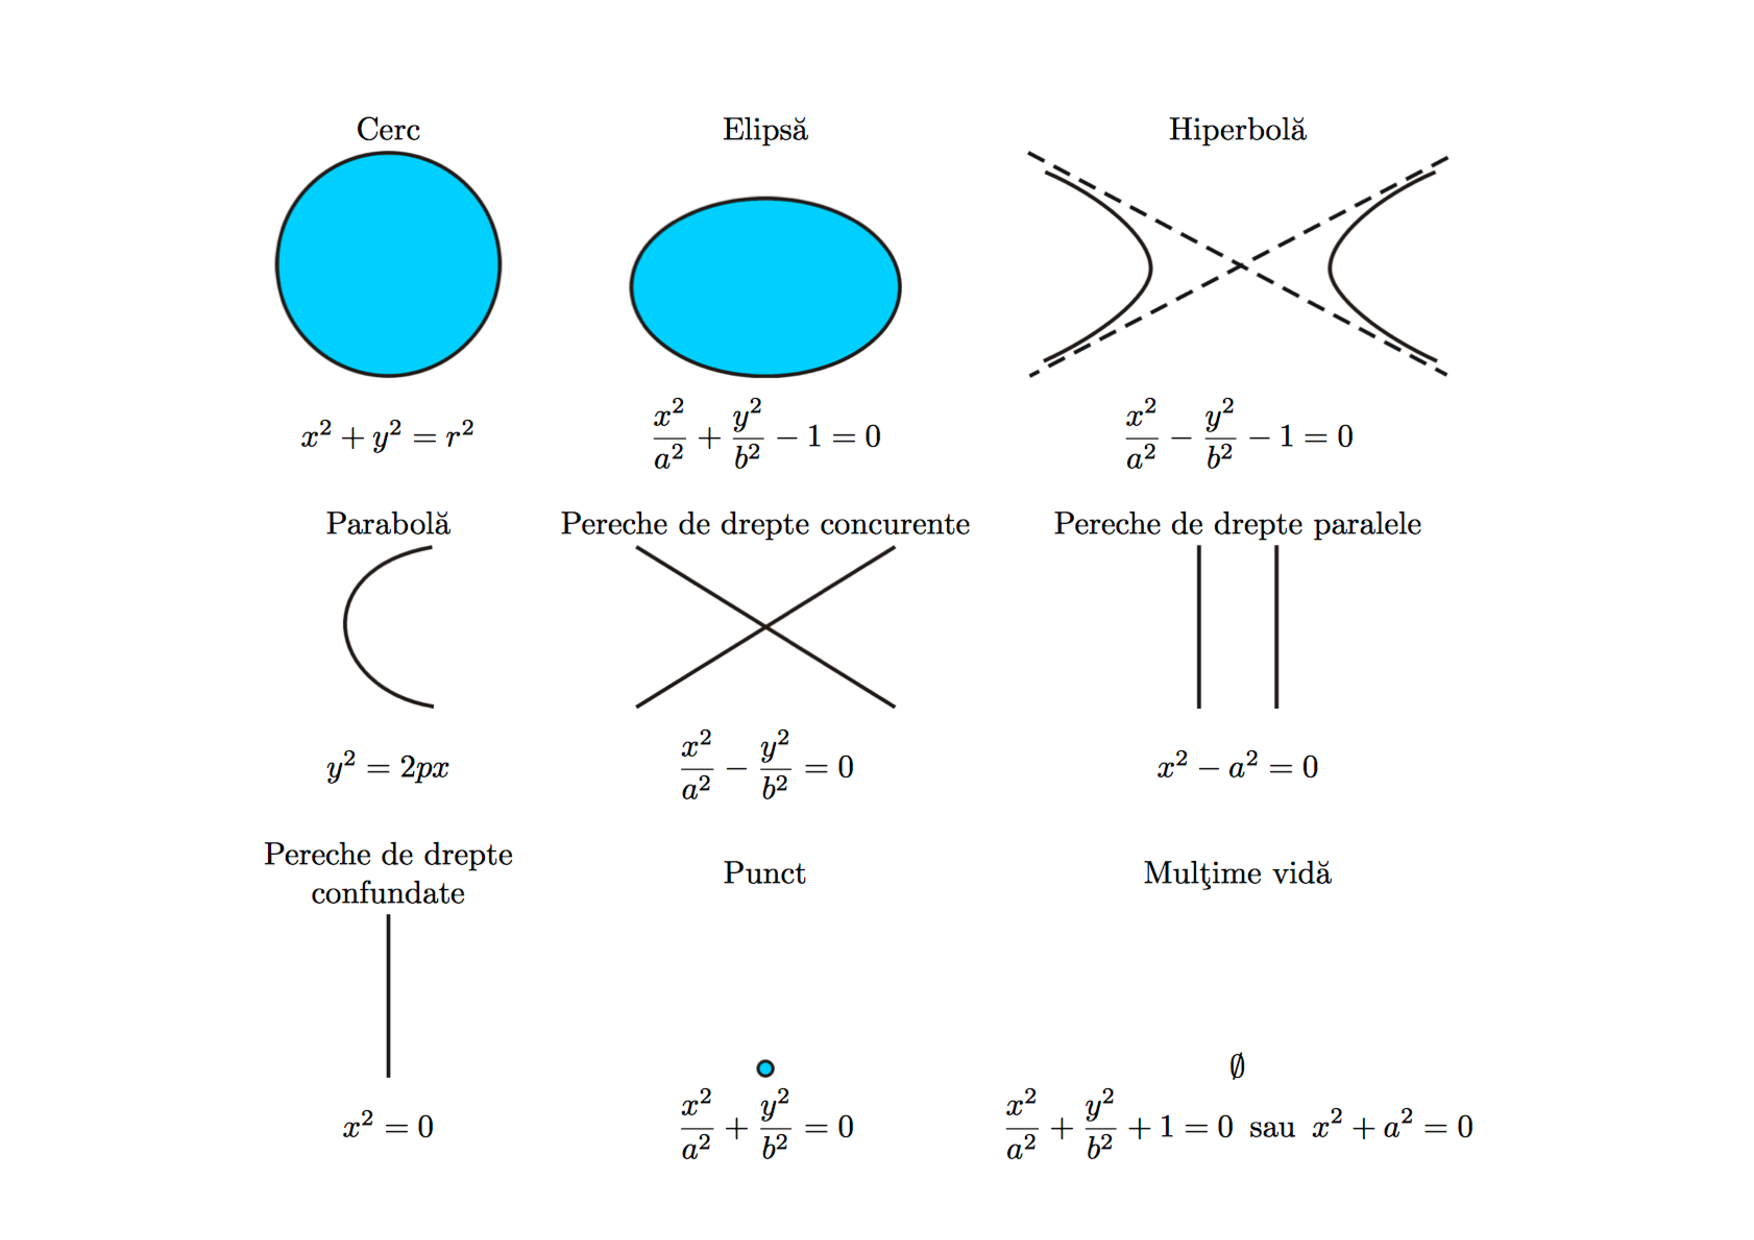
\includegraphics[scale = 0.6]{figs/conice}
    \caption{Conice și ecuațiile lor}
    \label{figure:conice}
\end{figure}

Punctele critice ale funcției $g$ se determină folosind instrumentele cunoscute
de analiză multidimensională. Astfel, avem de rezolvat sistemul liniar: 
 \[
	\begin{cases}	
	    \dfrac{1}{2} \dfrac{\partial g}{\partial x} &=
	    a_{11} x + a_{12} y + a_{10} = 0 \\
	    \dfrac{1}{2} \dfrac{\partial g}{\partial y} &= 
	    a_{12} x + a_{22} y + a_{20} = 0.
    \end{cases}
\]

Determinantul acestui sistem liniar este chiar: 
 \[
	\delta = \begin{vmatrix}
	             a_{11} & a_{12} \\
	             a_{12} & a_{22}
             \end{vmatrix}.
\]

Rezultă, din teoria sistemelor liniare, că, dacă $\delta \neq 0$, atunci 
sistemul are soluție unică, deci funcția are un singur punct critic.

Din configurația geometrică, interpretată algebric, rezultă:

\begin{theorem}
	Punctul $M_0(x_0, y_0)$ este centru de simetrie al conicei 
$\Gamma : g(x, y) = 0$ dacă și numai dacă $M_0(x_0, y_0)$ este un punct critic
al funcției $g$.
\end{theorem}

\begin{proof}
	Facem translația $x = x_0 + x^{\prime}$ și $y = y_0 + y^{\prime}$. Atunci
ecuația conicei devine: 
 \[
	a_{11} {x^{\prime}}^2 + 2a_{12}x^{\prime}y^{\prime} + a_{22} {y^{\prime}}^2
	+ x^{\prime}g_{x_0} + y^{\prime} g_{y_0} + g(x_0, y_0) = 0,
\]
unde $g_{x_0} = \dfrac{\partial g}{\partial x}(x_0, y_0)$, iar
$g_{y_0} = \dfrac{\partial g}{\partial y}(x_0, y_0)$.

Originea $M_0(x_0, y_0)$ a reperului translatat este centru de simetrie dacă
și numai dacă odată cu un punct arbitrar $(x^{\prime}, y^{\prime})$, conica
$\Gamma$ conține și punctul $(-x^{\prime}, -y^{\prime})$, adică are loc: 
 \[
	a_{11} {x^{\prime}}^2 + 2a_{12} x^{\prime} y^{\prime} + a_{22}{y^{\prime}}^2
	- x^{\prime}g_{x_0} - y^{\prime} g_{y_0} + g(x_0, y_0) = 0.
\]

Prin scădere din ecuația inițială, rezultă: 
 \[
	x^{\prime}g_{x_0} + y^{\prime} g_{y_0} = 0,
\]
deci $M_0(x_0, y_0)$ satisface $g_{x_0} = g_{y_0} = 9$, deoarece $(x^{\prime},
y^{\prime})$ este un punct arbitrar pe $\Gamma$.
\end{proof}

În concluzie, privitor la clasificarea conicelor, avem:
\begin{enumerate}[(1)]
	\item Dacă $\delta \neq 0$, atunci conica $\Gamma : g(x,y) = 0$ are un
centru de simetrie, care este punctul critic al funcției $g$, ales originea
reperului canonic. 

Conicele cu centru sînt: cercul, elipsa, hiperbola, perechea de drepte 
concurente, punctul și mulțimea vidă. În acest context, ecuația lui $\Gamma$ 
redusă la centru este: 
 \[
	a_{11} {x^{\prime}}^2 + 2a_{12} x^{\prime} y^{\prime} + 
	a_{22} {y^{\prime}}^2 + g(x_0, y_0) = 0.
\]

De asemenea, se poate demonstra și că: 
 \[
	g(x_0, y_0) = \dfrac{\Delta}{\delta}.
\]

    \item Dacă $\delta = 0$ și $\Delta \neq 0$, atunci funcția $g$ nu are puncte
critice, deci conica $\Gamma$ nu are centru. O conică fără centru este o 
parabolă.

    \item Dacă $\delta = 0$ și $\Delta = 0$, atunci funcția $g$ are o dreaptă
de puncte critice, deci $\Gamma$ are o dreaptă de centre. Conicele cu o dreaptă
de centre sînt perechile de drepte paralele sau confundate, și mulțimea vidă.
\end{enumerate}

De asemenea, alte observații care merită menționate sînt:
\begin{itemize}
	\item Conica pentru care $\delta > 0$ (elipsa, conica vidă și punctul) se 
numește \emph{conică de gen eliptic}. Cele pentru care $\delta < 0$, adică
hiperbola și perechea de drepte concurente se numește \emph{conică de gen
hiperbolic}. Pentru $\delta = 0$, cum este cazul parabolei, dreptelor paralele
sau confundate și mulțimii vide, obținem \emph{conice de gen parabolic}.

    \item Ecuația generală a unei conice, $g(x,y) = 0$, conține șase 
coeficienți $a_{ij}$, care se numesc \emph{parametri neesențiali}. Dacă împărțim
prin unul diferit de zero, se obțin cinci parametri, care se numesc 
\emph{parametri esențiali}. Rezultă de aici că, pentru a determina o conică sînt
suficiente cinci condiții, precum cinci puncte de pe conică.

    \item Dacă $a_{12} = 0$ și $a_{11} = a_{22} = a \neq 0$, notăm: 
 \[
	\rho = \Big( \dfrac{a_{10}}{a} \Big)^2 + \Big( \dfrac{a_{20}}{a} \Big).
\]

Cu ajutorul lui $\rho$ putem decide imediat:
\begin{itemize}
	\item Dacă $\rho < 0$, atunci $\Gamma = \emptyset$;
	\item Dacă $\rho > 0$, atunci $\Gamma$ este un cerc, cu centrul în punctul
$C \Big( -\dfrac{a_{10}}{a}, -\dfrac{a_{20}}{a} \Big)$ și cu raza $\sqrt{\rho}$;
    \item Dacă $\rho = 0$, atunci $\Gamma$ se reduce la punctul $C$ de mai sus.
\end{itemize}
\end{itemize}

%%%%%%%%%%%%%%%%%%%%%%%%%%%%%%%%%%%%%%%%%%%%%%%%%%%%%%%%%%%%%%%%%%%%%%%%%%%%%%%%

\section{(!) Reducerea conicelor la forma canonică}

\indent\indent Ca în cazul formelor pătratice, ne vom ocupa acum de cîteva 
metode computaționale pentru a aduce conicele la forma canonică.

Pornim, așadar, cu o conică $\Gamma$, ce are ecuația generală: 
 \[
	g(x, y) = a_{11} x^2 + 2a_{12} xy + a_{22} y^2 + 2a_{10} x + 2a_{20} y +
	            a_{00} = 0.
\]

Pentru a stabili ecuația canonică, ținem cont de următoarele:
\begin{itemize}
	\item Dacă $a_{12} = 0$, atunci facem o translație;
	\item Dacă $a_{12} \neq 0$, ase face mai întîi o rotație.
\end{itemize}

Detaliem acum fiecare dintre aceste proceduri.

%%%%%%%%%%%%%%%%%%%%%%%%%%%%%%%%%%%%%%%%%%%%%%%%%%%%%%%%%%%%%%%%%%%%%%%%%%%%%%%%

\subsection{Metoda valorilor proprii}

Pornind cu conica de ecuație generală: 
 \[
    a_{11} x^2 + 2a_{12} xy + a_{22} y^2 + 2a_{10} x + 2a_{20} y + a_{00} = 0,
\]
tipul ei este determinat de forma pătratică: 
 \[
	a_{11} x^2 + 2a_{12}xy + a_{22} y^2.
\]

Această formă pătratică poate fi modelată de produsul de matrice: 
 \[
	\begin{pmatrix}
	    x & y
    \end{pmatrix} \cdot \begin{pmatrix}
	                        a_{11} & a_{12} \\
	                        a_{21} & a_{22}
                        \end{pmatrix} \cdot \begin{pmatrix}
	                                            x \\
	                                            y
                                            \end{pmatrix},
\]
cu observația că $a_{12} = a_{21}$. Matricei simetrice $2 \times 2$ din această
scriere, îi atașăm ecuația caracteristică: 
 \[
	\begin{vmatrix}
	    a_{11} - \lambda & a_{12} \\
	    a_{21} & a_{22} - \lambda
    \end{vmatrix} = 0 \Longleftrightarrow \lambda^2 - I \lambda + \delta = 0,
\]
ale cărei rădăcini $\lambda_1, \lambda_2$ sînt reale și distincte.

Distingem următoarele cazuri:
\begin{enumerate}[(a)]
	\item Dacă $\lambda_1, \lambda_2$ au semne contrare, adică $\delta < 0$,
rezultă că avem o conică de tip hiperbolic;
    \item Dacă $\lambda_1, \lambda_2$ au același semn, adică $\delta > 0$,
conica este de tip eliptic;
    \item Dacă una dintre rădăcini este nulă, adică $\delta = 0$, rezultă că
avem o conică de tip parabolic.
\end{enumerate}

Aflînd valorile proprii ca mai sus, construim sistemele asociate pentru a 
determina vectorii proprii ($i = 1, 2$): 
 \[
	\begin{cases}	
	    (a_{11} - \lambda_i) u_i + a_{12} v_i &= 0 \\
	    a_{21} u_i + (a_{22} - \lambda_i) v_i &= 0.
    \end{cases}
\]

Astfel, găsim coordonatele vectorilor proprii $(u_1, v_1)$, respectiv 
$(u_2, v_2)$, care sînt ortogonali. Prin normare, găsim apoi versorii
$\vec{e}_1, \vec{e_2}$.

Fie acum $R$ matricea formată cu coordonatele versorilor $\vec{e_1}$ și 
$\vec{e_2}$, pe coloane. Putem înlocui unul dintre versori cu opusul său sau
să renumerotăm valorile proprii, astfel că putem presupune $\det(R) = 1$.

Atunci rotația: 
 \[
	\begin{pmatrix}
	    x \\
	    y
    \end{pmatrix} = R \cdot \begin{pmatrix}
	                            x^{\prime} \\
	                            y^{\prime}
                            \end{pmatrix}
\]
reduce forma pătratică inițială la expresia canonică: 
 \[
	\lambda_1 {x^{\prime}}^2 + \lambda_2 {y^{\prime}}^2.
\]

Versorii $\vec{e_1}$ și $\vec{e_2}$ dau direcțiile noilor axe $OX^{\prime}$ și,
respectiv, $OY^{\prime}$.

De asemenea, înlocuind în ecuația conicei, rotația efectuată o transformă în: 
 \[
	\lambda_1 {x^{\prime}}^2 + \lambda_2 {y^{\prime}}^2 + 
	2a_{12}^{\prime} x^{\prime} + 2a^{\prime}_{20} y^{\prime} +
	a_{00}^{\prime} = 0.
\]

Putem restrînge pătratele și să forțăm factorii comunic $\lambda_1$ și 
$\lambda_2$, ajungînd la forma: 
 \[
	\lambda_1 (x^{\prime} + P)^2 + \lambda_2(y^{\prime} + Q)^2 + a = 0,
\]
unde $P$ și $Q$ sînt termeni specifici care apar în prelucrarea algebrică.

Atunci putem face translația: 
 \[
	\begin{cases}	
	    x^{\prime\prime} &= x^{\prime} + P \\
	    y^{\prime\prime} &= y^{\prime} + Q
    \end{cases}
\]
și sîntem conduși la forma canonică: 
 \[
	\lambda_1 {x^{\prime\prime}}^2 + \lambda_2 {y^{\prime\prime}}^2 + a = 0.
\]

În acest context, cel puțin una dintre axele reperului canonic
$X^{\prime\prime} O^{\prime\prime} Y^{\prime\prime}$ este axă de simetrie pentru
conica $\Gamma$.

%%%%%%%%%%%%%%%%%%%%%%%%%%%%%%%%%%%%%%%%%%%%%%%%%%%%%%%%%%%%%%%%%%%%%%%%%%%%%%%%

\subsection{Metoda roto-translației}

\indent\indent Cum am văzut mai sus, se obține o matrice de trecere $R$, care
este ortogonală, deci $\det(R) = 1$. Rezultă că ea este asociată unei rotații
$\mathcal{R}$, în raport cu o bază ortonormată. Această rotație poate fi fixată
printr-un unghi de rotație specific $\theta$.

Metoda pe care o expunem se bazează pe următorul rezultat:

\begin{theorem}
	Fie conica $\Gamma: g(x, y) = 0$. Dacă $a_{12} \neq 0$, atunci unghiul
$\theta$ dat de ecuația: 
 \[
	(a_{11} - a_{22}) \sin 2 \theta = 2a_{12} \cos 2 \theta
\]
determină o rotație $\mathcal{R}$ în plan: 
 \[
	\begin{cases}	
	    x &= x^{\prime} \cos \theta - y^{\prime} \sin \theta \\
	    y &- x^{\prime} \sin \theta - y^{\prime} \cos \theta,
    \end{cases}
\]
care produce anularea coeficientului produsului $x^{\prime}y^{\prime}$ din 
ecuația $g \circ \mathcal{R}(x^{\prime}, y^{\prime}) = 0$.
\end{theorem}

\begin{proof}
	După efectuarea rotației, ecuația $g(x, y) = 0$ devine 
$g \circ \mathcal{R}(x^{\prime}, y^{\prime}) = 0$. Coeficientul termenului
$x^{\prime} y^{\prime}$ din această ecuație este: 
 \[
	2a_{12}^{\prime} = (a_{22} - a_{11}) \sin 2 \theta + 2a_{12} \cos 2 \theta.
\]

Astfel, teorema devine evidentă.

Deoarece noua ecuație a conicei nu conține termenul $x^{\prime} y^{\prime}$, 
putem să completăm pătratele, dacă este cazul, iar în urma unei translații
obținem ecuația canonică.
\end{proof}

Rezultatele aplicabile relativ la reducerea la forma canonică a ecuației unei
conice se rezumă astfel:

\begin{enumerate}[(1)]
	\item Dacă $\Delta = 0$, avem subcazurile:
	    \begin{enumerate}[(a)]
	        \item Pentru $\delta > 0$, atunci $\Gamma = \{(x_0, y_0)\}$;
	        \item Pentru $\delta = 0$, atunci $\Gamma = D_1 \cap D_2$, unde 
$D_1$ și $D_2$ sînt drepte paralele sau confundate ori $\Gamma = \emptyset$;
            \item Pentru $\delta < 0$, atunci $\Gamma = D_1 \cup D_2$, unde 
$D_1$ și $D_2$ sînt drepte concurente. Dacă $I = 0 $, atunci $D_1 \perp D_2$.
        \end{enumerate}
    \item Dacă $\Delta \neq 0$, avem subcazurile:
        \begin{enumerate}[(a)]
	        \item Pentru $\delta > 0$, dacă $I\Delta < 0$, atunci avem o elipsă;
	        \item Pentru $\delta > 0$, dacă $I\Delta > 0$, atunci 
$\Gamma = \emptyset$;
            \item Pentru $\delta = 0$, avem o parabolă;
            \item Pentru $\delta < 0$, atunci avem o hiperbolă. Dacă $I = 0$,
atunci hiperbola este echilateră.
        \end{enumerate}
\end{enumerate}

În toate aceste cazuri, transformările care se fac înseamnă:
\begin{itemize}
	\item Dacă $a_{12} = 0$, atunci se face o translație;
	\item Dacă $a_{12} \neq 0$, atunci se face mai întîi o rotație ca în teorema
de mai sus, după unghiul rezultat din ecuația respectivă;
    \item După rotație, dacă mai este cazul, se face o translație.
\end{itemize}

%%%%%%%%%%%%%%%%%%%%%%%%%%%%%%%%%%%%%%%%%%%%%%%%%%%%%%%%%%%%%%%%%%%%%%%%%%%%%%%%

\section{* Intersecția între o dreaptă și o conică}

\indent\indent Date fiind formele diverse ale conicelor, vom fi interesați de
cazurile posibile ale punctelor de intersecție dintre o dreaptă și o conică.

Fie $D$ o dreaptă de ecuații parametrice: 
 \[
	\begin{cases}	
	    x &= x_0 + lt \\
	    y &= y_0 + mt, t \in \mathbb{R}
    \end{cases}
\]
și $\Gamma$ o conică de ecuație carteziană implicită $g(x, y) = 0$.

Intersecția $D \cap \Gamma$ este descrisă de sistemul: 
 \[
	\begin{cases}	
	    x &= x_0 + lt \\
	    y &= y_0 + mt \\
	    g(x,y) &= 0, t \in \mathbb{R}.
    \end{cases}
\]

Dacă eliminăm pe $x$ și $y$, intersecția $D \cap \Gamma$ corespunde rădăcinilor
$t_1$ și $t_2$ din $\mathbb{R}$ ale ecuației:
\begin{equation}
    \label{equation:conica-dreapta}
	t^2 \varphi(l, m) + t \Big( l \dfrac{\partial g}{\partial x_0} +
	m \dfrac{\partial g}{\partial y_0} \Big) + g(x_0, y_0) = 0,
\end{equation}
unde am introdus funcția: \[
    \varphi(l, m) = a_{11} l^2 + 2a_{12} lm + a_{22} m^2.
\]

În cele ce urmează, vom face următoarele notații standard:
\begin{align*}
	g_{x_0} &= \dfrac{\partial g}{\partial x_0} = 
            	\dfrac{\partial g}{\partial x}(x_0, y_0) \\
    g_{y_0} &= \dfrac{\partial g}{\partial y_0} = 
                \dfrac{\partial g}{\partial y}(x_0, y_0).
\end{align*}

Se impune acum următoarea discuție:

\begin{enumerate}[(1)]
	\item Dacă $\varphi(l, m) \neq 0$, atunci ecuația de interes, anume
~\eqref{equation:conica-dreapta} este de gradul al doilea. Atunci, dacă\[
	q = (l g_{x_0} + mg_{y_0})^2 - 4 \varphi(l, m)g(x_0, y_0) > 0,
\]
atunci ecuația are două rădăcini reale și distincte, $t_1, t_2$. În acest caz,
avem că $D$ taie pe $\Gamma$ în două puncte distincte, $P_1, P_2$.

În cazul în care $q = 0$, atunci ecuația are două rădăcini reale confundate,
$t_1 = t_2$. Atunci $D$ taie pe $\Gamma$ în două puncte confundate, $P_1 = P_2$,
iar dreapta se numește \emph{tangentă} la conica $\Gamma$ în punctul $P_1$.

Evident, din configurația geometrică rezultă imediat că din orice punct 
$P_0 \notin \Gamma$ se pot duce cel mult două tangente la $\Gamma$. În 
particular, dacă $P_0 \in \Gamma$, iar $g_{x_0}$ și $g_{y_0}$ nu se anulează
simultan, observăm că tangenta la $\Gamma$ în punctul $P_0$ are ecuația: 
 \[
	(x - x_0) g_{x_0} + (y - y_0) g_{y_0} = 0,
\]
care se obține din condiția de tangență, anume $l g_{x_0} + mg_{y_0} = 0$,
împreună cu ecuațiile lui $D$, din care am eliminat $tl$ și $tm$.

În general, o conică se numește \emph{netedă}, dacă se poate duce o tangentă
în fiecare punct al său. A netezi o conică înseamnă să i se elimine punctele
critice, anume acelea în care $g_x, g_y$ și $g$ se anulează simultan.

O altă poziție relativă importantă a unei drepte față de o conică este aceea de
\emph{normală}. O dreaptă este normală la o conică dacă este perpendiculară pe
tangenta dusă la conică în punctul respectiv. Normala în punctul $P_0(x_0, y_0)$
are ecuația: 
 \[
	\dfrac{x - x_0}{g_{y_0}} = \dfrac{y - y_0}{g_{x_0}},
\]
care poate fi obținută simplu din condiția de perpendicularitate pe tangentă,
interpretată analitic.

În fine, dacă $q < 0$, atunci ecuația ~\eqref{equation:conica-dreapta} nu are
soluții reale, deci $D$ este paralelă cu $\Gamma$.

\item Dacă $\varphi(l, m) = 0$, atunci ecuația ~\eqref{equation:conica-dreapta}
este de gradul întîi. Dacă $lg_{x_0} + mg_{y_0} \neq 0$, atunci avem o soluție
unică $t_1$, deci $D$ taie pe $\Gamma$ într-un singur punct $P_1$.

Dacă $lg_{x_0} + mg_{y_0} = 0$ și $g(x_0, y_0) \neq 0$, atunci ecuația
reprezintă o imposibilitate, deci $D$ este paralelă cu $\Gamma$.

În fine, dacă $lg_{x_0} + mg_{y_0} = 0$ și $g(x_0, y_0) = 0$, atunci ecuația
este identic satisfăcută, deci $D \seq \Gamma$, adică $\Gamma$ este o pereche
de drepte.
\end{enumerate}

Dacă $\Gamma$ este o conică nedegenerată, luăm acum un vector nenul
$\vec{d}(l, m)$, care dă o direcție în planul conicei.

\begin{definition}

	Direcția $\vec{d}(l, m)$ se numește \emph{direcție asimptotică} pentru
$\Gamma$ dacă: 
 \[
	\varphi(l, m) = a_{11} l^2 + 2a_{12} lm + a_{22}m^2 = 0.
\]
\end{definition}

Evident, rezultă că o dreaptă care are o asemenea direcție taie conica
nedegenerată în cel mult un punct.

În ce privește direcția asimptotică, distingem următoarele cazuri:

\begin{enumerate}[(1)]
	\item Dacă $\delta < 0$ și $\Delta \neq 0$, adică sîntem în situația unei
hiperbole, atunci ecuația $\varphi(l, m) = 0$ determină două direcții 
asimptotice distincte, $(l_1, m_1)$ și $(l_2, m_2)$.
    \item Dacă $\delta > 0$ și $\Delta \neq 0$, adică sîntem în situația unei
elipse, atunci ecuația $\varphi(l, m) = 0$ nu admite soluții reale nebanale.
Rezultă de aici că elipsa nu admite direcții asimptotice.
    \item Dacă $\delta = 0$ și $\Delta \neq 0$, adică sîntem în cazul unei
parabole, atunci ecuația $\varphi(l, m) = 0$ dă o direcție asimptotică dublă
$(l, m)$, care este, de fapt, direcția axei parabolei.
\end{enumerate}

\begin{definition}
	O dreaptă $D$ se numește \emph{asimptotă} a unei conice nedegenerate 
$\Gamma$ dacă direcția ei este asimptotică și $D \cap \Gamma = \emptyset$.
\end{definition}

Din discuția anterioară, putem demonstra ușor:

\begin{theorem}
	O asimptotă a unei conice nedegenerate $\Gamma$ este caracterizată analitic
prin ecuația: 
 \[
	l g_x + m g_y = 0,
\]
unde $(l, m)$ este o direcție asimptotică.
\end{theorem}

De asemenea, din discuția privitoare la direcțiile asimptotice, avem:
\begin{enumerate}[(1)]
	\item Hiperbola are două asimptote, care trec prin centrul conicei.
Ele aproximează ramurile infinite ale hiperbolei.
    \item Elipsa nu are direcție asimptotică și, în consecință, nu are nici
asimptotă.
    \item Parabola admite o direcție asimptotică pentru care ecuația
$l g_x + m g_y = 0$ reprezintă mulțimea vidă, deci parabola nu are asimptotă.
\end{enumerate}

%%%%%%%%%%%%%%%%%%%%%%%%%%%%%%%%%%%%%%%%%%%%%%%%%%%%%%%%%%%%%%%%%%%%%%%%%%%%%%%%


\section{Exerciții rezolvate}

1. Să se reducă ecuația: 
 \[
	3x^2 - 4xy - 2x + 4y - 3 = 0
\]
la forma canonică și să se identifice conica corespunzătoare.

\emph{Soluție:}
	Matricea formei pătratice $q(x) = 3x^2 - 4xy$ este $\begin{pmatrix}
	                                                       3 & -2 \\
	                                                       -2 & 0
                                                       \end{pmatrix}$.
    Ecuația caracteristică este, atunci, $\lambda^2 - 3\lambda - 4 = 0$, care
are rădăcinile $\lambda_1 = -1$ și $\lambda_2 = 4$.

Coordonatele $(u_1, v_1)$ ale vectorului propriu corespunzător lui $\lambda_1$
se află ca soluția sistemului: 
 \[
	\begin{cases}	
	    4u_1 - 2v_1 &= 0 \\
	    -2 u_1 + v_1 &= 0,
    \end{cases}
\]
adică $(k, 2k) \in \mathbb{R}^\ast \times \mathbb{R}^\ast$. Prin normalizare,
obținem versorul propriu 
$\vec{e}_1 = \Big( \dfrac{1}{\sqrt{5}}, \dfrac{2}{\sqrt{5}} \Big)$.

Analog, pentru $\lambda_2 = 4$, găsim 
$\vec{e}_2 = \Big( \dfrac{2}{\sqrt{5}}, - \dfrac{1}{\sqrt{5}} \Big)$.

Să remarcăm că matricea: 
 \[
	R = \begin{pmatrix}
	        \dfrac{1}{\sqrt{5}} & \dfrac{2}{\sqrt{5}} \\
	        \dfrac{2}{\sqrt{5}} & - \dfrac{1}{\sqrt{5}}
        \end{pmatrix}
\]
este o simetrie, deoarece $\det(R) = -1$. Vrem să înlocuim matricea $R$ cu
matricea unei rotații ($ \det R = 1 $).

Convenim să schimbăm direcția unuia dintre versori:
$\vec{e}_1^\ast = -\vec{e}_1, \vec{e}_2^\ast = \vec{e}_2$. Atunci rotația: 
 \[
	\begin{pmatrix}
	    x \\ y
    \end{pmatrix} = \begin{pmatrix}
	                    -\dfrac{1}{\sqrt{5}} & \dfrac{2}{\sqrt{5}} \\
	                    -\dfrac{2}{\sqrt{5}} & -\dfrac{1}{\sqrt{5}}
                    \end{pmatrix} \cdot \begin{pmatrix}
	                                        x_1 \\ y_1 
                                        \end{pmatrix}
\]
conduce la ecuația: 
 \[
	-x_1^2 + 4y_1^2 - \dfrac{6}{\sqrt{5}} x_1 - \dfrac{8}{\sqrt{5}} y_1 - 3 = 0.
\]

În plus, direcțiile axelor de coordonate $OX_1$ și $OY_1$ sînt determinate de
versorii $\vec{e}_1^\ast$ și $\vec{e}_2^\ast$, respectiv. Sistemul este
translatat în $C_2 \Big( -\dfrac{3}{\sqrt{5}}, \dfrac{1}{\sqrt{5}} \Big)$ prin: 
 \[
	x_1 = x_2 + \dfrac{3}{\sqrt{5}}, \quad y_1 = y_2 - \dfrac{1}{\sqrt{5}}.
\]

Hiperbola are vîrfurile pe axa $C_2y_2$; iar ecuația canonică a ei, raportată
la sistemul $x_2C_2y_2$ este: 
 \[
	\dfrac{x_2^2}{2} - \dfrac{y_2^2}{1/2} + 1 = 0.
\]

\vspace{1cm}
%%%%%%%%%%%%%%%%%%%%%%%%%%%%%%%%%%%%%%%%%%%%%%%%%%%%%%%%%%%%%%%%%%%%%%%%%%%%%%%%

2. Să se stabilească natura și genul conicei: 
 \[
	\Gamma : 9x^2 - 6xy + y^2 + 20x = 0.
\]

Să se reducă ecuația lui $\Gamma$ la forma canonică folosind metoda rotației
și translației.

\emph{Soluție:}
	Calculăm invarianții: 
 \[
	\Delta = \begin{vmatrix}
	             9 & -3 & 10 \\
	            -3 & 1 & 0 \\
	            10 & 0 & 0
             \end{vmatrix} = -100, \quad \delta = \begin{vmatrix}
	                                                  9 & -3 \\
	                                                  -3 & 1
                                                  \end{vmatrix} = 0.
\]

Rezultă că $\Gamma$ este o parabolă. Deoarece $a_{12} \neq 0$, putem face o
rotație de unghi $\theta$, care este soluția ecuației: 
 \[
	(a_{11} - a_{22}) \sin 2\theta - 2 a_{12} \cos 2 \theta = 0.
\]

Ecuația este echivalentă cu: 
 \[
	4 \sin 2 \theta + 3 \cos 2 \theta = 0 \Longrightarrow 
	3 \tan^2 \theta - 8 \tan^2 \theta - 3 = 0 \Longrightarrow 
	\tan\theta \in \{3, \frac{1}{3} \}.
\]

Alegem atunci $\tan \theta = 3$, care se poate obține și folosind formula
$\tan \theta = - \dfrac{a_{11}}{a_{12}} = 3$. Nu ne interesează $\theta$, ci
doar $\sin\theta = \dfrac{3}{\sqrt{10}}$ și $\cos\theta = \dfrac{1}{\sqrt{10}}$.

Formulele care descriu atunci rotația sistemului $XOY$ sînt: 
 \[
	x = \dfrac{1}{\sqrt{10}}(x^{\prime} - 3y^{\prime}), \quad
	y = \dfrac{1}{\sqrt{10}}(3x^{\prime} + y^{\prime}).
\]

Față de sistemul rotit $X^{\prime}OY^{\prime}$, ecuația conicei $\Gamma$ este: 
 \[
	{y^{\prime}}^2 + \dfrac{2}{\sqrt{10}}x^{\prime} - 
	\dfrac{6}{\sqrt{10}} y^{\prime} = 0.
\]

În această expresie, completăm pătratele și obținem: 
 \[
    \Big( y^{\prime} - \dfrac{3}{\sqrt{10}} \Big)^2 = 
    \dfrac{9}{10} - \dfrac{2}{\sqrt{10}} x^{\prime}.
\]

Atunci, cu translația: 
 \[
	\begin{cases}	
	    x^{\prime} &= x^{\prime\prime} \\
	    y^{\prime} &= y^{\prime\prime} + \dfrac{3}{\sqrt{10}},
    \end{cases}
\]
găsim ecuația canonică a parabolei: 
 \[
{y^{\prime\prime}}^2 = -\dfrac{2}{\sqrt{10}}x^{\prime\prime} + \dfrac{9}{10}.
\]

Pentru cealaltă soluție, $\tan \theta = -\dfrac{1}{3}$, obținem: 
 \[
\sin\theta = \dfrac{1}{\sqrt{10}}, \quad \cos \theta = - \dfrac{3}{\sqrt{10}}.
\]

În acest caz, facem rotația: 
 \[
	x = \dfrac{1}{\sqrt{10}}(-3x^{\prime} - y^{\prime}), \quad
	y = \dfrac{1}{\sqrt{10}}(x^{\prime} - 3y^{\prime}),
\]
iar ecuația conicei devine: 
 \[
	{x^{\prime}}^2 - \dfrac{6}{\sqrt{10}}x^{\prime} + 
	\dfrac{2}{\sqrt{10}} x^{\prime} = 0.
\]

Completăm pătratele, efectuăm translația: 
 \[
	\begin{cases}	
	    x^{\prime} &= x^{\prime\prime} + \dfrac{3}{\sqrt{10}} \\
	    y^{\prime} &= y^{\prime\prime}
    \end{cases}
\]
și găsim ecuația canonică a parabolei: 
 \[
	{x^{\prime\prime}}^2 = \dfrac{2}{\sqrt{10}}y^{\prime\prime} + 
	\dfrac{9}{\sqrt{10}}.
\]


%%%%%%%%%%%%%%%%%%%%%%%%%%%%%%%%%%%%%%%%%%%%%%%%%%%%%%%%%%%%%%%%%%%%%%%%%%%%%%%%

3. Se dă conica: 
 \[
	\Gamma: x^2 - 2xy + 3y^2 - 4x + 6y - 4 = 0.
\]

Aflați:
\begin{enumerate}[(a)]
	\item polara relativ la $A(1,2)$ și tangentele duse din $A$ la conică;
	\item Diametrul conjugat cu $\vec{v} = \vec{i} - 2 \vec{j}$ și tangentele
de direcție $\vec{v}$ la conică;
	\item tangenta dusă în punctul $B(1,1)$ la conică.
\end{enumerate}

\emph{Soluție:}
	(a) Ecuația polarei punctului $A$ în raport cu conica se deduce prin
dedublarea ecuației conicei cu coordonatele punctului $A(1,2)$. Rezultă: 
 \[
	\Delta_{pol, A}: 1 \cdot x + 2 \cdot \dfrac{1}{2}(x \cdot 2 + 1 \cdot y)
	+ 3 \cdot 2y - 4 \cdot \dfrac{1}{2} \cdot (x + 1) + 
	6 \cdot \dfrac{1}{2}\cdot (y + 2) - 4 = 0 \Longleftrightarrow 
	y = \dfrac{3}{8} x.
\]

Acum, intersecția dintre polara $\Delta$ și conică este dată de: 
 \[
	\begin{cases}	
	    x^2 - 2xy + 3y^2 - 4x + 6y - 4 &= 0 \\
	    y &= \dfrac{3x}{8}
    \end{cases} \Longleftrightarrow  \begin{cases}	
	                                     43x^2 - 112 x - 256 &= 0 \\
	                                     y &= \dfrac{3x}{8}
                                     \end{cases},
\]
care are soluțiile: 
 \[
	T_{1,2} \Big( \dfrac{56 \pm 8 \sqrt{221}}{43}, 
	\dfrac{21 \pm 3 \sqrt{221}}{43} \Big).
\]

Rezultă că cele două tangente au ecuațiile: 
 \[
	\Delta_{1,2}: y - 2 = (x - 1) \cdot 
	\dfrac{-65 \pm 3 \sqrt{221}}{13 \pm 8 \sqrt{221}}.
\]

(b) Diametrul conicei $\Gamma$ conjugat cu direcția 
$\vec{v} = \vec{i} - 2 \vec{j} = (1, -2)$ este dat de ecuația: 
 \[
	\Delta_{conj, \vec{v}}: 1 \cdot (2x - 2y - 4) + (-2) \cdot (-2x + 6y + 6) 
	= 0 \Longleftrightarrow 3x - y7 - 8 = 0.
\]

Dacă ducem tangentele de direcție $\vec{v} = (1, -2)$ la conică, atunci punctele
 de tangență $(A,B)$ se află din sistemul: 
 \[
	\{A, B\} = \Gamma \cap \Delta_{conj}:
	\begin{cases}	
	    x^2 - 2xy + 3y^2 - 4x + 6y - 4 &= 0 \\
	    3x - 7y - 8 &= 0
    \end{cases} \Longleftrightarrow \begin{cases}	
	                                    x &= \dfrac{7y + 8}{3} \\
	                                    0 &= y^2 + y - 2
                                    \end{cases},
\]
de unde rezultă $A(-2, -2)$ și $B(5, 1)$. În concluzie, ecuațiile tangentelor
de direcție $\vec{v}$ la conică sînt:
\begin{align*}
	\Delta_1 &: \dfrac{x + 2}{1} = \dfrac{y + 2}{-2} \Longleftrightarrow 
	            2x + y + 6 = 0 \\
	\Delta_2 &: \dfrac{x-5}{1} = \dfrac{y - 1}{2} \Longleftrightarrow 
	            2x + y - 11 = 0.
\end{align*}

(c) Tangenta dusă prin punctul $B(1, 1) \in \Gamma$ la $\Gamma$ are ecuația 
obținută prin dedublare cu coordonatele pucntului $B$, adică: 
 \[
\Delta_{tg, B}: 1 \cdot x - (x + y) + 3 \cdot y - 2(x + 1) + 3(y + 1) - 4 = 0,
\]
care se poate scrie echivalent: 
 \[
	2x - 5y + 3 = 0.
\]


%%%%%%%%%%%%%%%%%%%%%%%%%%%%%%%%%%%%%%%%%%%%%%%%%%%%%%%%%%%%%%%%%%%%%%
\section{Cuadrice}


\subsection{Sfera}
\indent\indent Fie $E_3$ un spațiu euclidian real tridimensional, raportat la
un reper cartezian $\{0, \vec{i}, \vec{j}, \vec{k}\}$. Fie $C(x_0, y_0, z_0)$
un punct fixat și $r > 0$ un număr real fixat. \emph{Sfera $S$ de centru $C$
și rază $r$} este mulțimea punctelor $M(x, y, z)$, cu proprietatea că
$d(C, M) = r$.

Distanța euclidiană se definește cu ajutorul radicalului, dar asta nu o face
diferențiabilă peste tot, astfel că este înlocuită prin ridicare la pătrat.

Avem, așadar:

\begin{theorem}
	Punctul $M(x, y, z)$ aparține sferei $S$ de centru $C(x_0, y_0, z_0)$ și 
rază $r$ dacă și numai dacă: 
 \[
	(x - x_0)^2 + (y - y_0)^2 + (z - z_0)^2 = r^2.
\]
\end{theorem}

Această ecuație se numește \emph{ecuația carteziană implicită} a sferei. Ea
este echivalentă cu trei \emph{ecuații parametrice} în $\mathbb{R}^3$: 
 \[
	\begin{cases}	
	    x &= x_0 + r \sin u \cos v \\
	    y &= y_0 + r \sin u \sin v \\
	    z &= z_0 + r \cos u,
    \end{cases}
\]
unde $u \in [0, \pi], v \in [0, 2 \pi]$ sînt parametrii, sau cu \emph{ecuația
vectorială}: 
 \[
	\vec{r} = \vec{r}_0 + r(\sin u \cos v \vec{i} + \sin u \sin v \vec{j} + 
	                        \cos u \vec{k}).
\]

\begin{figure}[!h]
	\centering
	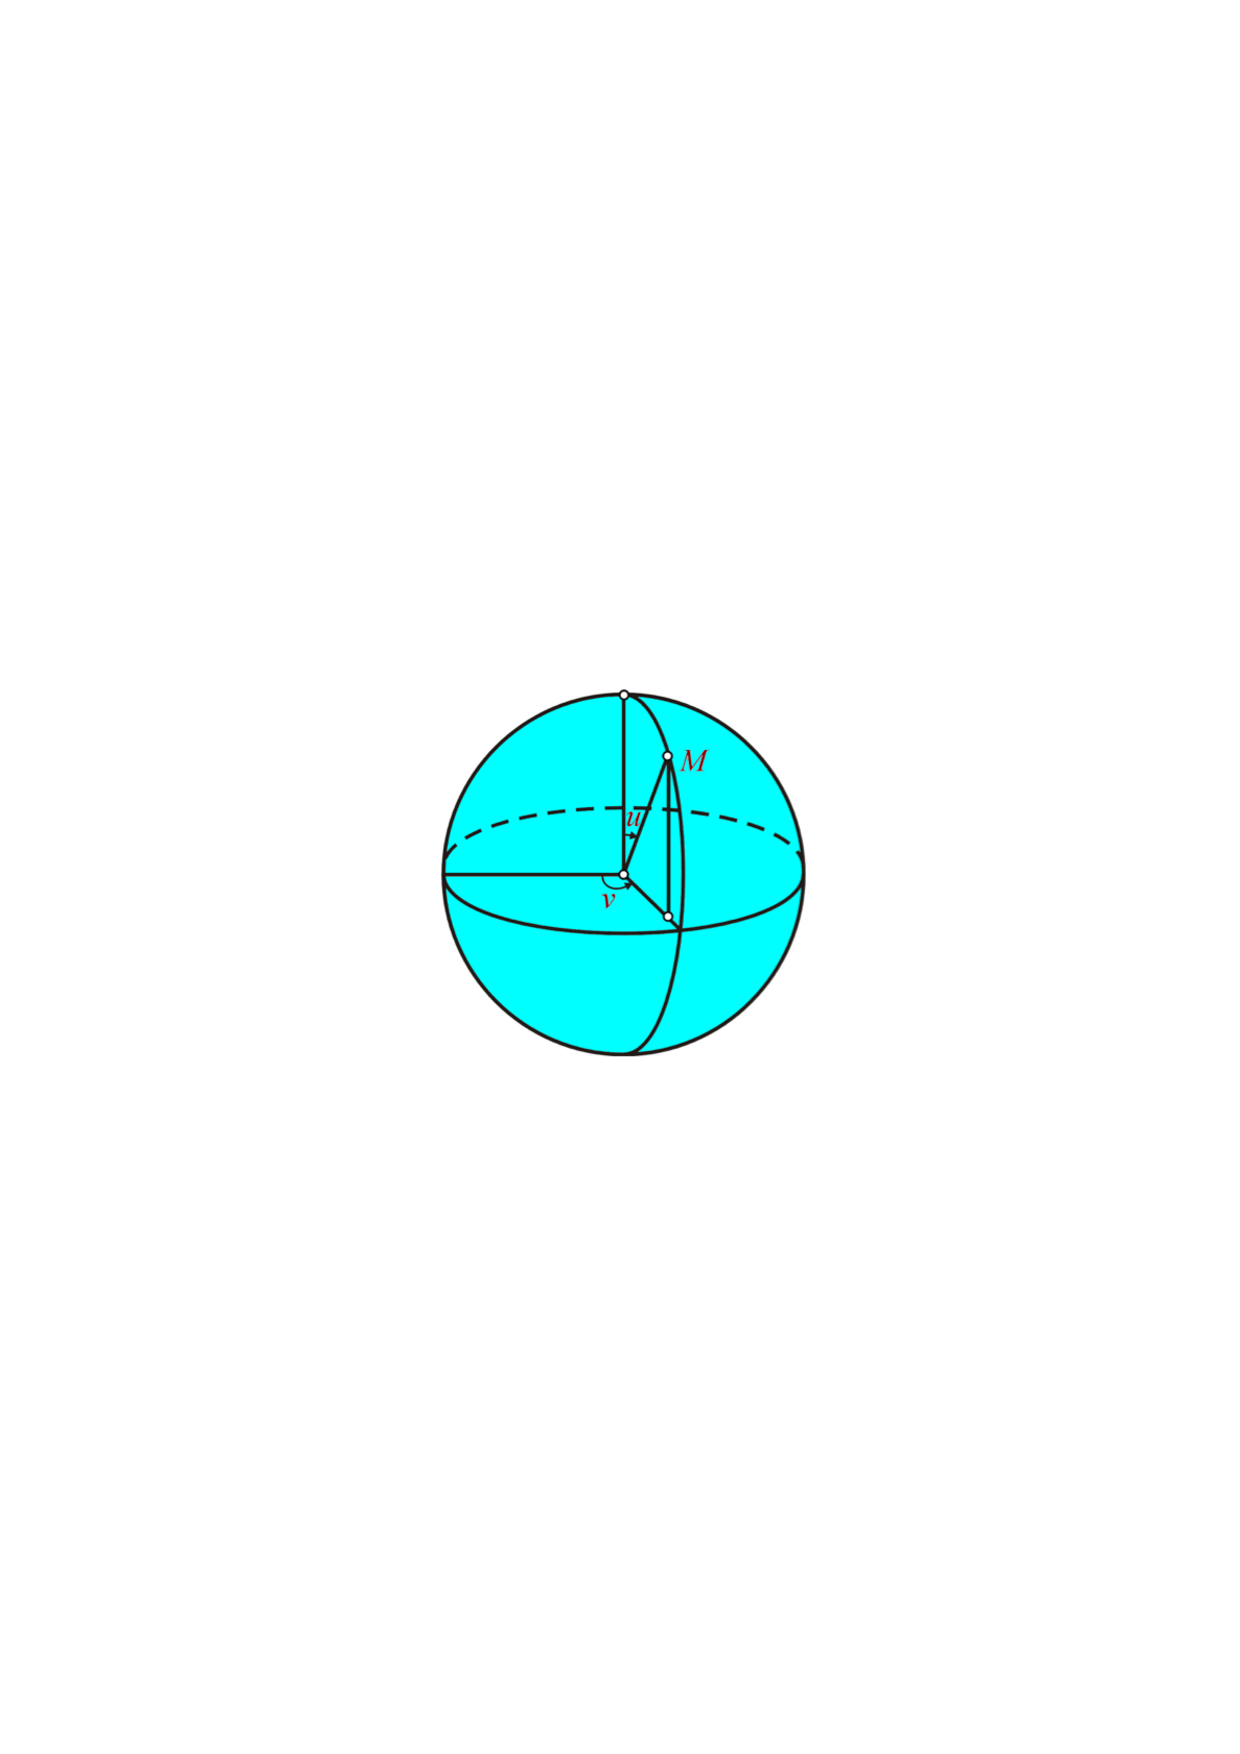
\includegraphics[scale = 0.6]{figs/sfera}
	\caption{Sfera în spațiul euclidian tridimensional}
\end{figure}

Expresia care apare în definiția sferei este un polinom de gradul doi în
nedeterminatele $x, y, z$, lucru care ne sugerează că ar trebui, în general,
să cercetăm mulțimea $\Sigma$ din $\mathbb{R}^3$, descrisă de o ecuație
de forma: 
 \[
	x^2 + y^2 + z^2 + 2ax + 2by + 2cz + d = 0.
\]

Această ecuație poate fi rescrisă ca: 
 \[
	(x + a)^2 + (y + b)^2 + (z + c)^2 = \rho = a^2 + b^2 + c^2 - d,
\]
numită \emph{ecuația carteziană generală} a sferei.

Rezultă din această descriere că:
\begin{enumerate}[(a)]
	\item Dacă $\rho > 0$, atunci $\Sigma$ este o sferă cu centrul în 
$(-a, -b, -c)$ și cu raza $\sqrt{\rho}$;
    \item Dacă $\rho = 0$, atunci $\Sigma = \{(-a, -b, -c)\}$;
    \item Dacă $\rho < 0$, atunci $\Sigma = \emptyset$.
\end{enumerate}

Ca suprafață din $\mathbb{R}^3$, sfera este o mulțime mărginită și închisă,
deci compactă. Ea separă spațiul în două submulțimi disjuncte, interiorul ei și
exteriorul ei. 

Dacă considerăm funcția: 
 \[
	f : \mathbb{R}^3 \to \mathbb{R},
	f(x, y, z) = (x - x_0)^2 + (y - y_0)^2 + (z - z_0)^2 - r^2,
\]
atunci cele două mulțimi pot fi descrise ca: 
 \[
	int(S) = \{(x, y, z) \mid f(x, y, z) < 0 \}, \quad
	ext(S) = \{(x, y, z) \mid f(x, y, z) > 0 \}.
\]

Două proprietăți topologice importante și totodată simple sînt:
\begin{theorem}
\begin{enumerate}[(a)]
	\item Mulțimea $int(S)$ este convexă.
	\item Pentru orice punct $M_1 \in int(S)$ și orice punct $M_2 \in ext(S)$,
segmentul $[M_1M_2]$ intersectează pe $S$.
\end{enumerate} 
\end{theorem}

Prin definiție, se numește \emph{plan tangent} la sferă în punctul 
$M_1(x_1, y_1, z_1)$ locul geometric al tuturor dreptelor tangente la sferă
în punctul $M_1$. O altă proprietate topologică a sferei, dedusă din definiția
ei cu ajutorul funcției de gradul al doilea, ne spune că ea este o suprafață
netedă, adică în fiecare punct al său există un plan tangent.

Ecuația planului tangent în punctul $M_1 \in S$ se obține prin dedublarea
ecuației sferei, adică: 
 \[
(x - x_0)(x_1 - x_0) + (y - y_0)(y_1 - y_0) + (z - z_0)(z_1 - z_0) - r^2 = 0,
\]
care poate fi prelucrată și rescrisă ca: 
 \[
	xx_1 + yy_1 + zz_1 + a(x + x_1) + b(y + y_1) + c(z + z_1) + d = 0.
\]

%%%%%%%%%%%%%%%%%%%%%%%%%%%%%%%%%%%%%%%%%%%%%%%%%%%%%%%%%%%%%%%%%%%%%%%%%%%%%%%%

\subsection{Elipsoidul}

\indent\indent Elipsoidul este o suprafață care generalizează sfera, la fel cum
elipsa este un caz mai general de cerc.

\begin{definition}

	Suprafața $\Sigma \seq \mathbb{R}^2$, de ecuație: 
 \[
	\dfrac{x^2}{a^2} + \dfrac{y^2}{b^2} + \dfrac{z^2}{c^2} - 1 = 0, a, b, c > 0
\]
se numește \emph{elipsoid.}
\end{definition}

Pentru a descrie forma geometrică a elipsoidului, îi studiem simetriile și
intersecțiile cu axele de coordonate, precum și cu plane paralele cu axele de
coordonate.

Dacă schimbăm oricare dintre nedeterminate cu opusa ei, ecuația elipsoidului
nu se schimbă. Așadar, un elipsoid este simetric față de planele de coordonate,
care se numesc \emph{plane principale} ale elipsoidului.


Totodată, suprafața este simetrică și față de axele de coordonate, care se 
numesc \emph{axele suprafeței}, deoarece schimbările tripletului $(x, y, z)$
în $(x, -y, -z)$ sau $(-x, y, -z)$ ori $(-x, -y, z)$ nu modifică ecuația 
elipsoidului. Rezultă de aici, în plus, că originea este un centru de simetrie.
Punctele în care axele de coordonate înțeapă suprafața elipsoidului se numesc
\emph{vîrfuri}.

Din ecuație, numerele $a, b, c$ se numesc \emph{semiaxe}. Intersecțiile
dintre planele de coordonate și elipsoid sînt elipse: 
 \[
	(1) \begin{cases}	
	         \dfrac{x^2}{a^2} + \dfrac{y^2}{b^2} - 1 &= 0 \\
	         z &= 0
        \end{cases}, \quad 
    (2) \begin{cases}	
           \dfrac{x^2}{a^2} + \dfrac{z^2}{c^2} - 1 &= 0 \\
           y &= 0
       \end{cases}, \quad 
    (3) \begin{cases}	
           \dfrac{y^2}{b^2} + \dfrac{z^2}{c^2} - 1 &= 0 \\
           x &= 0.
        \end{cases}
\]

Dacă intersectăm elipsoidul cu plane paralele cu $XOY$, obținem elipsele: 
 \[
	\begin{cases}	
	    \dfrac{x^2}{\frac{a^2}{c^2}(c^2 - k^2)} + 
	    \dfrac{y^2}{\frac{b^2}{c^2}(c^2 - k^2)} - 1 &= 0 \\
	    z &= k, k \in [-c, c]
    \end{cases}
\]
care sînt asemenea cu elipsa (1).

\begin{figure}[!h]
	\centering
	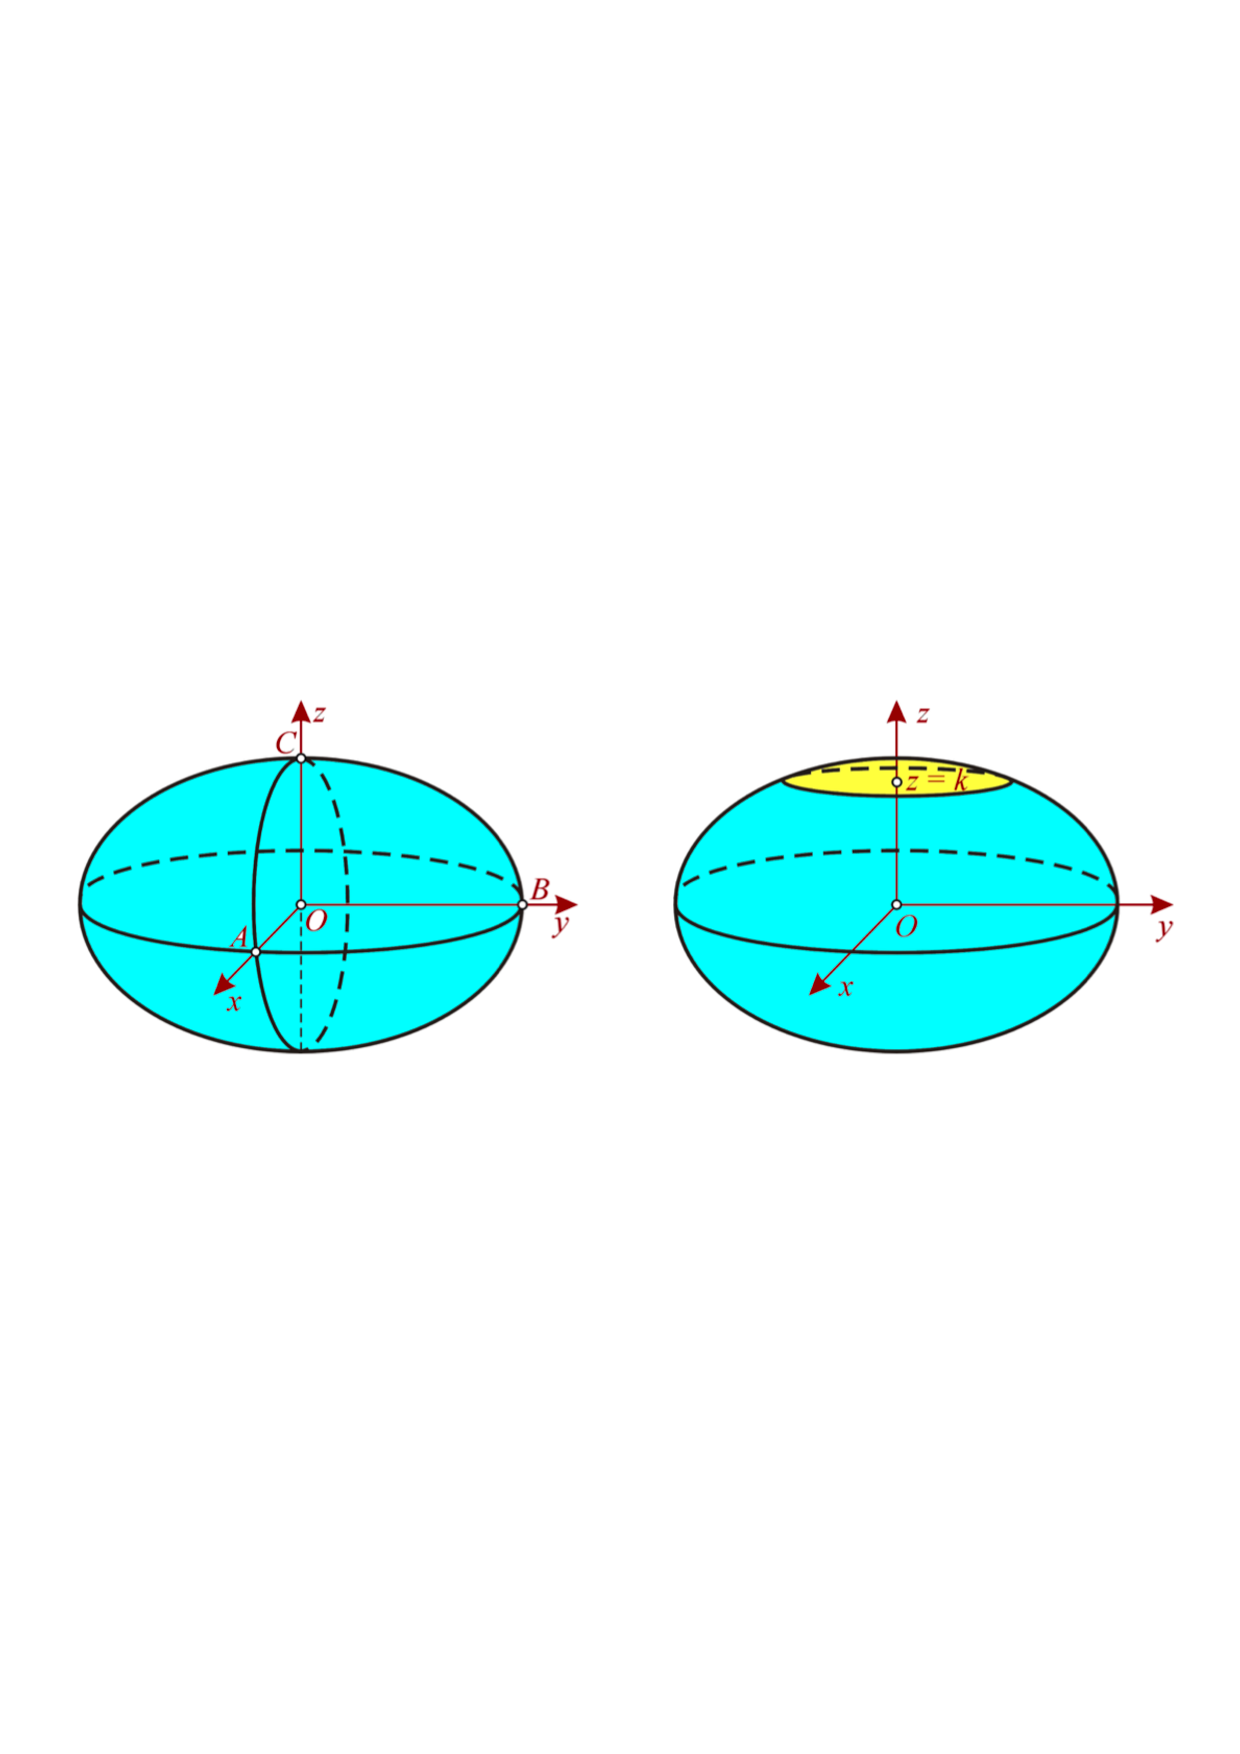
\includegraphics[scale = 0.6]{figs/elipse}
	\caption{Intersecția elipsoidului cu planele principale}
\end{figure}

O proprietate topologică importantă este:

\begin{theorem}
	Elipsoidul este o mulțime mărginită și închisă, deci compactă în spațiu.
\end{theorem}

\begin{proof}
	Din ecuația elipsoidului, deducem că toate rapoartele sînt subunitare, 
adică: 
 \[
	-a \leq x \leq a, \quad -b \leq y \leq b, \quad -c \leq z \leq c.
\]

Astfel, toate punctele elipsodului sînt cuprinse într-un paralelipiped cu 
laturile de lungimi finite. 

Elipsoidul $\Sigma$ este o mulțime închisă în spațiu, deoarece $\{1\}$ este 
închisă în $\mathbb{R}$, iar întreg elipsoidul poate fi privit ca imaginea 
inversă a lui $1$, prin funcția: 
 \[
	g : \mathbb{R}^3 \to \mathbb{R}, 
	g(x, y, z) = \dfrac{x^2}{a^2} + \dfrac{y^2}{b^2} + \dfrac{z^2}{c^2},
\]
care este o funcție continuă, deci întoarce închiși în închiși.
\end{proof}

De asemenea, avem și:

\begin{theorem}
	Intersecția dintre un elipsoid și un plan arbitrar este o elipsă, un punct
sau mulțimea vidă.
\end{theorem}

\begin{proof}
	Intersecția dintre un elipsoid și un plan este o curbă de gradul al doilea,
adică o conică. Deoarece elipsoidul este o mulțime compactă, fiind închisă și
mărginită, rezultă că intersecția trebuie să fie mărginită. Singurele conice
mărginite sînt elipsa, punctul și mulțimea vidă.
\end{proof}

%%%%%%%%%%%%%%%%%%%%%%%%%%%%%%%%%%%%%%%%%%%%%%%%%%%%%%%%%%%%%%%%%%%%%%%%%%%%%%%%

\subsection{Hiperboloizii}

\indent\indent Următoarea cuadrică de care ne ocupăm este \emph{hiperboloidul}.

Vom vedea că există două tipuri de hiperboloizi, de aceea referința este la
plural.

\begin{definition}
	Suprafața $\Sigma \seq \mathbb{R}^2$, de ecuație: 
 \[
	\dfrac{x^2}{a^2} + \dfrac{y^2}{b^2} - \dfrac{z^2}{c^2} - 1 = 0, a, b, c > 0
\]
se numește \emph{hiperboloid cu o pînză}.

\end{definition}

De remarcat, încă din ecuație, este faptul că această suprafață particulară are
aceleași simetrii ca și elipsoidul. Intersecțiile hiperboloidului cu planele
$x = 0$ și $y = 0$ sînt hiperbole: 
 \[
	\begin{cases}	
	    \dfrac{y^2}{b^2} - \dfrac{z^2}{c^2} - 1 &= 0 \\
	    x &= 0
    \end{cases}, \quad
    \begin{cases}	
	    \dfrac{x^2}{a^2} - \dfrac{z^2}{c^2} - 1 &= 0 \\
	    y &= 0.
    \end{cases}
\]

Dacă intersectăm suprafața cu plane de forma $z = k$, obținem elipse asemenea,
pentru orice $k \in \mathbb{R}$. Rezultă, așadar, forma din figura de mai jos.

\begin{figure}[!h]
	\centering
	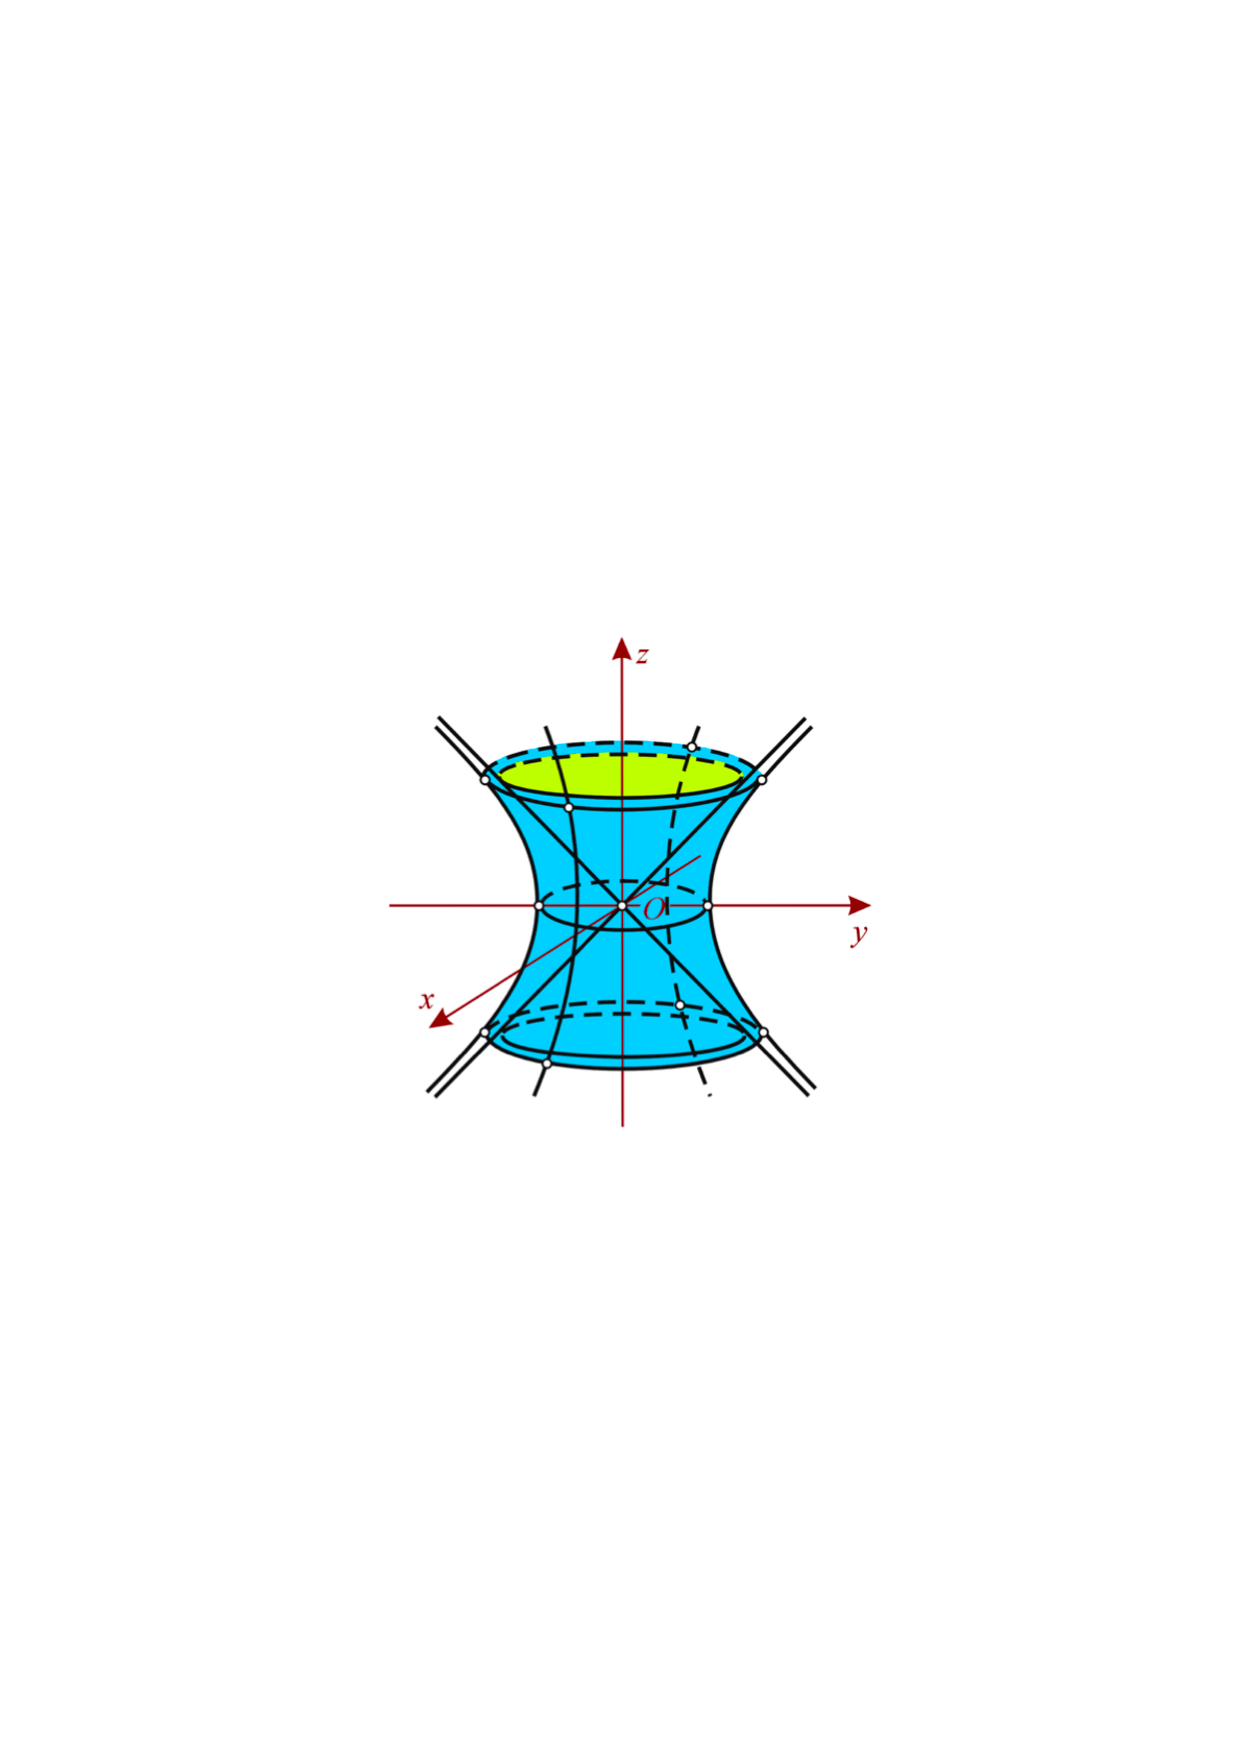
\includegraphics[scale = 0.6]{figs/hiperboloid1}
	\caption{Hiperboloidul cu o pînză}
\end{figure}

Se observă, din figură, că hiperboloidul cu o pînză este o mulțime nemărginită,
deoarece conține două hiperbole și închisă în $\mathbb{R}^3$.

\begin{definition}
	Suprafața $\Sigma \seq \mathbb{R}^3$, de ecuație: 
 \[
	\dfrac{x^2}{a^2} + \dfrac{y^2}{b^2} - \dfrac{z^2}{c^2} + 1 = 0, a, b, c > 0
\]
se numește \emph{hiperboloid cu două pînze}.

\end{definition}

Aceleași simetrii ca și în cazul hiperboloidului cu o pînză se pot remarca și
în acest caz. Hiperboloidul cu două pînze are două vîrfuri situate pe axa $OZ$,
iar intersecțiile sale cu planele $x = 0$ și $y = 0$ sînt hiperbolele: 
 \[
	\begin{cases}	
	    \dfrac{y^2}{b^2} - \dfrac{z^2}{c^2} + 1 &= 0 \\
	    x &= 0
    \end{cases}, \quad
    \begin{cases}	
	    \dfrac{x^2}{a^2} - \dfrac{z^2}{c^2} + 1 &= 0 \\
	    y &= 0
    \end{cases}
\]

În regiunea $-c < z < c$ nu avem puncte ale hiperboloidului, iar intersecția
suprafeței cu planele $z = k$, cu $|k| \geq c$ este dată de elipsele asemenea: 
 \[
	\begin{cases}	
	    \dfrac{x^2}{\frac{a^2}{c^2}(k^2 - c^2)} + 
	    \dfrac{y^2}{\frac{b^2}{c^2}(k^2 - c^2)} - 1 &= 0 \\
	    z &= k
    \end{cases}
\]

De asemenea, hiperboloidul cu două pînze este o mulțime nemărginită și închisă
în $\mathbb{R}^3$ și este schițat în figura de mai jos.

\begin{figure}[!h]
	\centering
	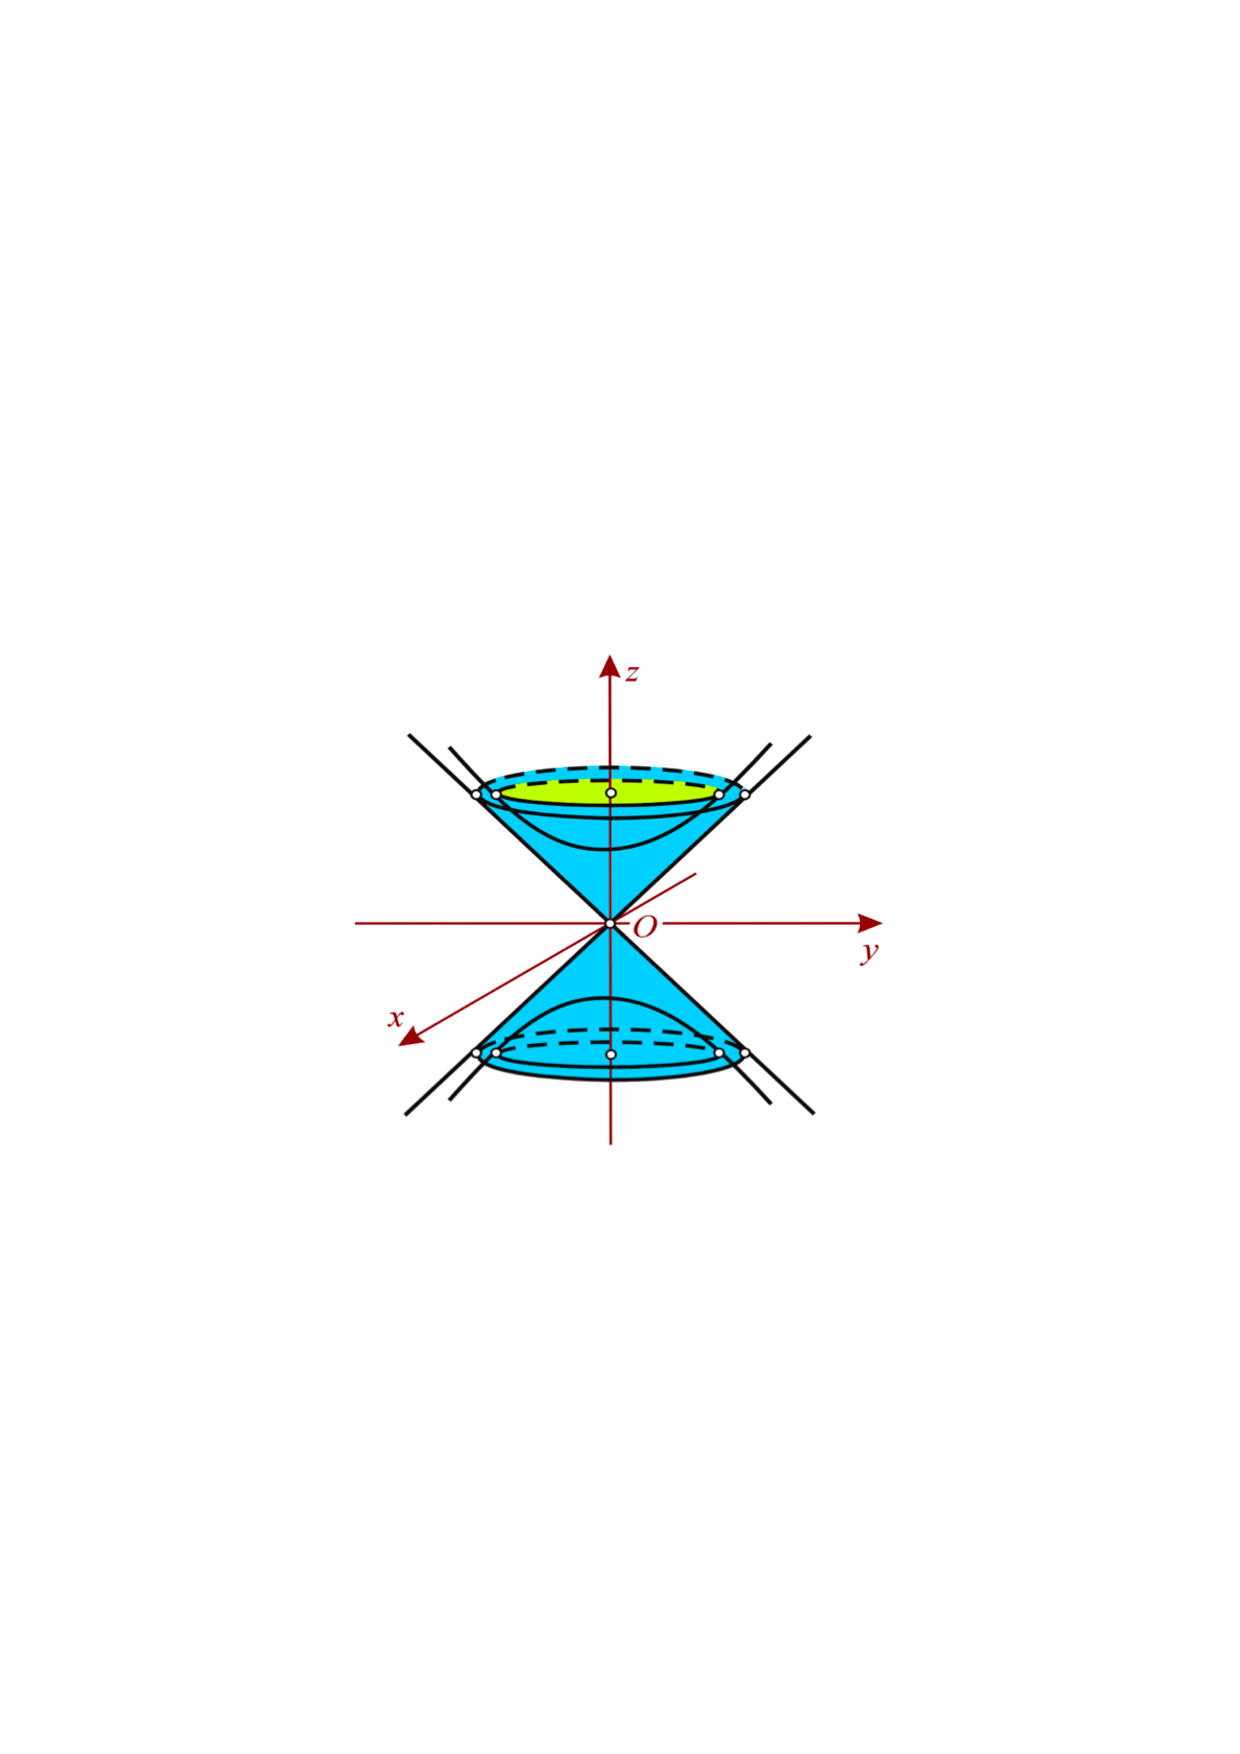
\includegraphics[scale = 0.6]{figs/hiperboloid2}
	\caption{Hiperboloidul cu două pînze}
\end{figure}

%%%%%%%%%%%%%%%%%%%%%%%%%%%%%%%%%%%%%%%%%%%%%%%%%%%%%%%%%%%%%%%%%%%%%%%%%%%%%%%%

\subsection{Paraboloizii}

\begin{definition}
	Suprafața $\Sigma \seq \mathbb{R}^3$, de ecuație: 
 \[
	z = \dfrac{x^2}{a^2} + \dfrac{y^2}{b^2}, a, b > 0
\]
se numește \emph{paraboloid eliptic}.

\end{definition}

Planele de simetrie $x = 0$ și $y = 0$ se numesc \emph{plane principale}. De
asemenea, remarcăm că $OZ$ este axă de simetrie și înțeapă suprafața în origine.
Punctul acesta se numește \emph{vîrf}, iar intersecțiile paraboloidului eliptic
cu planele $x = 0$ și $y = 0$ sînt parabolele: 
 \[
	\begin{cases}	
	    z &= \dfrac{y^2}{b^2} \\
	    x &= 0
    \end{cases}, \quad
    \begin{cases}	
	    z &= \dfrac{x^2}{a^2} \\
	    y &= 0.
    \end{cases}
\]

Rezultă că paraboloidul eliptic este o suprafață nemărginită. Evident, din 
ecuația de definiție se vede că paraboloidul eliptic există numai pentru
$z \geq 0$.

Intersecția paraboloidului cu planele $z = k > 0$ dă elipsele: 
 \[
	\begin{cases}	
	    \dfrac{x^2}{a^2} + \dfrac{y^2}{b^2} &= k \\
	    z &= k.
    \end{cases}
\]

Din aceste considerente, deducem că forma paraboloidului eliptic este ca
în figura de mai jos.

\begin{figure}[!h]
	\centering
	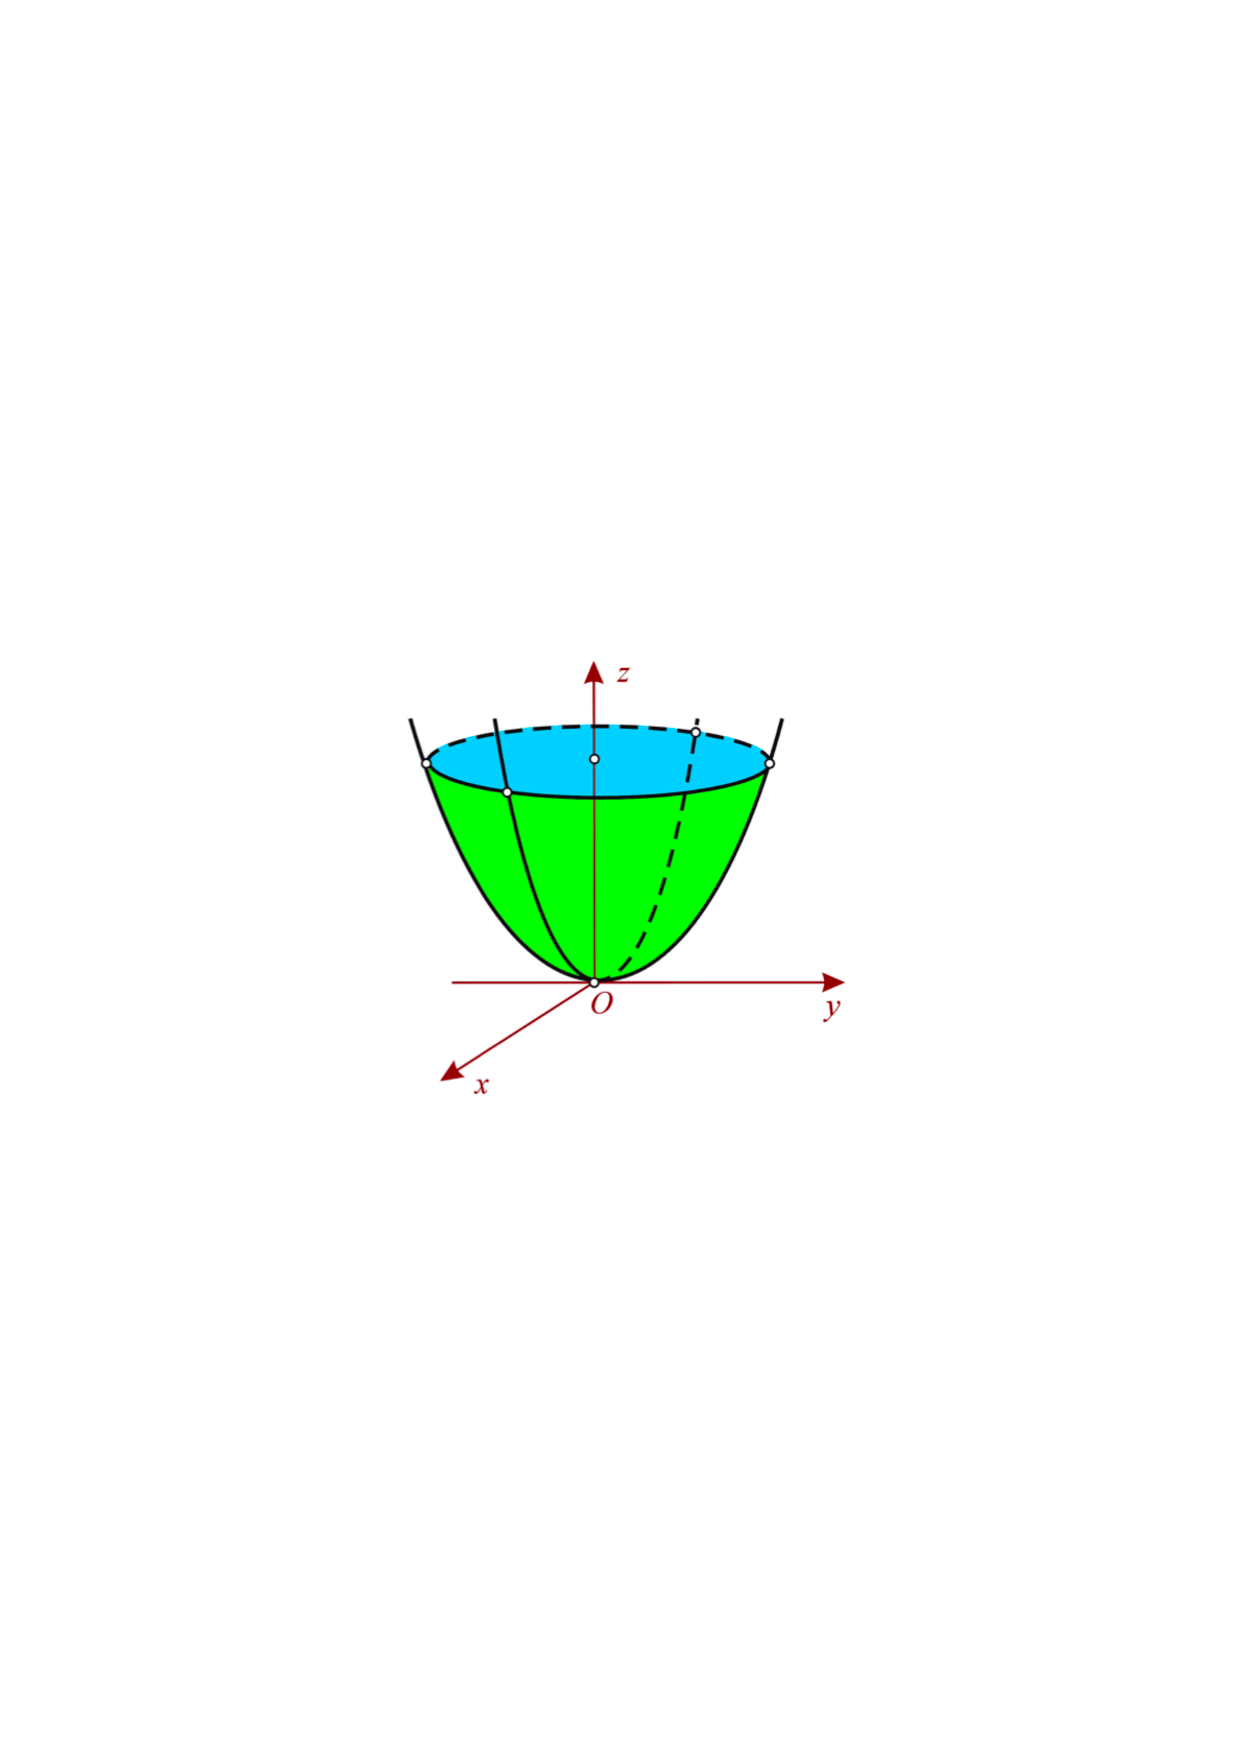
\includegraphics[scale = 0.6]{figs/paraboloid-eliptic}
	\caption{Paraboloidul eliptic}
\end{figure}

În cazul particular $a = b$, obține paraboloidul de rotație, care se obține prin
rotația unei parabole în jurul axei sale. Paraboloidul eliptic este o mulțime
nemărginită și închisă în $\mathbb{R}^3$.

\begin{definition}
	Suprafața $\Sigma$ de ecuație: 
 \[
	z = \dfrac{x^2}{a^2} - \dfrac{y^2}{b^2}
\]
se numește \emph{paraboloid hiperbolic} sau \emph{suprafață-șa}.

\end{definition}

Această suprafață are aceleași simetrii ca și paraboloidul eliptic. Originea
este vîrf al suprafeței, iar intersecția cu planul $x = 0$ dă parabola: 
 \[
	\begin{cases}	
	    z &= - \dfrac{y^2}{b^2} \\
	    x &= 0,
    \end{cases}
\]
care are concavitatea spre sensul negativ al axei $OZ$, deoarece $z \leq 0$.
Intersecția cu planul $y = 0$ ne dă parabola: 
 \[
	\begin{cases}	
	    z &= \dfrac{x^2}{a^2} \\
	    y &= 0,
    \end{cases}
\]
care are axa de simetrie $OZ$ și este dirijată în sensul pozitiv al acestei axe.

Dacă intersectăm suprafața cu planele $z = k > 0$, obținem hiperbolele: 
 \[
	\begin{cases}	
	    \dfrac{x^2}{a^2} - \dfrac{y^2}{b^2} &= k \\
	    z &= k,
    \end{cases}
\]
care au axa transversă paralelă cu $OX$.

Dacă intersectăm cu planele $z = k < 0$, obținem hiperbolele: 
 \[
	\begin{cases}	
	    \dfrac{x^2}{a^2} - \dfrac{y^2}{b^2} &= k \\
	    z &= k.
    \end{cases}
\]

Așadar, obținem forma din figura de mai jos.

\begin{figure}[!h]
	\centering
	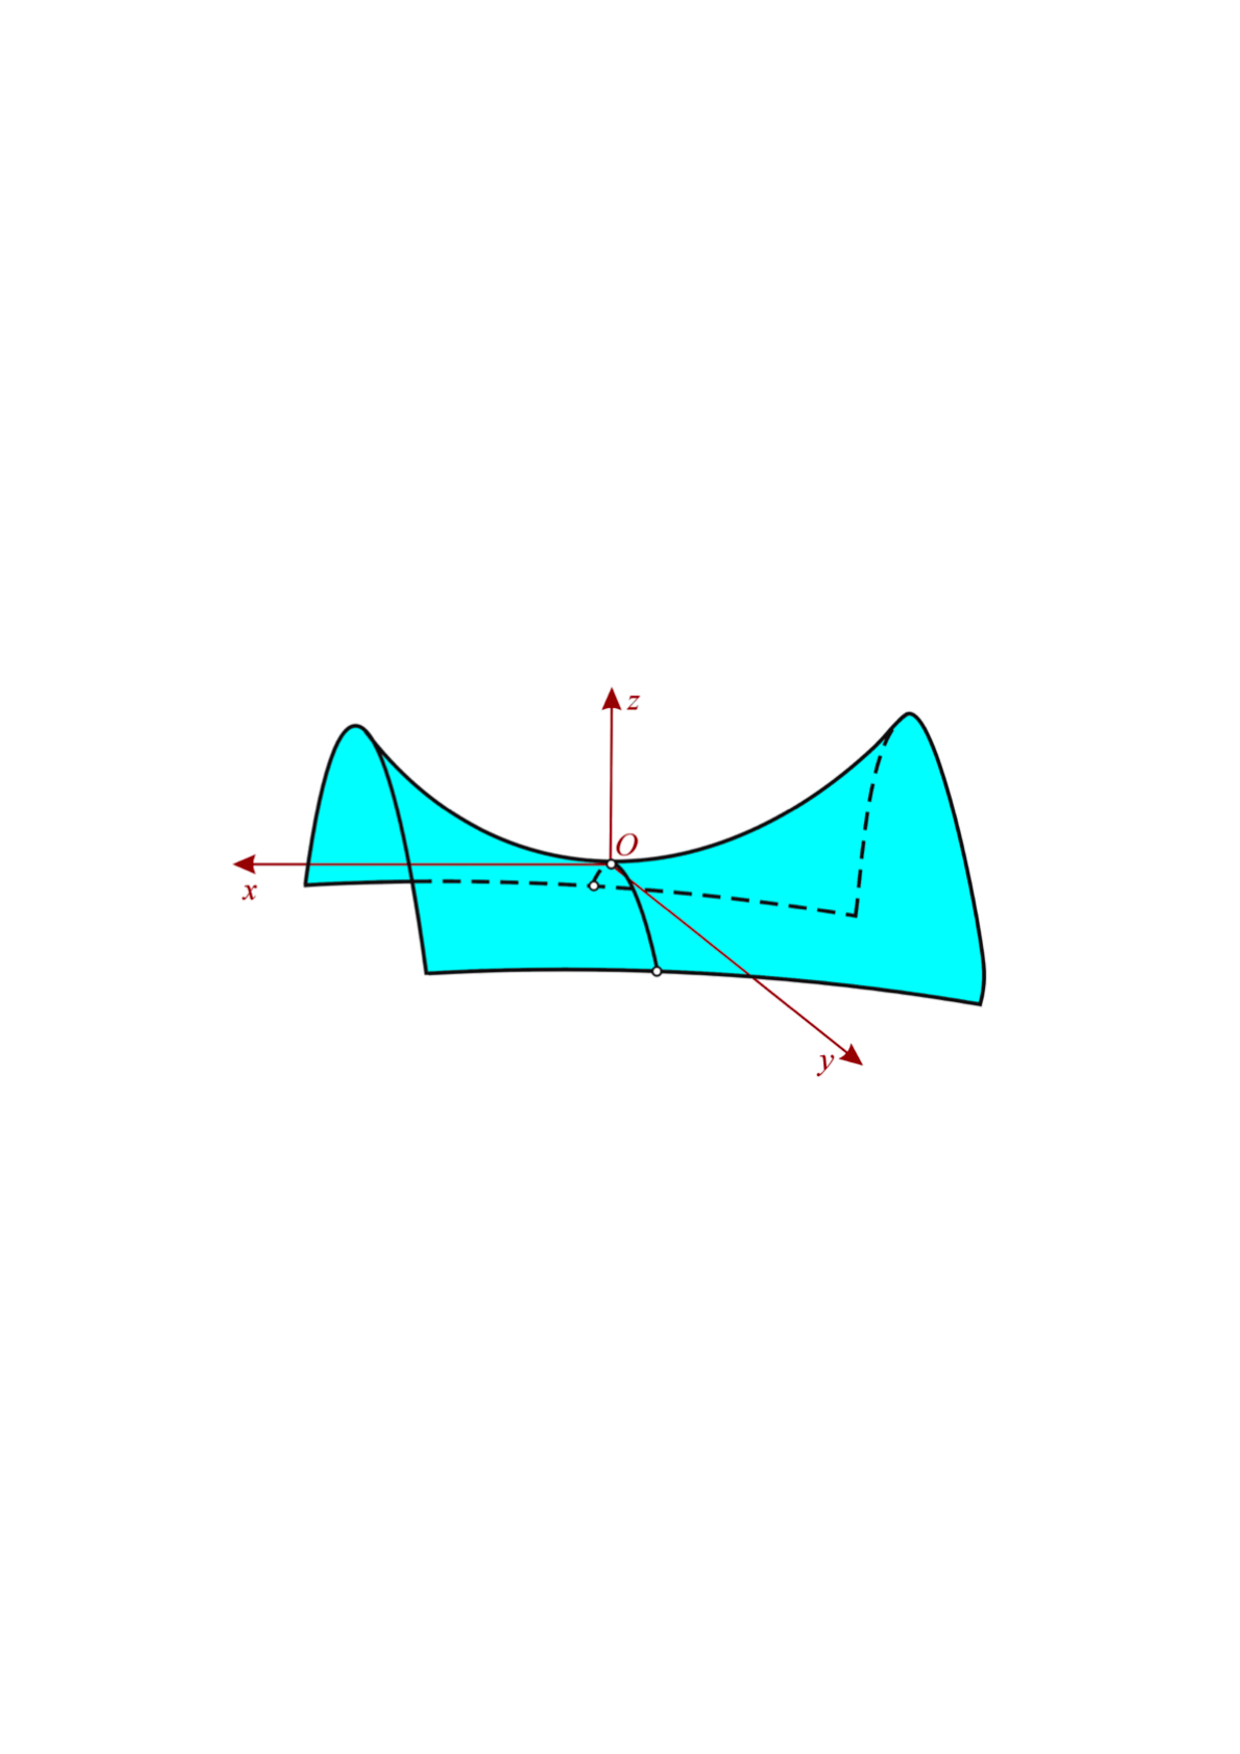
\includegraphics[scale = 0.6]{figs/paraboloid-hiperbolic}
	\caption{Paraboloidul hiperbolic (suprafață-șa)}
\end{figure}

Ca mulțime, suprafața este nemărginită și închisă.

%%%%%%%%%%%%%%%%%%%%%%%%%%%%%%%%%%%%%%%%%%%%%%%%%%%%%%%%%%%%%%%%%%%%%%%%%%%%%%%%

\subsection{Cilindri, perechi de plane}

\indent\indent În acest paragraf, completăm lista cuadricelor definite prin
ecuații canonice, cu cazurile speciale care au rămas.

Cuadrica de ecuație: 
 \[
    x^2 + y^2 - a^2 = 0
\]
se numește \emph{cilindru circular}. Un alt exemplu îl constituie cuadrica de 
ecuație: 
 \[
    \dfrac{x^2}{a^2} + \dfrac{y^2}{b^2} - 1 = 0,
\]
care se numește \emph{cilindru eliptic}.

În fine, cuadrica de ecuație: 
 \[
    \dfrac{x^2}{a^2} - \dfrac{y^2}{b^2} - 1 = 0
\]
se numește \emph{cilindru hiperbolic}, iar cuadrica de ecuație: 
 \[
    y^2 = 2px
\]
se numește \emph{cilindru parabolic}.


Alte tipuri speciale de cuadrice includ:
\begin{itemize}
    \item perechi de plane concurente, de ecuație: 
 \[
    \dfrac{x^2}{a^2} - \dfrac{y^2}{b^2} = 0;
\]
    \item perechi de plane paralele, de ecuație $x^2 - a^2 = 0$;
    \item perechi de plane confundate: $x^2 = 0$;
    \item dreapta (în spațiu): $\dfrac{x^2}{a^2} + \dfrac{y^2}{b^2} = 0$;
    \item punctul (în spațiu): 
$\dfrac{x^2}{a^2} + \dfrac{y^2}{b^2} + \dfrac{z^2}{c^2} = 0$;
    \item mulțimea vidă:
$\dfrac{x^2}{a^2} + \dfrac{y^2}{b^2} + \dfrac{z^2}{c^2} + 1 = 0$ sau
$\dfrac{x^2}{a^2} + \dfrac{y^2}{b^2} + 1 = 0$ sau 
$x^2 + a^2 = 0$, cu $a \neq 0$.
\end{itemize}

%%%%%%%%%%%%%%%%%%%%%%%%%%%%%%%%%%%%%%%%%%%%%%%%%%%%%%%%%%%%%%%%%%%%%%%%%%%%%%%%

\subsection{* Generatoare rectilinii}

\indent\indent În cele ce urmează, vom studia moduri în care o cuadrică poate fi
generată, prin diverse metode geometrice. De exemplu, vom vedea că unele cuadrice
pot fi generate prin mișcarea unei drepte sau prin mișcarea unor alte tipuri
de conice.

\begin{definition}
	O cuadrică $\Sigma$ care poate fi generată prin mișcarea unei drepte $D$
care se sprijină pe o curbă $C$ se numește \emph{cuadrică riglată}.

Dreapta $D$ se numește \emph{generatoarea rectilinie} a cuadricei riglate,
iar curba $C$ se numește \emph{curbă directoare}.

\end{definition}

Definiția poate fi reformulată fără a face uz de dreapta directoare. Într-adevăr,
putem numi o cuadrică \emph{riglată} dacă prin orice punct al său trece cel puțin
o dreaptă conținută în cuadrică.

O cuadrică se numește \emph{dublu riglată} dacă prin fiecare punct al său trec
două drepte distincte, care sînt conținute în cuadrică.


În ce privește cuadricele discutate pînă acum, avem:
\begin{theorem}
	Hiperboloidul cu o pînză și paraboloidul hiperbolic sînt cuadrice 
dublu riglate.
\end{theorem}

\begin{proof}
	Hiperboloidul cu o pînză are ecuația: 
 \[
	\Sigma_1 : \dfrac{x^2}{a^2} + \dfrac{y^2}{b^2} - \dfrac{z^2}{c^2} - 1 = 0.
\]

Această ecuație poate fi rescrisă ca: 
 \[
\Big(\dfrac{x}{a} - \dfrac{z}{c}\Big) \cdot \Big(\dfrac{x}{a} + 
\dfrac{z}{c}\Big) =\Big( 1 - \dfrac{y}{b} \Big) \cdot 
\Big( 1 - \dfrac{y}{b} \Big).
\]

Rezultă că avem următoarele familii de drepte incluse în hiperboloidul cu 
o pînză:
\begin{align*}
D_\lambda &: \begin{cases}
        \dfrac{x}{a} + \dfrac{z}{c} &= \lambda \Big( 1 + \dfrac{y}{b} \Big) \\
        \lambda \Big( \dfrac{x}{a} - \dfrac{z}{c} \Big) &= 1- \dfrac{y}{b}
    \end{cases}, \quad
D_\infty: \begin{cases}
			\dfrac{x}{a} - \dfrac{z}{c} &= 0 \\
			1 + \dfrac{y}{b} &= 0
		  \end{cases} \\
D_\mu &: \begin{cases}	
			\dfrac{x}{a} + \dfrac{z}{c} &= \mu \Big( 1 - \dfrac{y}{b} \Big) \\
			\mu \Big( \dfrac{x}{a} - \dfrac{z}{c} \Big) &= 1 + \dfrac{y}{b}
		\end{cases}, \quad
D^{\prime}_\infty : \begin{cases}
						\dfrac{x}{a} - \dfrac{z}{c} &= 0 \\
						1 - \dfrac{y}{b} &= 0.
\end{cases} 
\end{align*}

Mai mult, hiperboloidul poate fi obținut ca reuniune a acestor familii 
de drepte.

Cu alte cuvinte, familiile de mai sus sînt generatoare rectilinii ale
hiperboloidului cu o pînză.

Să remarcăm simplu că, dacă generatoarele rectilinii ale hiperboloidului cu
o pînză sînt translatate paralel în origine, atunci obținem generatoarele
rectilinii ale conului: 
 \[
	\Sigma: \dfrac{x^2}{a^2} + \dfrac{y^2}{b^2} - \dfrac{z^2}{c^2} = 0.
\]

Evident, de aici rezultă că conul este o suprafață simplu riglată.

Similar pentru paraboloidul hiperbolic: 
 \[
	\Sigma_2 : z = \dfrac{x^2}{a^2} - \dfrac{y^2}{b^2}
\]
poate fi generat de două familii de drepte. Pentru a găsi aceste familii
de drepte, transcriem ecuația paraboloidului hiperbolic în forma: 
 \[
	z = \Big( \dfrac{x}{a} - \dfrac{y}{b} \Big) \cdot 
		\Big( \dfrac{x}{a} + \dfrac{y}{b} \Big).
\]

De aici, rezultă că putem găsi familiile de drepte care sînt incluse în
paraboloidul hiperbolic:
\begin{align*}
	D_\lambda &: \begin{cases}	
					\dfrac{x}{a} + \dfrac{y}{b} &= \lambda z \\
					\lambda \Big( \dfrac{x}{a} - \dfrac{y}{b} \Big) &= 1
				\end{cases}, \quad
	D_\infty : \begin{cases}
					\dfrac{x}{a} - \dfrac{y}{b} &= 0 \\
					z &= 0
				\end{cases} \\
	D_\mu &: \begin{cases}	
				\dfrac{x}{a} - \dfrac{y}{b} &= \mu z \\
				\mu \Big( \dfrac{x}{a} + \dfrac{y}{b} \Big) &= 1
			\end{cases}, \quad
	D^{\prime}_\infty : \begin{cases}	
							\dfrac{x}{a} + \dfrac{y}{b} &= 0 \\
							z &= 0.
						\end{cases}
\end{align*}

Paraboloidul se realizează ca reuniunea acestor familii de drepte și avem
concluzia.

\end{proof}

Proprietățile esențiale ale familiilor de generatoare pentru cuadricele 
prezentate au următoarele proprietăți:

\begin{theorem}
	\textbf{Hiperboloidul cu o pînză}:
\begin{enumerate}[(a)]
	\item Orice două drepte din aceeași familie sînt necoplanare;
	\item O dreaptă din familia $D_\lambda$ și una din familia $D_\mu$
sînt coplanare;
	\item Oricare trei drepte din aceeași familie nu sînt paralele
cu același plan
\end{enumerate}

\textbf{Paraboloidul hiperbolic}:
\begin{enumerate}[(a)]
	\item Orice două drepte din aceeași familie sînt necoplanare;
	\item O dreaptă din familia $D_\lambda$ și una din familia $D_\mu$
sînt concurente;
    \item Oricare trei drepte din aceeași familie sînt paralele cu același plan.
\end{enumerate}
\end{theorem}

Proprietatea de a fi riglat poate fi extinsă și la suprafețe: o suprafață se
numește riglată dacă este generată prin mișcarea unei drepte $D$ care se 
sprijină pe o curbă $C$.

În acest caz, dacă generatoarea $D$ are ecuațiile parametrice: 
 \[
	\begin{cases}	
	    x &= x_0 + vl \\
	    y &= y_0 + vm \\
	    z &= z_0 + vn, v \in \mathbb{R},
    \end{cases}
\]
atunci suprafața riglată are ecuații parametrice de gradul 1 în $v$, adică: 
 \[
	\begin{cases}	
	    x &= x_0(u) + vl(u) \\
	    y &= y_0(u) + vm(u) \\
	    z &= z_0(u) + vn(u), (u,v) \in I \times \mathbb{R},
    \end{cases}
\]
unde $I$ este un interval convenabil din $\mathbb{R}$.

De remarcat este faptul că are loc și o reciprocă parțială a teoremei 
de mai sus:

\begin{theorem}
	Orice suprafață dublu riglată este un plan, un hiperboloid cu o pînză
sau un paraboloid hiperbolic.
\end{theorem}

\begin{proof}
	O suprafață riglată este dublu riglată dacă și numai dacă ecuațiile ei
parametrice sînt ecuații de gradul 1 în $v$ și de gradul $1$ în $u$, adică
arată: 
 \[
	\begin{cases}	
	    x &= a_0 + a_1 u + v(l_0 + l_1 u) \\
	    y &= b_0 + b_1 u + v(m_0 + m_1 u) \\
	    z &= c_0 + c_1 u + v(n_0 + n_1 u), (u, v) \in \mathbb{R}^2.
    \end{cases}
\]

Facem următoarea notație: 
 \[
	\Delta = \begin{vmatrix}
	             a_1 & l_0 & l_1 \\
	             b_1 & m_0 & m_1 \\
	             c_1 & n_0 & n_1
             \end{vmatrix}
\]

Se impune discuția: dacă $\Delta = 0$, atunci există $\alpha, \beta, \gamma$
numere reale, astfel încît: 
 \[
	\alpha (x - a_0) + \beta (y - b_0) + \gamma(z - c_0) = 0,
\]
ceea ce face ca suprafața studiată să fie un plan, care este o suprafață riglată
într-o infinitate de moduri.

Dacă $\Delta \neq 0$, atunci, prin eliminarea lui $u$ și $v$, obținem o ecuație
de gradul al doilea în $(x, y, z)$. În acest caz, suprafața dublu riglată este
o cuadrică, iar singurele cuadrice dublu riglate sînt hiperboloidul cu
o pînză și paraboloidul hiperbolic.
\end{proof}

%%%%%%%%%%%%%%%%%%%%%%%%%%%%%%%%%%%%%%%%%%%%%%%%%%%%%%%%%%%%%%%%%%%%%%%%%%%%%%%%

\subsection{Cuadrice descrise prin ecuația generală}

\indent\indent Descrierea analitică a cuadricelor invită la căutarea spațiului
pe care ecuația lor îl generează. Spațiul ambiant în care lucrăm este 
$\mathbb{R}^3$, dar vom căuta să identificăm mai precis spațiul corespunzător
cuadricelor prezentate prin ecuația generală.

Fie o formă pătratică afină $g : \mathbb{R}^3 \to \mathbb{R}$:
\begin{align*}
	g(x, y, z) = & a_{11}x^2 + a_{22}y^2 + a_{33}z^2 + \\
	            +& 2a_{12}xy + 2a_{13} xz + 2a_{23} yz + \\
	            +& 2a_{10}x + 2a_{20}y + 2a_{30} z \\
	            +& a_{00}.
\end{align*}

Cu aceasta, avem următoarea noțiune:
\begin{definition}
	Mulțimea de nivel constant zero: 
 \[
	\Sigma = \{ M(x, y, z) \in \mathbb{R}^3 \mid g(x, y, z) = 0\}
\]
se numește \emph{cuadrică} sau \emph{suprafață algebrică de ordinul al doilea}.

Aceasta se notează: $\Sigma: g(x, y, z) = 0$.
\end{definition}

Ca și în cazul conicelor, remarcăm că toate cuadricele sînt mulțimi închise
în spațiu, deoarece sînt imaginea inversă a lui $\{0\}$ -- care este mulțime
închisă -- printr-o funcție continuă, $g$, polinomială.

Ideea principală a secțiunii prezente și a celor ce vor urma este să vedem
moduri prin care o cuadrică poate fi adusă la forma canonică, identificînd
(sub)spații corespunzătoare în care această formă are loc. Așadar, se va trece
de la reperul cartezian standard $\{0, \vec{i}, \vec{j}, \vec{k}\}$ orientat
pozitiv la un alt reper față de care ecuația $g(x, y, z) = 0$ să aibă forma
cea mai simplă posibilă, care se va numi \emph{ecuația redusă (canonică)}.

Prin această transformare, se va arăta că mulțimea $\Sigma$ este congruentă cu
una din mulțimile: sferă, elipsoid, hiperboloid, paraboloid, con, cilindru,
pereche de plane, dreaptă, punct sau mulțime vidă.

Relativ la operațiile de rotație și translație pe care le vom face, cuadricele
au următorii invarianți:
\begin{align*}
	\Delta &= \det(\overline{A}), \quad \delta = \det(A) \\
	J &= \begin{vmatrix}
	         a_{11} & a_{12} \\
	         a_{21} & a_{22}
         \end{vmatrix} + 
         \begin{vmatrix}
	         a_{11} & a_{13} \\
	         a_{31} & a_{33} 
         \end{vmatrix} + 
         \begin{vmatrix}
	         a_{22} & a_{23} \\
	         a_{32} & a_{33}
         \end{vmatrix} \\
    I &= tr(A),
\end{align*}
unde matricele corespunzătoare sînt: 
 \[
	\overline{A} = \begin{pmatrix}
	                   a_{11} & a_{12} & a_{13} & a_{10} \\
	                   a_{21} & a_{22} & a_{23} & a_{20} \\
	                   a_{31} & a_{32} & a_{33} & a_{30} \\
	                   a_{01} & a_{02} & a_{03} & a_{00}
                   \end{pmatrix}, \quad
    A = \begin{pmatrix}
	        a_{11} & a_{12} & a_{13} \\
	        a_{21} & a_{22} & a_{23} \\
	        a_{31} & a_{32} & a_{33}
        \end{pmatrix},
\]
cu convenția pe care am mai folosit-o, anume $a_{ij} = a_{ji}, i \neq j$.

Acești invarianți vor fi folosiți pentru clasificarea cuadricelor. În primă
fază, vom avea:
\begin{itemize}
	\item Dacă $\Delta = 0$, atunci cuadrica este \emph{degenerată}, fiind o
reuniune de plane;  
    \item Dacă $\Delta \neq 0$, atunci cuadrica este nedegenerată.
\end{itemize}

Dintre cuadricele nevide, sfera, elipsoidul, hiperboloizii și paraboloizii
sînt cuadrice nedegenerate, iar conul, cilindrii și perechile de plane sînt
cuadrice degenerate.

În cazul sferei, avem o cuadrică pentru care $a_{11} = a_{22} = a_{33} = m$,
număr real nenul, iar $a_{12} = a_{13} = a_{23} = 0$, identificări care rezultă
din examinarea ecuației corespunzătoare. De asemenea: 
 \[
	\rho = \Big( \dfrac{a_{10}}{m} \Big)^2 + 
	        \Big( \dfrac{a_{20}}{m} \Big)^2 + 
	        \Big( \dfrac{a_{30}}{m} \Big)^2 -
	        \dfrac{a_{00}}{m} > 0.
\]

Centrul sferei este punctul: \[
	\Big( -\dfrac{a_{10}}{m}, - \dfrac{a_{20}}{m}, - \dfrac{a_{30}}{m} \Big),
\]
iar raza sferei este $r = \sqrt{\rho}$.

%%%%%%%%%%%%%%%%%%%%%%%%%%%%%%%%%%%%%%%%%%%%%%%%%%%%%%%%%%%%%%%%%%%%%%%%%%%%%%%%

\subsection{Centrul cuadricelor}

\indent\indent Ca în cazul conicelor, centrul de simetrie al unei cuadrice
este un punct critic al funcției $g$, adică este soluția sistemului liniar: 
 \[
	\begin{cases}	
	    \dfrac{1}{2} \dfrac{\partial g}{\partial x} &=
	    a_{11} x + a_{12}y + a_{13} z + a_{10} = 0 \\
	    \dfrac{1}{2} \dfrac{\partial g}{\partial y} &= 
	    a_{12} x + a_{22} y + a_{23} z + a_{20} = 0 \\
	    \dfrac{1}{2} \dfrac{\partial g}{\partial z} &= 
	    a_{13} x + a_{23}y + a_{33} z + a_{30} = 0/
    \end{cases}
\]

Discuția cazurilor posibile:

\begin{enumerate}[(1)]
	\item Dacă $\det(A) = \delta \neq 0$, atunci sistemul liniar de mai sus
este compatibil unic determinat. Așadar, cuadrica admite un singur centru
de simetrie la distanță finită. Acesta este cazul sferei, elipsoidului,
hiperboloizilor și conului;
    \item Dacă $\delta = 0$ și $\begin{pmatrix}
	                                a_{11} & a_{12} \\
	                                a_{12} & a_{22}
                                \end{pmatrix} \neq 0$,
și unicul determinant caracteristic al sistemului este nenul, atunci sistemul
este incompatibil. Cele trei plane reprezentate de cele trei ecuații formează
o prismă triunghiulară. Acesta este cazul paraboloidului eliptic și
paraboloidului hiperbolic.

    \item Dacă $\delta = 0$, iar determinantul de mai sus este nenul și
unicul determinant caracteristic este nul, sistemul liniar este compatibil
simplu nedeterminat.

Cele trei plane reprezentate de cele trei ecuații din sistem se intersectează
după o dreaptă numită \emph{dreaptă de centre}. Este cazul cilindrilor 
circulari, eliptici și hiperbolici.

    \item Dacă $\delta = 0$ și rangul sistemului este 1, iar cei doi 
determinanți caracteristici sînt nenuli, atunci sistemul este incompatibil

Obținem două plane paralele, care este cazul cilindrului parabolic.

    \item Dacă $\delta = 0$, rangul sistemului este 1, iar cei doi
determinanți caracteristici sînt nuli, atunci sistemul este compatibil dublu
nedeterminat. Obținem trei plane confundate, iar cuadrica are un plan de centre.

Este cazul planelor paralele distincte sau confundate.
\end{enumerate}

Să vedem un exemplu.

\begin{example}
	Fie cuadrica $\Sigma$, care conține două puncte, $A(-1, 2, 3)$ și
$B(1, 1, -1)$, precum și axa $OY$ și cercul $\Gamma$ cu centrul în 
$C(0, 0, 3)$, fiind tangent axei $OX$ în origine.

Vom scrie ecuația cuadricei, îi determinăm invarianții și coordonatele 
centrului.

Cercul $\Gamma$ se află în planul $XOZ$ și are ecuațiile: 
 \[
	x^2 + z^2 - 6z = 0, \quad y = 0.
\]

Atunci ecuația cuadricei are forma: 
 \[
	x^2 + z^2 - 6z + y(\alpha x + \beta y + \gamma z + \delta) = 0,
\]
deoarece intersecția dintre această suprafață și planul $XOZ$ este cercul
$\Gamma$.

Deoarece cuadrica conține axa $OY$, ecuația ei este identitatea pentru $z = 0$
și $x = 0$, de unde rezultă că $\beta = \delta = 0$.

Condițiile $A \in \Sigma$ și $B \in \Sigma$ conduc la sistemul: 
 \[
	\begin{cases}	
	    \alpha - 3 \gamma &= 4 \\
	    \alpha + \gamma &= 8
    \end{cases} \Longrightarrow \alpha = 7, \gamma = 1.
\]

Obținem, în fine: 
 \[
	\Sigma : x^2 + z^2 + 7xy + yz - 6z = 0.
\]

Invarianții corespunzători sînt: 
 \[
	\Delta = \begin{vmatrix}
	             1 & \frac{7}{2} & 0 & 0 \\
	             \frac{7}{2} & 0 & \frac{1}{2} & 0 \\
	             0 & \frac{1}{2} & 1 & -3 \\
	             0 & 0 & -3 & 0
             \end{vmatrix} = \dfrac{441}{4}.
\]

Rezultă că avem o cuadrică nedegenerată. Mai departe, $\delta = -\dfrac{25}{2}$,
deci cuadrica are un centru și $J = - \dfrac{23}{2}$, iar $I = 2$.

Centrul se află rezolvînd sistemul: 
 \[
	\begin{cases}	
	    2x + 7y &= 0 \\
	    7x + z &= 0 \\
	    2z + y - 6 &= 0.
    \end{cases}
\]
\end{example}

%%%%%%%%%%%%%%%%%%%%%%%%%%%%%%%%%%%%%%%%%%%%%%%%%%%%%%%%%%%%%%%%%%%%%%%%%%%%%%%%

\subsection{(!) Reducerea la forma canonică}

\indent\indent Vrem să stabilim ecuația canonică a unei cuadrice. Procedăm
astfel:
\begin{enumerate}[(a)]
	\item Dacă $a_{12} = a_{13} = a_{23} = 0$, atunci facem o translație și
eventual o rotație;
    \item Dacă cel puțin unul dintre numerele $a_{12}, a_{13}, a_{23}$ este
nenul, atunci tipul cuadricei este determinat de forma pătratică: 
 \[
	a_{11} x^2 + a_{22} y^2 + a_{33} z^2 + 2a_{12} xy + 2a_{13} xz + 2a_{23}yz.
\]

Considerăm matricea (simetrică) atașată acestei forme pătratice, căreia îi
determinăm valorile proprii, care sînt reale, precum și vectorii proprii
corespunzători, care sunt ortogonali sau pot fi făcuți astfel. Prin urmare,
obținem versorii $\vec{e}_1, \vec{e}_2, \vec{e_3}$.

Fie $R$ matricea formată de coordonatele acestor versori, aranjate pe coloane.
Putem presupune, eventual după o renumerotare sau înlocuirea unuia dintre 
versori cu opusul său, că $\det(R) = 1$. Atunci: 
 \[
	\begin{pmatrix}
	    x \\ y \\ z
    \end{pmatrix} = R \cdot \begin{pmatrix}
	                            x^{\prime} \\ y^{\prime} \\ z^{\prime}
                            \end{pmatrix}
\]
reduce forma pătratică la expresia canonică: 
 \[
\lambda_1 {x^{\prime}}^2 + \lambda_2 {y^{\prime}}^2 + \lambda_3 {z^{\prime}}^2.
\]

Mai departe, direcțiile noilor axe de coordonate sînt date de direcțiile 
versorilor proprii $\vec{e}_1, \vec{e}_2, \vec{e_3}$. Dacă este cazul, la final
se poate face o translație.
\end{enumerate}

Să vedem acestea aplicate pe un exemplu.

\begin{example}
	Se dă ecuația: 
 \[
	x^2 + y^2 + 5z^2 - 6xy + 2xz - 2yz - 4x + 8y - 12z + 14 = 0.
\]

Vrem să o reducem la forma canonică și să construim cuadrica corespunzătoare.

Considerăm forma pătratică asociată: 
 \[
	q(x, y, z) = x^2 + y^2 + 5z^2 - 6xy + 2xz - 2yz.
\]

Aceasta are matricea asociată: 
 \[
	A = \begin{pmatrix}
	        1 & -3 & 1 \\
	        -3 & 1 & -1 \\
	        1 & -1 & 5
        \end{pmatrix}
\]

Matricea are valorile proprii reale și distincte, $\lambda_1 = -2$,
$\lambda_2 = 3, \lambda_3 = 6$. Vectorii proprii corespunzători vor fi 
ortogonali, deoarece matricea $A$ este simetrică și are valori proprii 
distincte.

Versorii proprii obținuți vor fi: 
 \[
\begin{cases}
\vec{e}_1 &= \Big( \dfrac{1}{\sqrt{2}}, \dfrac{1}{\sqrt{2}}, 0 \Big) \\
\vec{e}_2 &= \Big( -\dfrac{1}{\sqrt{3}}, \dfrac{1}{\sqrt{3}},
                    \dfrac{1}{\sqrt{3}} \Big) \\
\vec{e}_3 &= \Big( \dfrac{1}{\sqrt{6}}, - \dfrac{1}{\sqrt{6}},
                \dfrac{2}{\sqrt{6}} \Big).
\end{cases}
\]

Matricea ortogonală $R$, ale cărei coloane sînt formate din componentele
versorilor proprii are determinantul $1$. Facem, atunci, rotația: 
 \[
	\begin{pmatrix}
	    x \\ y \\ z
    \end{pmatrix} = R \cdot \begin{pmatrix}
	                            x^{\prime} \\ y^{\prime} \\ z^{\prime}
                            \end{pmatrix}
\]

Astfel, ecuația carteziană generală devine: 
 \[
	-2{x^{\prime}}^2 + 3 {y^{\prime}}^2 + 6 {z^{\prime}}^2 +
	\dfrac{4}{\sqrt{2}} x^{\prime} - \dfrac{36}{\sqrt{6}}z^{\prime} + 14 = 0.
\]

Completăm pătratele și forțăm factorii comuni, obținînd: 
 \[
	-2 \Big( x^{\prime} - \dfrac{1}{\sqrt{2}} \Big)^2 + 3 {y^{\prime}}^2 + 
	6 \Big( z^{\prime} - \dfrac{3}{\sqrt{6}} \Big)^2 + 6 = 0.
\]

Facem, atunci, translația, în fine: 
 \[
	x^{\prime} = \dfrac{1}{\sqrt{2}} + x^{\prime\prime}, \quad
	y^{\prime} = y^{\prime\prime}, \quad 
	z^{\prime} = \dfrac{3}{\sqrt{6}} + z^{\prime\prime}
\]
și obținem ecuația canonică a unui hiperboloid cu două pînze, ale cărui
vîrfuri se află pe axa absciselor $CX^{\prime\prime}$: 
 \[
	- \dfrac{{x^{\prime\prime}}^2}{3} + 
	\dfrac{{y^{\prime\prime}}^2}{2} + 
	\dfrac{{z^{\prime\prime}}^2}{1} + 1 = 0.
\]

Reprezentarea geometrică este redată în figura 
\ref{figure:hiperboloid-exercitiu}:
\begin{figure}[!h]
	\centering
	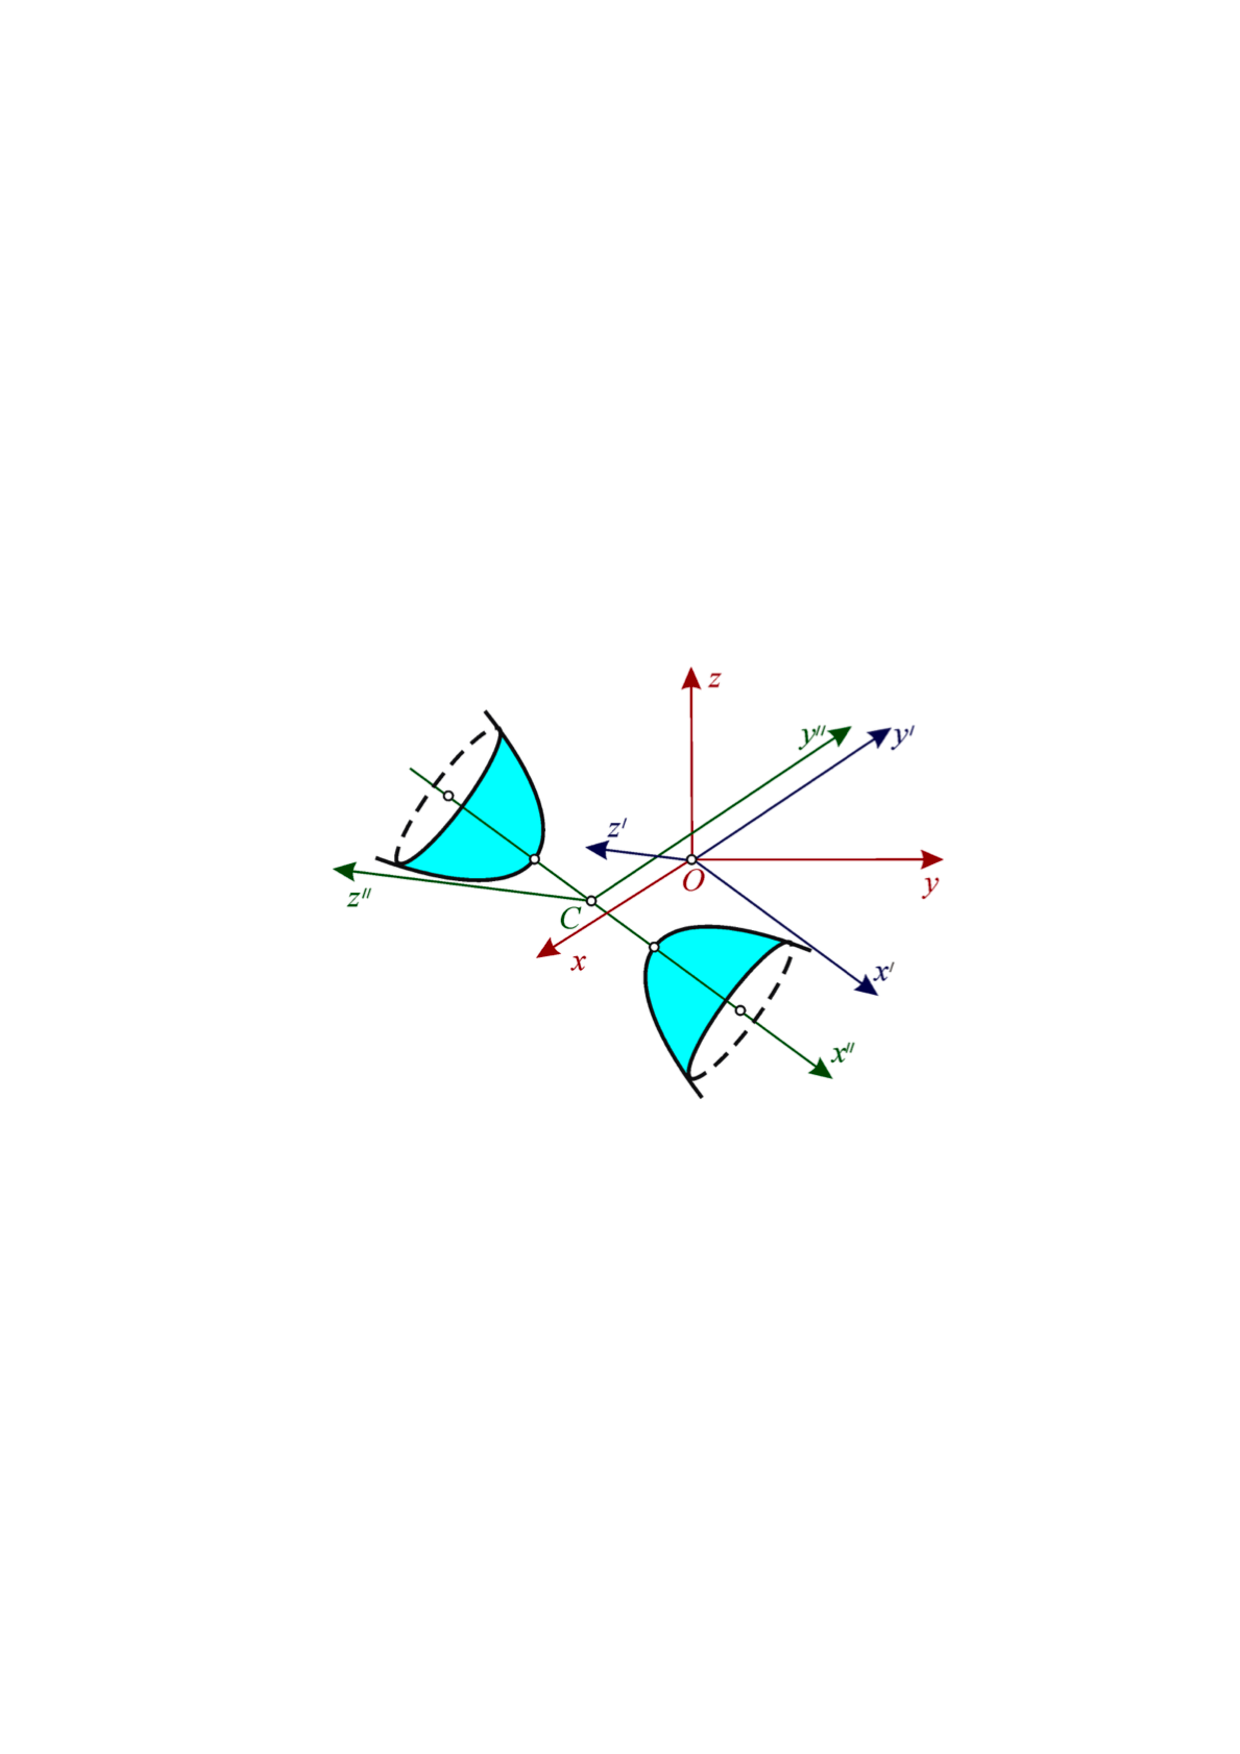
\includegraphics[scale = 0.6]{figs/hiperboloid-exercitiu}
	\caption{Hiperboloidul cu 2 pînze din exemplu}
    \label{figure:hiperboloid-exercitiu}
\end{figure}

\end{example}

%%%%%%%%%%%%%%%%%%%%%%%%%%%%%%%%%%%%%%%%%%%%%%%%%%%%%%%%%%%%%%%%%%%%%%%%%%%%%%%%

\subsection{Intersecția cu o dreaptă sau un plan}

\indent\indent Ca în cazul conicelor, studiem cazurile corespunzătoare
intersecțiilor între o cuadrică și o dreaptă sau un plan.

Fie, așadar, $D$ o dreaptă în spațiu de ecuații parametrice: 
 \[
	\begin{cases}	
	    x &= x_0 + lt \\
	    y &= y_0 + mt \\
	    z &= z_0 + nt, t \in \mathbb{R},
    \end{cases}
\]
precum și o cuadrică $\Sigma$ de ecuație generală $g(x, y, z) = 0$.

Intersecția $D \cap \Sigma$ corespunde rădăcinilor ecuației reale: 
 \[
	t^2 \varphi(l, m, n) + t(l g_{x_0} + mg_{y_0} + ng_{z_0}) + 
	g(x_0, y_0, z_0) = 0,
\]
unde am introdus funcția: 
 \[
	\varphi(l, m, n) = a_{11} l^2 + a_{22} m^2 + a_{33}n^2 +
	                  2a_{12}lm + 2a_{13}ln + 2a_{23}mn,
\]
iar $g_{x_0} = g_x(x_0, y_0, z_0)$ ș.cl.

Cazurile pe care le distingem sînt următoarele:

\begin{enumerate}[(1)]
	\item Dacă $\varphi(l, m, n) \neq 0$, atunci ecuația corespunzătoare
este o ecuație de gradul 2. Introducem notația pentru discriminant: 
 \[
	q = (lg_{x_0} + mg_{y_0} + ng_{z_0})^2 - 
	    4\varphi(l, m, n)g(x_0, y_0, z_0) > 0,
\]
de unde deducem că ecuația are două rădăcini reale distincte, $t_1$ și $t_2$.

Astfel, rezultă că dreapta $D$ intersectează cuadrica în două puncte, $M_1$ și
$M_2$. 

Dacă $q = 0$, atunci $t_1 = t_2$. În acest caz, $D$ intersectează $\Sigma$ în
două puncte confundate, caz în care dreapta $D$ se numește \emph{tangentă} la
$\Sigma$.

Dacă $q < 0$, atunci ecuația nu are rădăcini reale, deci $D$ nu intersectează
pe $\Sigma$.

    \item Dacă $\varphi(l, m, n) = 0$, atunci ecuația devine una de gradul
    întîi, pentru care discuția este mai simplă. Dacă $lg_{x_0} + mg_{y_0} +
ng_{z_0} \neq 0$, atunci avem o soluție unică, deci $D$ intersectează
cuadrica $\Sigma$ într-un singur punct.

Dacă $lg_{x_0} + mg_{y_0} + ng_{z_0} = 0$, dar $g(x_0, y_0, z_0) \neq 0$, atunci
ecuația nu are soluții. În acest caz, dreapta $D$ nu intersectează cuadrica
$\Sigma$.

Dacă $lg_{x_0} + mg_{y_0} + ng_{z_0} = 0$ și $g(x_0, y_0, z_0) = 0$, atunci
ecuația este o identitate și $D \seq \Sigma$.

\end{enumerate}

Fie $M(x_0, y_0, z_0) \in \Sigma$ un punct pentru care cel puțin unul din
numerele $g_{x_0}, g_{y_0}, g_{z_0}$ este nenul. Această ipoteză este folosită
implicit în rezultatele care urmează.

\begin{theorem}
	Dreapta $D$, de parametri directori $(l, m, n)$ este tangentă la cuadrica
$\Sigma$ în punctul $M(x_0, y_0, z_0) \in \Sigma$ dacă și numai dacă
$lg_{x_0} + mg_{y_0} + ng_{z_0} = 0$.
\end{theorem}

Justificarea a fost deja descrisă în cazurile analizate mai sus.

\begin{theorem}
	Locul geometric al tuturor tangentelor la cuadrica $\Sigma$ în punctul
$M_0 \in \Sigma$ este planul de ecuație: 
 \[
	(x - x_0)g_{x_0} + (y - y_0)g_{y_0} + (z - z_0) g_{z_0} = 0.
\]

Acest plan se numește \emph{planul tangent} la cuadrica $\Sigma$ în punctul
$M_0$.
\end{theorem}

De remarcat faptul că ecuația planului tangent într-un punct $M_0 \in \Sigma$
se poate obține și prin dedublarea ecuației $g(x, y, z) = 0$ în punctul $M_0$.
Cu aceasta, ecuația planului tangent este:
\begin{align*}
	& a_{11} xx_0 + a_{22} yy_0 + a_{33}zz_0 + a_{12}(x_0y + xy_0) +
	    a_{13}(x_0z + xz_0) + a_{23}(y_0 z+ yz_0) \\
	&+ a_{10}(x + x_0) + a_{20}(y + y_0) + a_{30}(z + z_0) + a_{00} = 0.
\end{align*}

Ca în cazul conicelor, cuadrica $\Sigma$ se numește \emph{netedă} dacă în
fiecare punct al său există un plan tangent. Netezimea cuadricei $\Sigma$
elimină punctele critice, adică acele puncte în care $g_x, g_y, g_z, g$ se
anulează simultan (e.g. vîrful unui con).

Dreapta care trece prin $M_0 \in \Sigma$ și este perpendiculară pe planul
tangent se numește \emph{normala la $\Sigma$} în $M_0$ și are ecuațiile: 
 \[
	\dfrac{x - x_0}{g_{x_0}} = \dfrac{y - y_0}{g_{y_0}} =
	\dfrac{z - z_0}{g_{z_0}}
\]

Intersecția dintre un plan $P: ax + by + cz + d = 0$ și o cuadrică oarecare
$\Sigma: g(x, y, z) = 0$ este descrisă de sistemul anulărilor lor simultane.

Dacă $c \neq 0$, atunci $z = \alpha x + \beta y + \gamma$ și înlocuim în
ecuația cuadricei. Astfel, intersecția $P \cap \Sigma$ se reduce la intersecția
dintre planul $P$ și cilindrul de gradul doi, de ecuație
$g(x, y, \alpha x + \beta y + \gamma) = 0$, care are generatoarele paralele
cu axa $OZ$; deci $P \cap \Sigma$ este o conică $\Gamma$.

Proiecția acestei conice $\Gamma = P \cap \Sigma$ pe planul $XOY: z = 0$ este o 
conică $\Gamma^{\prime}$, descrisă de sistemul: 
 \[
	\begin{cases}	
	    z &= 0\\
	    g(x, y, \alpha x + \beta y + \gamma) &= 0
    \end{cases}
\]

%%%%%%%%%%%%%%%%%%%%%%%%%%%%%%%%%%%%%%%%%%%%%%%%%%%%%%%%%%%%%%%%%%%%%%%%%%%%%%%%

\subsection{Exerciții rezolvate}

1. Se dă cuadrica: 
 \[
	\Sigma_1 : x^2 - y^2 + z^2 - 2xy - 2yz - 2zx - 5x - 1 = 0.
\]

\begin{enumerate}[(a)]
	\item Calculați invarianții $\Delta, \delta, J, I$;
	\item Aflați centrul de simetrie al cuadricei;
	\item Aduceți cuadrica la forma canonică folosind metoda rotațiilor și
translațiilor; obțineți matricea de rotație folosind metoda valorilor proprii.
\end{enumerate}

\emph{Soluție:}
(a)	Forma pătratică asociată este: 
 \[
	g(x, y, z) = x^2 - y^2 + z^2 - 2xy - 2yz - 2zx.
\]

Matricea formei pătratice este: 
 \[
	A = \begin{pmatrix}
	        1 & -1 & -1 \\
	        -1 & -1 & -1 \\
	        -1 & -1 & 1
        \end{pmatrix}
\]

Invarianții cuadricei sînt:
\begin{align*}
	\Delta &= \begin{vmatrix}
	             1 & -1 & -1 & -\frac{5}{2} \\
	             -1 & -1 & -1 & 0 \\
	             -1 & -1 & 1 & 0 \\
	             - \frac{5}{2} & 0 & 0 & -1
             \end{vmatrix} = \dfrac{33}{2} \\
    \delta &= \det(A) = \begin{vmatrix}
	                        1 & -1 & -1 \\
	                        -1 & -1 & -1 \\
	                        -1 & -1 & 1
                        \end{vmatrix} = -4 \\
    J &= \begin{vmatrix}
	         1 & -1 \\
	         -1 & -1
         \end{vmatrix} +
         \begin{vmatrix}
	         1 & -1 \\
	         -1 & 1
         \end{vmatrix} +
         \begin{vmatrix}
	         -1 & -1 \\
	         -1 & 1
         \end{vmatrix} = 
         -2 + 0 - 2 = -4 \\
    I &= tr(A) = 1 - 1 + 1 = 1.
\end{align*}

Obținem concluzia: cuadrica este nedegenerată $(\Delta \neq 0)$ și admite un
centru de simetrie, deoarece $\delta \neq 0$.

(b) Centrul de simetrie se determină din sistemul: 
 \[
	\begin{cases}	
	    g_x &= 0 \\
	    g_y &= 0 \\
	    g_z &= 0
    \end{cases} \Longleftrightarrow 
    \begin{cases}	
	    2x - 2y - 2z &= 5 \\
	    -2y - 2x - 2z &= 0\\
        2z - 2y - 2x &= 0
    \end{cases} \Longleftrightarrow 
    \begin{cases}	
	    x &= \frac{5}{4} \\
	    y &= \frac{-5}{4} \\
	    z &= 0
    \end{cases}
\]

Așadar, centrul de simetrie este: \[
    C_s\Big( \dfrac{5}{4}, - \dfrac{5}{4}, 0 \Big)
\]

(c) Valorile proprii ale matricei se obțin a fi: 
 \[
	\lambda_1 = 1, \quad \lambda_2 = -2, \quad \lambda_3 = 2.
\]

Vectorii proprii, care vor alcătui o bază ortonormată, se obțin: 
 \[
	B = \Big\{ \vec{e}_1 = \Big( \dfrac{1}{\sqrt{3}},
	                            -\dfrac{1}{\sqrt{3}},
	                             \dfrac{1}{\sqrt{3}} \Big),
	           \vec{e}_2 = \Big( \dfrac{1}{\sqrt{6}},
	                             \dfrac{2}{\sqrt{6}},
	                              \dfrac{1}{\sqrt{6}}\Big),
	            \vec{e}_3 = \Big( -\dfrac{1}{\sqrt{2}}, 
	                                0,
	                               \dfrac{1}{\sqrt{2}} \Big) \Big\}
\]

Relațiile de trecere la noul sistem de coordonate sînt: 
 \[
	\begin{pmatrix}
	    x \\ y \\ z
    \end{pmatrix} = B \cdot \begin{pmatrix}
	                            x^{\prime} \\
	                            y^{\prime} \\
	                            z^{\prime}
                            \end{pmatrix}
\]

Înlocuim expresiile obținute ale coordonatelor $x, y, z$ în ecuația cuadricei
și rezultă ecuația relativ la noul sistem de coordonate:
\begin{align*}
	\Sigma^{\prime} :& {x^{\prime}}^2 - 2{y^{\prime}}^2 + 2{z^{\prime}}^2 -
	                    \dfrac{5}{\sqrt{3}} x^{\prime} - 
	                    \dfrac{5}{\sqrt{6}} y^{\prime} +
	                    \dfrac{5}{\sqrt{2}} z^{\prime} - 1 = 0 \\
\Longleftrightarrow & \Big( x^{\prime} - \dfrac{5}{2 \sqrt{3}} \Big)^2 -
                     2 \Big( y^{\prime} - \dfrac{5}{4 \sqrt{6}} \Big)^2 + 
                     2 \Big( z^{\prime} + \dfrac{5}{4 \sqrt{2}} \Big)^2 -
                     \dfrac{33}{8} = 0.
\end{align*}

Facem translațiile corespunzătoare expresiilor din paranteze și obținem: 
 \[
	{x^{\prime\prime}}^2 - 2 {y^{\prime\prime}}^2 + 2{z^{\prime\prime}}^2 - 
	\dfrac{33}{8} = 0,
\]
de unde obținem, în fine, forma canonică: 
 \[
	\dfrac{{x^{\prime\prime}}^2}{33/8} -
	\dfrac{{y^{\prime\prime}}^2}{33/16} +
	\dfrac{{z^{\prime\prime}}^2}{33/16} - 1 = 0,
\]
deci este vorba despre un hiperboloid cu o pînză.

%%%%%%%%%%%%%%%%%%%%%%%%%%%%%%%%%%%%%%%%%%%%%%%%%%%%%%%%%%%%%%%%%%%%%%


\section{REZUMAT Conice \& Cuadrice}
\label{sec:rez-conice-c}

\subsection{Ecuațiile canonice}
\label{sec:ec-canonice}

\subsubsection{Conice}
\label{subsec:conice}

\begin{center}
  \begin{tabular}{| c | c |}
    \hline
    \textbf{Conica} & \textbf{Ecuația canonică} \\ & \\
    Cerc & $x^2 + y^2 = a^2$ \\ & \\
    Elipsă & $\frac{x^2}{a^2} + \frac{y^2}{b^2} = 1$ \\ & \\
    Parabolă & $y^2 = 4ax$ \\ & \\
    Hiperbolă & $\frac{x^2}{a^2} - \frac{y^2}{b^2} = 1$ \\ & \\
    \hline
  \end{tabular}
\end{center}

%%%%%%%%%%%%%%%%%%%%%%%%%%%%%%%%%%%%%%%%%%%%%%%%%%%%%%%%%%%%%%%%%%%%%%

\subsubsection{Cuadrice nedegenerate}
\label{subsec:cuadrice-nedeg}

\begin{center}
  \begin{tabular}{| c | c |}
    \hline
    \textbf{Cuadrica} & \textbf{Ecuația canonică} \\ & \\
    Elipsoid & $\frac{x^2}{a^2} + \frac{y^2}{b^2} + \frac{z^2}{c^2} = 1$ \\ & \\
    Sferă & $\frac{x^2}{a^2} + \frac{y^2}{a^2} + \frac{z^2}{a^2} = 1$ \\ & \\
    Paraboloid eliptic & $\frac{x^2}{a^2} + \frac{y^2}{b^2} - z = 0$ \\ & \\
    Paraboloid circular & $\frac{x^2}{a^2} + \frac{y^2}{a^2} - z = 0$ \\ & \\
    Paraboloid hiperbolic & $\frac{x^2}{a^2} - \frac{y^2}{b^2} - z = 0$ \\ & \\
    Hiperboloid eliptic cu o pînză & $\frac{x^2}{a^2} + \frac{y^2}{b^2} - \frac{z^2}{c^2} = 1$ \\ & \\
    Hiperboloid circular cu o pînză & $\frac{x^2}{a^2} + \frac{y^2}{a^2} - \frac{z^2}{b^2} = 1$ \\ & \\
    Hiperboloid eliptic cu 2 pînze & $\frac{x^2}{a^2} + \frac{y^2}{b^2} - \frac{z^2}{c^2} = -1$ \\ & \\
    Hiperboloid circular cu 2 pînze & $\frac{x^2}{a^2} + \frac{y^2}{a^2} - \frac{z^2}{b^2} = -1$ \\ & \\
    \hline
  \end{tabular}
\end{center}


%%%%%%%%%%%%%%%%%%%%%%%%%%%%%%%%%%%%%%%%%%%%%%%%%%%%%%%%%%%%%%%%%%%%%%

\subsubsection{Cuadrice degenerate}
\label{subsec:cuadrice-deg}


\begin{center}
  \begin{tabular}{| c | c |}
    \hline
    Cuadrica & Ecuația canonică \\ & \\
    \hline
    Con eliptic & $\frac{x^2}{a^2} + \frac{y^2}{b^2} - \frac{z^2}{c^2} = 0$ \\ & \\
    Con circular & $\frac{x^2}{a^2} + \frac{y^2}{a^2} - \frac{z^2}{b^2} = 0$ \\ & \\
    Cilindru eliptic & $\frac{x^2}{a^2} + \frac{y^2}{b^2} = 1$ \\ & \\
    Cilindru circular & $\frac{x^2}{a^2} + \frac{y^2}{a^2} = 1$ \\ & \\
    Cilindru hiperbolic & $\frac{x^2}{a^2} - \frac{y^2}{b^2} = 1$ \\ & \\
    Cilindru parabolic & $x^2 + 2ay = 0$ \\ & \\
    \hline
  \end{tabular}
\end{center}


%%%%%%%%%%%%%%%%%%%%%%%%%%%%%%%%%%%%%%%%%%%%%%%%%%%%%%%%%%%%%%%%%%%%%%

\subsection{Conice --- Forma canonică}
\label{sec:conice-canonica}

\[
  5x^2 + 8xy + 5y^2 - 18x - 18y + 9 = 0.
\]

Forma matriceală a conicei este:
\[
  \begin{pmatrix}
    x & y
  \end{pmatrix} \cdot
  \begin{pmatrix}
    5 & 4 \\
    4 & 5 
  \end{pmatrix} \cdot
  \begin{pmatrix}
    x \\ y
  \end{pmatrix} - 2 \cdot
  \begin{pmatrix}
    9 & 9
  \end{pmatrix} \cdot
  \begin{pmatrix}
    x \\ y
  \end{pmatrix} + 9 = 0.
\]

Matricea formei pătratice este: $A = \begin{pmatrix} 5 & 4 \\ 4 & 5 \end{pmatrix}$.
Ecuația caracteristică:
\[
  \lambda^2 - 10\lambda + 9 = 0 \Rightarrow \lambda_1 = 1, \lambda_2 = 9.
\]

Determinăm vectorii proprii:
\begin{align*}
  & \begin{cases}
    4x_1 + 4x_2 &= 0 \\
    4x_1 + 4x_2 &= 0
  \end{cases} \Rightarrow u_1 = (1, -1) \Rightarrow e_1 = \frac{1}{\sqrt{2}} (1, -1) \\
  & \begin{cases}
    -4x_1 + 4x_2 &= 0 \\
    4x_1 - 4x_2 &= 0
  \end{cases} \Rightarrow u_2 = (1, 1) \Rightarrow e_2 = \frac{1}{\sqrt{2}} (1, 1).
\end{align*}

Matricea de rotație este:
\[
  R = \begin{pmatrix}
    \frac{1}{\sqrt{2}} & \frac{1}{\sqrt{2}} \\
    -\frac{1}{\sqrt{2}} & \frac{1}{\sqrt{2}}
  \end{pmatrix}, \quad \det R = 1.
\]

Transformarea coordonatelor, conform matricei de rotație:
\[
  \begin{pmatrix}
    x \\ y
  \end{pmatrix} = R \cdot \begin{pmatrix} x' \\ y' \end{pmatrix}
\]

Conica devine:
\[
  \begin{pmatrix}
    x' & y'
  \end{pmatrix} \cdot R \cdot A \cdot R^t \cdot
  \begin{pmatrix}
    x' \\ y'
  \end{pmatrix} - 2 \cdot
  \begin{pmatrix}
    9 & 9 
  \end{pmatrix} \cdot R^t \cdot
  \begin{pmatrix}
    x' \\ y'
  \end{pmatrix} + 9 = 0.
\]

Prelucrînd ecuația obținută, ajungem la:
\[
  x^{\prime 2} + 9(y^\prime - \sqrt{2})^2 - 9 = 0.
\]
Facem schimbarea de coordonate:
\[
  \begin{cases}
    X &= x' \\
    Y &= y' - \sqrt{2}
  \end{cases}
\]
și ajungem la forma canonică:
\[
  X^2 + 9Y^2 - 9 = 0 \Leftrightarrow \frac{X^2}{9} + Y^2 - 1 = 0,
\]
care este o elipsă.

\vspace{1cm}

\[
  x^2 - 4xy + 4y^2 - 6x + 2y + 1 = 0.
\]

Scriem ecuația matriceală a conicei:
\[
  \begin{pmatrix}
    x & y
  \end{pmatrix} \cdot
  \begin{pmatrix}
    1 & -2 \\
    -2 & 4
  \end{pmatrix} \cdot
  \begin{pmatrix}
    x \\ y
  \end{pmatrix} + 2 \cdot
  \begin{pmatrix}
    -3 & 1  \end{pmatrix} \cdot
  \begin{pmatrix}
    x \\ y
  \end{pmatrix} + 1 = 0.
\]

Matricea formei pătratice este $A = \begin{pmatrix} 1 & -2 \\ -2 & 4 \end{pmatrix}$.

Ecuația caracteristică:
\[
  \lambda^2 - 5\lambda = 0 \Rightarrow \lambda_1 = 0, \lambda_2 = 5.
\]
Vectorii proprii se obțin:
\begin{align*}
  &\begin{cases}
    x_1 - 2x_2 &= 0 \\
    -2x_1 + 4x_2 &= 0
  \end{cases} \Rightarrow u_1 = (2, 1) \Rightarrow e_1 = \frac{1}{\sqrt{5}} (2, 1); \\
  & \begin{cases}
    -4x_1 - 2x_2 &= 0 \\
    -2x_1 - x_2 &= 0 
  \end{cases} \Rightarrow u_2 = (1, -2) \Rightarrow e_2 = \frac{1}{\sqrt{5}} (1, -2).
\end{align*}

Matricea de rotație este:
\[
  R = \begin{pmatrix}
    \frac{2}{\sqrt{5}} & \frac{1}{\sqrt{5}} \\
    \frac{1}{\sqrt{5}} & -\frac{2}{\sqrt{5}}
  \end{pmatrix}
\]
{\color{red}
Cum $\det R = -1$, trebuie să schimbăm vectorii pentru a obține $\det R = 1$.
Schimbăm sensul vectorului $e_2$ în $e_2 = \frac{1}{\sqrt{5}} (-1, 2)$ și acum avem:
\[
  R = \begin{pmatrix}
    \frac{2}{\sqrt{5}} & -\frac{1}{\sqrt{5}} \\
    \frac{1}{\sqrt{5}} & \frac{2}{\sqrt{5}}
  \end{pmatrix}, \quad \det R = 1.
\]}

Mai departe, problema continuă similar. Obținem forma canonică:
\[
  Y^2 - \frac{2}{\sqrt{5}} X = 0,
\]
adică o parabolă.

%%%%%%%%%%%%%%%%%%%%%%%%%%%%%%%%%%%%%%%%%%%%%%%%%%%%%%%%%%%%%%%%%%%%%%

\subsection{Cuadrice --- Forma canonică}
\label{sec:cuadrice-can}

\[
  x^2 + 3y^2 + 4yz - 6x + 8y + 8 = 0.
\]

Considerăm forma pătratică asociată:
\[
  g = x^2 + 3y^2 + 4yz,
\]
care are matricea simetrică.
\[
  A = \begin{pmatrix}
    1 & 0 & 0 \\
    0 & 3 & 2 \\
    0 & 2 & 0
  \end{pmatrix}
\]
Ecuația caracteristică rezultă: $(1 - \lambda)(\lambda^2 - 3\lambda - 4) = 0$,
deci $\lambda_1 = 1, \lambda_2 = -1, \lambda_3 = 4$.

Găsim subspațiile invariante:
\begin{align*}
  V(\lambda_1) &= \Bigg\{ (x, y, z) \in \RR^3 \mid %
                 \begin{pmatrix}
                   0 & 0 & 0 \\
                   0 & 2 & 2 \\
                   0 & 2 & -1
                 \end{pmatrix} \cdot
                           \begin{pmatrix}
                             x \\ y \\ z
                           \end{pmatrix}  =
  \begin{pmatrix}
    0 \\ 0 \\ 0
  \end{pmatrix} \Bigg\} \\
               &= \{ (x, 0, 0) \mid x \in \RR \}
\end{align*}

Similar:
\begin{align*}
  V(\lambda_2) &= \{ (0, y, -2y) \mid y \in \RR \} \\
  V(\lambda_3) &= \{ (0, 2z, z) \mid z \in \RR \}.
\end{align*}

Alegem vectori proprii ortonormați particularizînd elemente din subspațiile invariante.
De exemplu:
\[
  e_1 = (1, 0, 0), \quad e_2 = \frac{1}{\sqrt{5}} (0, 1, -2), \quad e_3 = \frac{1}{\sqrt{5}}(0, 2, 1).
\]
Matricea $R$ cu acești vectori pe coloane are proprietatea $\det R = 1$, deci este o matrice
de rotație. O aplicăm și găsim schimbarea de coordonate:
\[
  \begin{cases}
    x &= x' \\
    y &= \frac{1}{\sqrt{5}} (y' + 2z') \\
    z &= \frac{1}{\sqrt{5}} (-2y' + z')
  \end{cases}
\]

Ecuația cuadricei devine:
\[
  x^{\prime 2} - y^{\prime 2} + 4 z^{\prime 2} - 6x^\prime + %
  \frac{8}{\sqrt{5}} y^\prime + \frac{16}{\sqrt{5}} z^\prime + 8 = 0.
\]

Formăm pătrate și obținem:
\[
  (x' - 3)^2 - \big( y' - \frac{4}{\sqrt{5}} \big)^2 + 4 \big(z' + \frac{2}{\sqrt{5}} \big)^2 - 1 = 0.
\]

Efectuăm translația corespunzătoare noilor coordonate și obținem:
\[
  X^2 - Y^2 + 4Z^2 - 1 = 0 \Leftrightarrow X^2 - Y^2 + \frac{Z^2}{\frac{1}{4}} - 1 = 0,
\]
adică un hiperboloid cu o pînză.

%%%%%%%%%%%%%%%%%%%%%%%%%%%%%%%%%%%%%%%%%%%%%%%%%%%%%%%%%%%%%%%%%%%%%%

\section{(!) Forma canonică Jordan}
\label{sec:jordan}

Pentru matricele care nu se pot diagonaliza, există o formă mai simplă, numită
\emph{forma canonică Jordan}, la care se pot aduce mereu.

\begin{definition}\label{def:cel-j}
  Se numește \emph{celulă Jordan} de ordinul $s \geq 1$ atașată scalarului $\lambda \in K$
  și se notează $J_s(\lambda)$ matricea:
  \[
    J_s(\lambda) =
    \begin{pmatrix}
      \lambda & 0 & 0 & \dots & 0 \\
      1 & \lambda & 0 & \dots & 0 \\
      0 & 1 & \lambda & \dots & 0 \\
      \dots & \dots & \dots & \dots & \dots \\
      0 & 0 & 0 & \dots & \lambda
    \end{pmatrix} \in M_s(K).
  \]

  Se numește \emph{bloc Jordan} o matrice notată $B(\lambda)$, care are pe
  diagonală celule Jordan, nu neapărat de același ordin, dar cu același scalar $\lambda$.
  Cu alte cuvinte, $B(\lambda) = \mathrm{diag}(J_{s_1}(\lambda), \dots, J_{s_p}(\lambda))$.

  O matrice pătratică $J$ cu elemente din $K$ se numește \emph{în forma canonică Jordan}
  dacă este bloc-diagonală, adică are forma
  \[
    J = \mathrm{diag}(B_1(\lambda_1), \dots, B_r(\lambda_r)).
  \]
\end{definition}

De exemplu, matricea de mai jos este în forma canonică Jordan:
\[
  J = \begin{pmatrix}
    8 & 0 & 0 \\
    0 & 10 & 0 \\
    0 & 1 & 10
  \end{pmatrix}.
\]

\begin{definition}\label{def:jordanizare}
  Un endomorfism $f : V \to V$ se numește \emph{jordanizabil} dacă există o bază $B$
  a lui $V$ astfel încît matricea $M_f^B$ are forma canonică Jordan.

  A jordaniza o matrice $A \in M_n(K)$ înseamnă a determina o matrice nesingulară
  $T \in M_n(K)$ astfel încît $J = T^{-1} AT$.
\end{definition}

Metoda de aducere a unei matrice la forma canonică Jordan se va baza pe următorul
rezultat:

\begin{theorem}\label{thm:jord}
  Fie $V$ un $K$-spațiu vectorial finit dimensional și $f : V \to V$ un
  endomorfism. Atunci au loc:
  \begin{enumerate}[(a)]
  \item $\mathrm{Ker}f^i \seq \mathrm{Ker}f^{i + 1}$, iar
    $\mathrm{Im}f^{i+1} \seq \mathrm{Im}f^i, \forall n \in \NN^\ast$;
  \item Există $i \in \NN^\ast$ astfel încît șirul de incluziuni se stabilizează:
    \begin{align*}
      \mathrm{Ker}f \seq \mathrm{Ker}f^2 \seq \dots \seq \mathrm{Ker}f^i = \mathrm{Ker}f^{i+1}
      = \dots &\stackrel{not.}{=\joinrel=\joinrel=} K(f); \\
      \mathrm{Im}f \supseteq \mathrm{Im}f^2 \supseteq \dots \supseteq \mathrm{Im}f^i =
      \mathrm{im}f^{i+1} = \dots &\stackrel{not.}{=\joinrel=\joinrel=} I(f);
    \end{align*}
  \item $V \simeq K(f) \oplus I(f)$.
  \end{enumerate}
\end{theorem}

\begin{definition}\label{def:stabil}
  Subspațiul vectorial $K(f)$ de mai sus se numește \emph{nucleul stabil} al lui $f$, iar
  subspațiul vectorial $I(f)$ se numește \emph{imaginea stabilă} a lui $f$.
\end{definition}

De asemenea, în teorema de mai sus, am notat prin $f^k$ \emph{compunerea} lui $f$ cu sine
de $k$ ori, dar modul în care se va folosi va fi prin intermediul $M_f^B$, unde compunerea
revine la produsul matriceal.

Teorema de mai sus se utilizează în felul următor. Dacă $f : V \to V$ este un endomorfism
ca în teoremă, notăm $g_i = f - \lambda_i \mathrm{Id}_V$, pentru orice valoare proprie $\lambda_i$
a lui $f$. Atunci $V^{\lambda_i} = \mathrm{K}(g_i)$, nucleul stabil, este un subspațiu
al lui $ V $, de dimensiune egală cu \emph{multiplicitatea algebrică} a valorii proprii $ \lambda_i $.

Pașii de urmat sînt:

\begin{enumerate}[(1)]
\item Se determină polinomul caracteristic $P_f(X) = P_A(X)$;
\item Fie $\lambda$ o valoare proprie a lui $A$, cu ordinul de multiplicitate $m$,
  fie $g = f - \lambda \mathrm{Id}_V$ și $M_g^B = A - \lambda I_n$. Se calculează
  șirul ascendent de nuclee:
  \[
    \Ker g \seq \Ker g^2 \seq \dots \seq \Ker g^s = K(g) = V^\lambda.
  \]
  Facem notațiile:
  \[
    p_1 = \dim \Ker g^s - \dim \Ker g^{s-1}, p_2 = \dim \Ker g^{s-1} - \dim \Ker g^{s-2}, \dots %
    p_s = \dim \Ker g
  \]
  și avem relațiile:
  \begin{align*}
    & p_1 \leq p_2 \leq \dots \leq p_s \\
    & p_1 + p_2 + \dots + p_s = m = \dim \Ker g^s = \dim V^\lambda.
  \end{align*}
\item Alegem vectorii liniar independenți $u_t \in \Ker g^s - \Ker g^{s-1}$, cu proprietatea
  că $\Ker g^{s-1} \oplus \mathrm{Sp}\{u_t \} = \Ker g^s = V^\lambda$;
\item Calculăm $g(u_t) \in \Ker g^{s-1} - \Ker g^{s-2}$ și apoi determinăm
  vectorii liniar independenți $u'_t \in \Ker g^{s-1} - \Ker g^{s-2}$, cu proprietatea
  că $\Ker g^{s-2} \oplus \mathrm{Sp}\{ g(u'_t)\} = \Ker g^{s-1}$ și așa mai departe;
\item În final, obținem o bază a lui $V(\lambda) = \Ker g$. Fiecărei etape din cele două
  de mai sus îi corespunde un bloc Jordan de mărime egală cu numărul de vectori aleși;
\item Se repetă etapele pentru fiecare valoare proprie și se obțin bazele pentru fiecare
  $V(\lambda_i)$;
\item Deoarece $V = V(\lambda_1) \oplus V(\lambda_2) \oplus \dots \oplus V(\lambda_t)$, rezultă
  că baza dată de reuniunea bazelor subspațiilor invariante este bază pentru $V$. Fie $T$
  matricea de trecere de la baza canonică ($BC$) la această bază ($B'$). Atunci avem relația finală:
  \[
    J = T^{-1} AT,
  \]
  unde $ A $ este matricea endomorfismului în baza canonică (inițială).
\end{enumerate}


\textbf{Exemplu rezolvat 1}: Fie endomorfismul:
\[
  f : \RR^3 \to \RR^3, \quad f(x,y,z) = (3x + y - z, 2y, x + y + z).
\]
Îi vom aduce matricea la forma canonică Jordan. Avem:
\[
  M_f^{B_c} =
  \begin{pmatrix}
    3 & 1 & -1 \\
    0 & 2 & 0 \\
    1 & 1 & 1
  \end{pmatrix}, \quad P_f(\lambda) = (2 - \lambda)(\lambda-2)^2.
\]

Subspațiul propriu asociat acestei valori proprii este:
\begin{align*}
  V(\lambda) &= \{ (x, y, z) \in \RR^3 \mid f(x, y, z) = 2(x, y, z) \} \\
             &= \{ (x, y, z) \in \RR^3 \mid x + y - z = 0 \} \\
             &= \mathrm{Sp}\{(1, 0, 1), (0, 1, 1) \},
\end{align*}
deci $\dim V(2) = 2$, de unde rezultă că vom avea 2 celule Jordan corespunzătoare
acestei valori proprii.

Șirul ascendent de nuclee, pentru $g = f - 2\mathrm{Id}_{\RR^3}$, este:
\[
  \mathrm{Ker} g \seq \Ker g^2 = V^\lambda = \RR^3.
\]

Deoarece $\dim V^\lambda - \dim V(\lambda) = 3 - 2 = 1$, avem un singur vector
$u_1 \in V^\lambda - V(\lambda)$, iar la pasul următor, avem 2 vectori:
\begin{itemize}
\item $u_1 \in V^\lambda - V(\lambda)$;
\item $g(u_1) = u_2$ și $u_3 \in V(\lambda)$ astfel încît $\{u_2, u_3\}$ să fie bază a
  lui $V(\lambda)$.
\end{itemize}

Fie $u_1 = (0, 1, 0) \in V^{\lambda} - V(\lambda)$, iar $u_2 = g(u_1) = (1, 0, 1)$.
Atunci putem alege $u_3  = (0, 1, 1)$ și avem:
\[
  T =
  \begin{pmatrix}
    0 & 1 & 0 \\
    1 & 0 & 1 \\
    0 & 1 & 1 \\
  \end{pmatrix} \Rightarrow M_f^B = T^{-1}M_f^{B_c} T =
  \begin{pmatrix}
    2 & 0 & 0 \\
    1 & 2 & 0 \\
    0 & 0 & 2
  \end{pmatrix}
\]


\vspace{1cm}

\textbf{Exemplu rezolvat 2:}

Fie matricea $ A = \begin{pmatrix} 1 & -1 & -1 \\ 3 & -4 & -3 \\ 4 & 7 & 6 \end{pmatrix} $.

Obținem polinomul caracteristic $ P_A(X) = -(X + 1)(X - 2)^2$, deci
$ \sigma(A) = \{ -1, 2 \} $, cu $ m_a(-1) = 1, m_a(2) = 2 $.

Fie $ \lambda_1 = 1 $. Definim $ B = A - \lambda_1 I_3 $ și rezultă că
$ V(\lambda_1) = V^(\lambda_1) = \dr{Sp} \{ (0, 1, -1) \} $, deci lista
conține doar $ u_1 = (0, 1, -1) $.

Fie acum $ \lambda_2 = 2 $. Definim $ B = A - 2I_3 $. Rezultă:
\begin{align*}
  V(\lambda_2) &= \dr{Sp}\{(1, 0, -1) \} \\
  V^{\lambda_2} &= \dr{Ker}B^2 = \{ (x_1, x_2, x_3) \in \RR^3 \mid x_1 + 2x_2 + x_3 = 0 \}.
\end{align*}

Rezultă că șirul de nuclee are doar $ V(\lambda_2) \subset V^{\lambda_2} $.

Fie $ u_2 \in V^{\lambda_2} - V(\lambda_2) $ astfel încît
$ V(\lambda_2) \oplus \dr{Sp} \{ u_2 \} \simeq V^{\lambda_2} $. De exemplu,
putem lua $ u_2 = (-2, 1, 0) $.

Lista conține $ u_2, Bu_2 = (1, 0, -1) $. Atunci $ \{ u_1, u_2, Bu_2 \} $
este o bază a lui $ R^3 $. Fie $ T $ matricea de trecere de la baza canonică.
Atunci:
\[
  T = \begin{pmatrix} 0 & -2 & 1 \\ 1 & 1 & 0 \\ -1 & 0 & -1 \end{pmatrix}
\]

În fine:
\[
  J = T^{-1} AT = \begin{pmatrix} -1 & 0 & 0 \\ 0 & 2 & 0 \\ 0 & 1 & 2 \end{pmatrix}.
\]

\vspace{1cm}

\textbf{Exemplu rezolvat 3:}

Fie matricea:
\[
  A =
  \begin{pmatrix}
    1 & 1 & 1 & 0 \\
    -1 & 3 & 0 & 1 \\
    -1 & 0 & -1 & 1 \\
    0 & -1 & -1 & 1
  \end{pmatrix}.
\]

Atunci polinomul caracteristic este $ P_A(X) = (X - 1)^4 $, deci $ \sigma(A) = \{ 1 \} $,
iar $ m_a(1) = 4 $. Definim $ B = A - I_3 $.

Rezultă că $ V^\lambda \simeq \RR^4 $ și vom avea șirul:
\[
  V(\lambda) = \dr{Ker}B \subset \dr{Ker}B^2 \subset V^\lambda \simeq \RR^4.
\]

Dintr-un calcul simplu, obținem:
\[
  V(\lambda) = \{ (a, b, -b, a - 2b) \mid a, b \in \RR \} = \dr{Ker}B.
\]

Apoi $ \dr{Ker} B^2 = \{(x_1, x_2, x_3, x_4) \in \RR^4 \mid x_1 - x_2 + x_3 - x_4 = 0 \} $,
cu $ \dim \dr{Ker}B^2 = 3 $.

Alegem $ u_1 \in V^\lambda - \dr{Ker}B^2 $ astfel încît
$ \dr{Ker}B^2 \oplus \dr{Sp}(u_1) = V^\lambda $. Fie $ u_1 = (1, 0, 0, 0) $.
Atunci $Bu_1 = (0, -1, -1, 0) $.

Avem $ V(\lambda) \oplus \dr{Sp} \{ Bu_1 \} = \dr{Ker}B^2 $,

Calculăm $ B^2 u_1 = (-2, -2, 2, 2) $ și alegem $ u_2 \in V(\lambda) $ astfel
încît $ \{ B^2 u_1, u_2 \} $ să fie o bază a lui $ V(\lambda) $.
Fie $ u_2 = (1, 0, 0, 1) $.

Lista conține: $ u_1, Bu_1, B^2 u_1, u_2 $, elemente ale unei baze a lui $ \RR^4 $,
deci fie $ T $ matricea de trecere de la baza canonică. Avem:
\[
  T = \begin{pmatrix}
    1 & 0 & -2 & 1 \\
    0 & -1 & -2 & 0 \\
    0 & -1 & 2 & 0 \\
    0 & 0 & 2 & 1
  \end{pmatrix}.
\]

Atunci forma canonică Jordan va fi:
\[
  J = T^{-1} AT =
  \begin{pmatrix}
    1 & 0 & 0 & 0 \\
    1 & 1 & 0 & 0 \\
    0 & 1 & 1 & 0 \\
    0 & 0 & 0 & 1
  \end{pmatrix}.
\]
 
\vspace{1cm}

\textbf{Exerciții propuse:}

Să se aducă la forma canonică Jordan matricele:
\[
  A = \begin{pmatrix}
    4 & -1 & 1 \\
    1 & 3 & -1 \\
    0 & 1 & 1
  \end{pmatrix}, \quad
  B =
  \begin{pmatrix}
    1 & 1 & 1 & 0 \\
    -1 & 3 & 0 & 1 \\
    -1 & 0 & -1 & 1 \\
    0 & -1 & -1 & 1
  \end{pmatrix}, \quad
  C =
  \begin{pmatrix}
    0 & -1 & 0 \\
    -1 & -2 & 2 \\
    0 & -1 & 0
  \end{pmatrix}.
\]


%%% Local Variables:
%%% mode: latex
%%% TeX-master: "../ag-18-19"
%%% End:
